%%%%%%%%%%%%%%%%%%%%%%%%%%%%%%%%%%%%%%%%%
% Template Progetto Basi Di Dati
% LaTeX
%
% Questo template prende spunto dal template Saggio Breve:
% http://www.latextemplates.com
%
%
%
%%%%%%%%%%%%%%%%%%%%%%%%%%%%%%%%%%%%%%%%%

%----------------------------------------------------------------------------------------
%	CONFIGURAZIONE PACCHETTI
%----------------------------------------------------------------------------------------

\documentclass[12pt]{article} % Default font size 12pt si puo cambiare da qui

\usepackage{verbatim}
\usepackage{enumitem}
\usepackage{rotating}
\usepackage{lscape}
\usepackage{pdflscape} %per inserire una singola pagina landscape
\usepackage{geometry} % Required to change the page size to A4 [showframe=true,margin=3cm]
\geometry{a4paper} % Set the page size to be A4 as opposed to the default US Letter
\usepackage{xcolor} %necessario per il testo evidenziato
\usepackage{pdfpages} %permette di aggiungere pagine o interi documenti pdf
\usepackage[italian]{babel} %necessario per cambiare i nomi predefiniti tipo indice, bibliografia
\usepackage{graphicx} % serve a includere immagini
% \usepackage[latin1]{inputenc} %serve a poter scrivere con gli accenti italiani ma funziona male
\usepackage[utf8]{inputenc}
\usepackage[italian]{babel}
\usepackage{float} % Allows putting an [H] in \begin{figure} to specify the exact location of the figure
\usepackage{wrapfig} % Allows in-line images
\usepackage{booktabs} %per le tabelle
\usepackage{adjustbox}
\usepackage{soul} %per usare l'evidenziatore \hl{testo evidenziato}
\usepackage{enumitem} %necessario per liste numerate con spaziatura standard
\setlist[enumerate]{noitemsep}
\setlist[itemize]{noitemsep}
\setlist[description]{noitemsep}

\linespread{1.2} % Line spacing



\setlist[description]{ %
  topsep=30pt,               %
  itemsep=4pt,               % spazio tra risposta e domanda successiva
  font={\small  \textit}, % setta il font delle domande
}


%IMPORTANTISSIMISSIMO, usando il programma TeXstudio ricordate di andare su edit e cambiare  Setup Encoding
%in iso8859.....latin1 altrimenti fate i macelli come ho fatto io a mettere
% le �/�/�/� accentate e perdete un sacco di tempo, con questa impostazione da ripetere
% anche in ogni file inputtato non ci saranno problemi.


\begin{document} %Apertura Contenitore Documento

%----------------------------------------------------------------------------------------
%	PAGINA TITOLO
%----------------------------------------------------------------------------------------


%per mettere in input un file latex questa � la forma


\begin{titlepage}

\newcommand{\HRule}{\rule{\linewidth}{0.5mm}} % Defines a new command for the horizontal lines, change thickness here

\center % Center everything on the page

\textsc{\LARGE Universit\'{a} Politecnica Delle Marche}\\[1.5cm] % Name of your university/college
\textsc{\Large Ingegneria Informatica e dell'Automazione}\\[0.5cm] % Major heading such as course name
\textsc{\large Sistemi Informativi e Basi di Dati}\\[0.5cm] % Minor heading such as course title

\HRule \\[0.4cm]
{ \huge \bfseries Progettazione di una Base di Dati per la Vendita alle Pubbliche Amministrazioni}\\[0.4cm] % Title of your document
\HRule \\[1.5cm]


\includegraphics[width=54mm, height=54mm]{./immagini/logo}\\[1cm] % Include a department/university logo - this will require the graphicx package

\vspace{1cm}
\begin{minipage}{\textwidth}
\begin{flushleft} \large
\emph{Autori:}\\
Loris \textsc{Rossi}\\ % Your name
Patrick \textsc{Jusic}\\ % Your name
\end{flushleft}
\end{minipage}



\vfill % Fill the rest of the page with whitespace

\end{titlepage}



%----------------------------------------------------------------------------------------
%	INDICE
%----------------------------------------------------------------------------------------

% Include un indice che viene creato automaticamente, senza il pacchetto babel latin si chiamer� contents
\tableofcontents

\newpage

%----------------------------------------------------------------------------------------
%	TESTO VERO E PROPRIO
%----------------------------------------------------------------------------------------

	\section{Analisi dei Requisiti}

	
In data 3/11/2017 abbiamo effettuato una chiamata via Skype con il signor Roberto Rossi, padre di un membro del nostro gruppo, nonchè proprietario dell'azienda RIMINI SERVICE Soluzioni Informatiche, intervistandolo per avere un primo scambio di informazioni con lo scopo di capire meglio il funzionamento dell'azienda e come una base di dati avrebbe potuto integrarsi con questa realtà. \newline
La vicinanza di un membro del nostro gruppo a questa impresa ci ha aiutato ad orientare più velocemente il focus su quelli che fossero i punti salienti da mettere in risalto nonchè le informazioni più importanti da estrapolare. \newline
Con il consenso del signor Rossi riportiamo le frasi più importanti derivanti dall'intervista. 



		\subsection{Raccolta Informazioni} % Sotto-sezione

		
Alcune informazioni specifiche sono state allegate, approfondite da fonti esterne anche se non specificatamente spiegate all'interno dell'intervista, in modo da sottolineare tutte le procedure e i requisiti da conoscere per poter trattare la vendita alle pubbliche amministrazioni.

%------------------------------------------------
\subsubsection{Prima Intervista} % Sotto_Sotto-Sezione

\medskip

%Per le Interviste questo metodo è ottimo:
%\begin{description}[style=nextline]
%\item[DOMANDA]RISPOSTA  Fare attenzione alle lettere accentate che potrebbero non essere riconosciute
%non scordare di mettere la chiusura di description alla fine   \end{description}

\begin{description}[style=nextline]
    \item[Salve signor Rossi, innanzitutto potrebbe spiegarci esattamente di cosa si occupa la sua azienda]
    La nostra azienda offre servizi e vendita di prodotti sia a privati che a pubbliche amministrazioni. \newline
    La vendita riguarda apparecchiature elettroniche di uso comune legate specialmente all'informatica, dai personal computer ai suoi accessori, dai monitor a componentistica per la gestione di rete, mentre i servizi che offriamo comprendono riparazioni in ufficio ad esempio riparazioni e ripristino di computer, contratti di assistenza "on center", che significa letteralmente sul luogo, cioè contratti di durata solitamente tra i quattro mesi e l'anno, per i quali il cliente paga una quota prestabilita per ricevere assistenza in tempi relativamente brevi, e infine assistenze a chiamata, che comprendono installazioni di apparecchiature elettroniche, come ad esempio di lavagne multimediali nelle scuole, che è un servizio offerto appunto a delle pubbliche amministrazioni.

    \item[Ci interessa particolarmente la vendita alle pubbliche amministrazioni, ci potrebbe spiegare nello specifico come funziona?]
    Per questioni burocratiche le pubbliche amministrazioni devono redigere delle gare pubbliche effettuando le cosiddette "richieste di offerta" sul mercato elettronico delle pubbliche amministrazioni chiamato MEPA.\newline
    Qui si trovano le richieste di offerta, l'azienda partecipa pubblicamente a queste gare, e poi in base all'esito della gara si può stipulare o meno il contratto.\newline
    C'è anche la possibilità per un istituto statale di fare una trattativa diretta con una particolare azienda abilitata sul MEPA senza la necessità di passare per una gara pubblica.

    \item[Quindi una volta che la vostra azienda partecipa ad una gara qual è l'iter effettivo di vendita e spedizione?]
    Per poter partecipare alla gara si accettano tutte le richieste fatte nello specifico sia che riguardino i prodotti o questioni di carattere legale come ad esempio la garanzia. Quello che manca a questo punto è proprio fare un ordine del prodotto dal fornitore per poi spedirlo oppure erogare direttamente il servizio richiesto. Nel caso di servizio esso viene erogato immediatamente mentre per un ordine i tempi di attesa sono quelli di spedizione del prodotto da parte del fornitore. La vittoria della gara di per se consiste nella firma del contratto.

	\item[Perciò la vendita ad una pubblica amministrazione come si differenzia da una vendita ai privati?]
	Ovviamente la differenza sta nelle modalità con cui le pubbliche amministrazioni acquistano un prodotto, infatti non è il cliente ad andare dal venditore, ma potremmo dire che sono i fornitori che vanno dal cliente. In più da parte del venditore ci deve essere la possibilità, nonchè la volontà, di rispondere ad una gara nei termini da essa richiesti.\newline
	Nella realtà c'è poi il problema della limitatezza della disponibilità dei prodotti richiesti, in quanto il fornitore può non avere la disponibilità necessaria per rispondere alla richiesta della gara.
	In particolare nelle trattative dirette dove la richiesta è diretta. In questo caso sta a noi rivolgerci ai fornitori per poter trovare una soluzione in modo da accettare la richiesta.
	In alcune gare ad esempio viene richiesto specificatamente un prodotto con il suo codice prodotto, bisogna quindi rispondere ad una richiesta molto specifica, in altri casi viene chiesto un prodotto con certe caratteristiche.

	\item[Ed il fatto che sia il venditore che debba adattarsi a quella che è la richiesta del cliente quali ripercussioni ha sul business? Le pubbliche amministrazioni hanno delle specie di convenzioni?]
	Ci sarebbe una sezione del MePA dedicata alle convenzioni, ma l'azienda non aderisce. Comunque le gare hanno un tetto massimo di spesa che influenza le proposte di offerta. Collegandosi al come questo impatta sull'azienda, ciò implica che talvolta si abbassino i propri margini di guadagno per aggiudicarsi una gara.\newline
	I prezzi sono in generale imposti dal mercato in quanto spesso il metodo di giudizio per aggiudicarsi una gara è proprio chi fa il prezzo minore.\newline
	Noi nei cataloghi abbiamo il prezzo di vendita del fornitore, il margine di guadagno viene deciso a posteriori durante la partecipazione alla gara.
	Di solito si tiene una quota percentuale fissa guadagno del 10\% però se con questa percentuale si sfora il tetto massimo può avere senso abbassare la quota per entrare nella gara e vincere.\newline
	Questa tipo di operazione ha senso su vendite più grosse, in quanto il guadagno è inferiore ma su volumi maggiori. Per un computer da 300 euro invece, il 10\% è 30, se 10\% è troppo non lo vendo, non conviene venderlo a meno.


	\item[A proposito di cataloghi, con i fornitori quali rapporti ci sono?]
	La realtà del rapporto con i fornitori è che quando effettuiamo un acquisto, noi paghiamo le spese di spedizione, quindi con i fornitori non c'è un accordo fisso, e quindi il costo delle spedizioni deve essere considerato durante la partecipazione ad una gara, ed è uno dei costi peggiori da tenere in considerazione, ma va calcolato con delle tabelle che può fornire il fornitore in base a vari fattori.
	Noi comunque per semplicità e per evitare di incadere in disagi di questo tipo non vendiamo alle isole, soprattutto per questi costi maggiorati di spedizione.

	\item[Perciò questi cataloghi da cui voi scegliete i prodotti da vendere li fornisce il fornitore?]
	Sì, esatto. I prodotti che noi vendiamo sono quelli che hanno i fornitori, quindi il nostro modello di business è il dropshipping, signfica non abbiamo un magazzino, se la richiesta non può essere soddisfatta dal fornitore rispondiamo di no, specie per le richieste dirette, altrimenti non partecipiamo proprio alla gara.\newline
	Non c'è per forza un rapporto diretto con il fornitore. Per le richieste generiche abbiamo dei cataloghi, quindi non viene sempre contattato, ci basiamo su quello come database, che viene aggiornato una volta al mese, è in formato digitale, fondamentalmente ci viene fornita una nuova tabella excel mensilmente.

	\item[Molto bene, voi offrite servizi oltre che prodotti. Nelle gare essi in che forma vengono descritti e come vengono valutati?]
	Le richieste di servizi sono molto generiche, i servizi sono richiesti con una descrizione generica della prestazione. Da parte nostra bisogna stimare il loro costo, il che non è una cosa banale.\newline Solitamente non si lavora ad ore ma si lavora per tipo di lavoro svolto, quindi è difficile standardizzare il costo della prestazione. Può essere semplice definire un costo per certi servizi, come ad esempio la formattazione di un computer, che richiede generalmente un tempo standard di lavorazione, ma risulta molto più difficile rispondere alla richiesta di installazione di una rete wifi, per cui il tempo di lavoro varia in base alla dimensione, alla struttura ed altri fattori.\newline Sarebbe molto interessante trovare un sistema per standardizzare in qualche modo questo processo.

	\item[Ottimo quindi a livello operativo sarebbe utile intanto una registrazione delle gare?]
	Sarebbe sicuramente utile avere una tabella delle gare a cui abbiamo partecipato, con indicato se la gara è stata vinta o persa.\newline
	Nel caso sia persa sarebbe buono poter avere anche il prezzo del dato di chi ha vinto la gara a scopo statistico. In questo modo sarebbe utile effettuato delle analisi statistiche di mercato per quanto  riguarda i competitor e i prezzi con cui si sono aggiudicati le gare.

	\item[Il risultato della gara perciò è pubblico e chiunque può vederne il risultato?]
	Si assolutamente sul sito delle gare è possibile visionare le offerte dei concorrenti e l'aggiudicatario definitivo.
	Quindi è possibile tenere traccia di tutto lo svolgimento della gara.

	\item[Quindi se abbiamo capito bene, adesso è tutto gestito a mano tramite tabelle excel. Vi è innanzitutto la necessità di implementare una base di dati che tenga traccia di tutte le informazioni.]
	Si esattamente ora è gestito tutto a mano, sarebbe già molto utile implementare un sistema informativo in cui inserire tutti i dati.

	\item[Molto bene allora tenendo conto di quanto detto abbiamo una serie di elementi che potrebbero essere gestiti dal sistema informativo. Prima di tutto le gare come appena detto. All'inizio parlavamo di contratti di diverso tipo stipulati. Questi sono registrabili?]
	Certamente i contratti hanno un modello standard, possono essere riportati.

	\item[Bene, inoltre legati ai contratti ci sono anche le trattative dirette e i servizi stipulati per i quali si può tener traccia delle ore residue, per cui si è accordati. Abbiamo parlato dei fornitori, quindi dei loro cataloghi, e di conseguenza degli ordini che vengono effettuati, tutto ciò sarebbe sicuramente da registrare.]
	Sarebbe ottimo tener traccia di tutti questi dati.

	\item[Ovviamente come avevamo già accennato sarebbe buono sfruttare questi dati a fini statistici per analizzare le gare vinte e perse e quali sono i prodotti più venduti. Sarebbe interessante sviluppare un sistema che riesca a fornire le soluzioni ottimali per rispondere alle richieste delle gare, tenendo conto dei margini e dei volumi di vendita.]
	Wow sarebbe un sistema utilissimo se può essere realizzato, ci semplificherebbe molto il lavoro!

	\item[Non ci dimentichiamo della gestione dei clienti, intesi come pubbliche amministrazioni che acquistano da voi, le fatture associate agli ordini e i costi di spedizione, tutto ciò può essere registrato nel sistema informativo. Ci dimentichiamo qualcosa?]
	Sembrano esserci molte informazioni. Sarebbe interessante se fosse possibile consultare questi dati, in base all'andamento di certi periodi dell'anno, calcolare il bilancio magari ad una certa data. E poi magari tenere traccia dei pagamenti effettuati e ricevuto, in modo da tener sotto controllo le varie scadenze.

	\item[Certamente possiamo implementare queste soluzioni. Non mi viene in mente altro al momento. Potremmo cominciare a progettare il sistema, e nel caso in cui si palesino dubbi riguardo il funzionamento dei vari apparati potremmo sentirci dinuovo per eventuali chiarimenti.]
	Sicuramente ragazzi vi ringrazio molto, sono disponibile per qualsiasi chiarimento, vi auguro buona giornata, a risentirci.


    \end{description}


% \newpage
% %------------------------------------------------

% \subsubsection{Seconda Intervista Lead - Programmer}
% \medskip

% \begin{description}[style=nextline]
%     \item[Ciao sappiamo che siete al lavoro sul lato software del gioco, il nostro interesse \'{e} rivolto ai dati e vorremmo farti alcune domande]Chiedi pure.

% 	\item[Prima potresti descriverci in poche parole il software che state sviluppando?]Il nostro software \'{e} costituito da due parti. Il lato client che contiene tutto ci\`{o} che riguarda la gestione locale del gioco:caratteristiche mondo di gioco, modelli poligonali di personaggi e NPC, interfaccia grafica del giocatore. La parte server che si occupa dello scambio di informazioni con il client di gioco. Quindi tutto ci\`{o} che riguarda il combattimento, la compravendita di oggetti e le interazioni tra i giocatori ad esempio la chat di gioco.

% 	\item[Mi chiedevo se dati come le statistiche di base, l'esperienza ed il livello dei personaggi venissero aggiornati dall'applicazione quando per esempio si consuma qualcosa]Se intendi che lo fa il software si, prima lo faceva l'applicazione sul PC ma questo ci esponeva alle Cheat ora lo fa sempre il software ma sul server.

% 	\item[Ci faresti una breve descrizione dell'interfaccia grafica?] L'interfaccia grafica \'{e} composta, ai margini dal  ritratto del personaggio con il livello, la barra dei punti vita e punti mana. C'\'{e} una mini-mappa e le icone delle abilit\'{a} , sopra di loro troviamo la barra dell'esperienza. Ci sono pulsanti per accedere alla schermata dell'equipaggiamento, la schermata delle missioni e quella relativa all'inventario. Nella prima troviamo tutti gli oggetti indossati dal personaggio; al centro c'\'{e} anche un riepilogo delle statistiche del personaggio. Nella seconda troviamo un riassunto di tutti gli incarichi intrapresi e completati dal personaggio. Infine nello zaino possiamo visualizzare tutti gli oggetti immagazzinati e non utilizzati

% 	\item[Hai detto che il server si occupa della fase di combattimento, precisamente cosa fa?] Il combattimento consiste in una serie di calcoli che viene svolta dal nostro software sul server. Tuttavia il programma ha bisogno di alcuni dati per svolgere i conti, come le statistiche del personaggio e dell'attaccante, sia esso un altro giocatore o un NPC. Le statistiche del personaggio vengono ricavate dall'equipaggiamento che questo indossa,dalle abilit\`{a} utilizzate e da eventuali pozioni utilizzate. Una volta raccolte tutte queste informazioni il software fa la differenza tra l'attacco dell'attaccante e la difesa del suo obiettivo, il risultato viene tolto ai punti vita di quest'ultimo. E far\`{a} la stessa cosa per l'obiettivo contro l'attaccante

% 	\item[Il Director ci ha gi\`{a} dato un accenno alle statistiche di base del personaggio, ovvero forza intelligenza e destrezza. Ci chiedevamo se esistesse anche un attacco base nel caso il personaggio non possieda nessun arma.] Si, esiste un attacco base che in sostanza corrisponde all'attacco a mani nude del personaggio. Quando si trova senza armi per\`{o}, il personaggio non pu\`{o} utilizzare abilit\`{a}.

% 	\item[Ma l'equipaggiamento e le pozioni quali statistiche vanno a influenzare?]Quando parliamo di equipaggiamento parliamo di armi e armature. Le armi vanno ad aumentare l'attacco, possono anche modificare forza,intelligenza e destrezza. Le armature incrementano la difesa e, come le armi, possono modificare forza,intelligenza e destrezza. Mentre le pozioni influenzano una o pi\`{u} statistiche del personaggio, quindi potenzialmente tutte.

% 	\item[Ci chiedevamo se fosse necessario salvare la posizione dei personaggi e gli NPC?]Si,\'{e} molto importante. In questa maniera quando l'utente effettua il logout oppure il server va in crash, al successivo login potr\`{a} ricominciare dove si trovava. Mentre gli NPC ripartiranno da posizione iniziale che decidiamo noi; che comunque sia deve essere memorizzata

% 	\item[Ci puoi spiegare come vengono trattate le missioni dal lato software?]Il software si limita a contare gli oggetti missione raccolti dal giocatore o i mostri uccisi. Inoltre manda un messaggio a schermo quando la missione viene completata. Anche qui risulta importante salvare il progresso e il completamento delle missioni per lo stesso discorso delle posizioni.

% 	\item[Le missioni possono avere pi\`{u} obiettivi?]Si. Possono chiedere di uccidere diverse variet\`{a} di mostri oppure di raccogliere svariati oggetti.

% 	\item[Quali oggetti posso trovare nel bottino di un NPC ostile?]Puoi trovare equipaggiamento,pozioni e anche oggetti missione se il mostro \'{e} un obiettivo di una missione.

% 	\item[Posso avere oggetti uguali nel mio inventario?]Certo che si. Quando si trova un oggetto che si possiede gi\`{a} questi verranno accumulati

% 	\item[Gli NPC e gli oggetti hanno un livello?]Si lo hanno. Il livello degli NPC serve a far capire al giocatore se l'avversario \'{e} troppo forte o pure no. Mentre il livello negli oggetti viene inserito per un problema di bilanciamento. L'utilizzo di un oggetto molto forte a livelli basi andrebbe ad rovinare l'esperienza di gioco dell'utente

% 	\item[Parlando con il game director abbiamo capito che gli NPC amichevoli possono assegnare incarichi,vendere oggetti o insegnare abilit\`{a}. Possono svolgere pi\`{u} di una funzione alla volta?]Si,certo.

% 	\item[Se acquisto un oggetto da un NPC, poi lo rivendo allo stesso prezzo?]No, lo rivenderai ad un prezzo inferiore. Ogni oggetto avrà  il suo prezzo di acquisto e di vendita

% 	\item[Rimanendo nel settore della compravendita. \'{E} necessario tenere conto delle varie transazioni tra Giocatore-NPC e Giocatore-Giocatore?]Si, perch\'{e} offriamo al giocatore la possibilit\`{a} di annullare una transazione con un NPC. \'{E} possibile annullare uno scambio con un giocatore solo se vi è stata una truffa. In quel caso sar\`{a} un moderatore del gioco che si occuperà  della cosa quindi pu\`{o} far comodo sapere quando questa fosse avvenuta. Non è comunque necessario tenere traccia di tutte le transazione della vita di un personaggio, bastano quelle di una sessione di gioco.

% 	\item[Ci sono delle operazioni che dovete compiere periodicamente sul database?] Certo, ogni mese rilasciamo delle patch correttive per bilanciare le meccaniche di gioco. Quindi andiamo a regolare le statistiche di oggetti,NPC e abilità.

%     \end{description}

% \newpage

% \subsubsection{Terza Intervista - Site Manager}


% Abbiamo intervistato il manager di un sito che fornisce l'accesso al proprio gioco di ruolo e gestisce i giocatori e i loro acquisti e per acquisire conoscenze in merito alle modalità di gestione della parte esterna al gioco

% \begin{description}[style=nextline]
%     \item[Ciao, qual è il tuo ruolo nell?amministrazione del gioco?]Io mi occupo principalmente del settore marketing e gestisco l?interfaccia dell?utente con questo settore, in pratica definisco il business plan del gioco e come i giocatori vi entrano in contatto e eventualmente spendono soldi

% 	\item[Sappiamo che ci sono diversi modi di gestire un  gioco online, qual è il vostro piano?]Abbiamo scelto un piano ?pay to play?, ovvero gli utenti devono pagare una quota mensile per avere accesso ai server di gioco. Inoltre l'utente è tenuto ad acquistare la copia fisica o digitale del gioco e le sue eventuali espansioni per poter iniziare a giocare. Al fine di aumentare gli introiti abbiamo pensato di introdurre un item shop che mette a disposizione dei giocatori dei pacchetti di oggetti(equipaggiamento,consumabili). Questi oggetti vanno ad influenzare solamente l'estetica del personaggio, quindi non è possibile acquisire vantaggi rispetto ad altri giocatori come nei ?free to play

% 	\item[Cosa sono le espansioni?]Le espansioni sono delle aggiunte al gioco di base che possono essere nuove missioni nuovi, nuove abilità, nuovi oggetti, nuovi NPC. Rilasciamo nuove espansioni ogni 3 anni per invogliare i nostri utenti a rimanere sul gioco

% 	\item[Cosa puoi dirci invece della parte di gestione del sito?]Il sito \'{e} il primo luogo dove l'utente si reca per acquisire informazioni riguardanti il gioco ed eventualmente iscriversi. Una volta iscritto pu\`{o} collegarsi al nostro store online dove acquista i nostri prodotti. Tutto ci\'{o} comporta il tenere traccia di ogni giocatore, con i suoi dati utente, di fatturazione e delle sue carte di credito, nonch\'{e} dei suoi acquisti che, come nel caso della sottoscrizione possono avere una scadenza. E' necessario tenere traccia delle transazioni con gli utenti per calcolare le entrate con cui paghiamo il mantenimento dei server, che paghiamo mensilmente, nonch\'{e} i nostri stipendi.


% 	\item[E come gestisci questa mole di dati?]Abbiamo una base di dati che poi è la stessa a cui si appoggia il gioco, le nostre operazioni tuttavia sono  simili a quelle di un e-commerce, l?utente accede al sito e immette i suoi dati e fa i suoi acquisti, noi ci occupiamo di controllare questi dati immessi in caso di errori, aggiungiamo offerte e codici promozionali, revisioniamo i conti, il gioco si occupa dei pacchetti oggetto che un utente acquista che diventano di proprietà dei suoi giocatori.
%
% \end{description}


%------------------------------------------------
\subsubsection{Raccolta informazioni (modulistica)}
Il titolare dell'azienda Rimini Service ci ha fornito una serie di documenti contenenti informazioni utili ai nostri scopi. Sono mostrati qui di seguito:

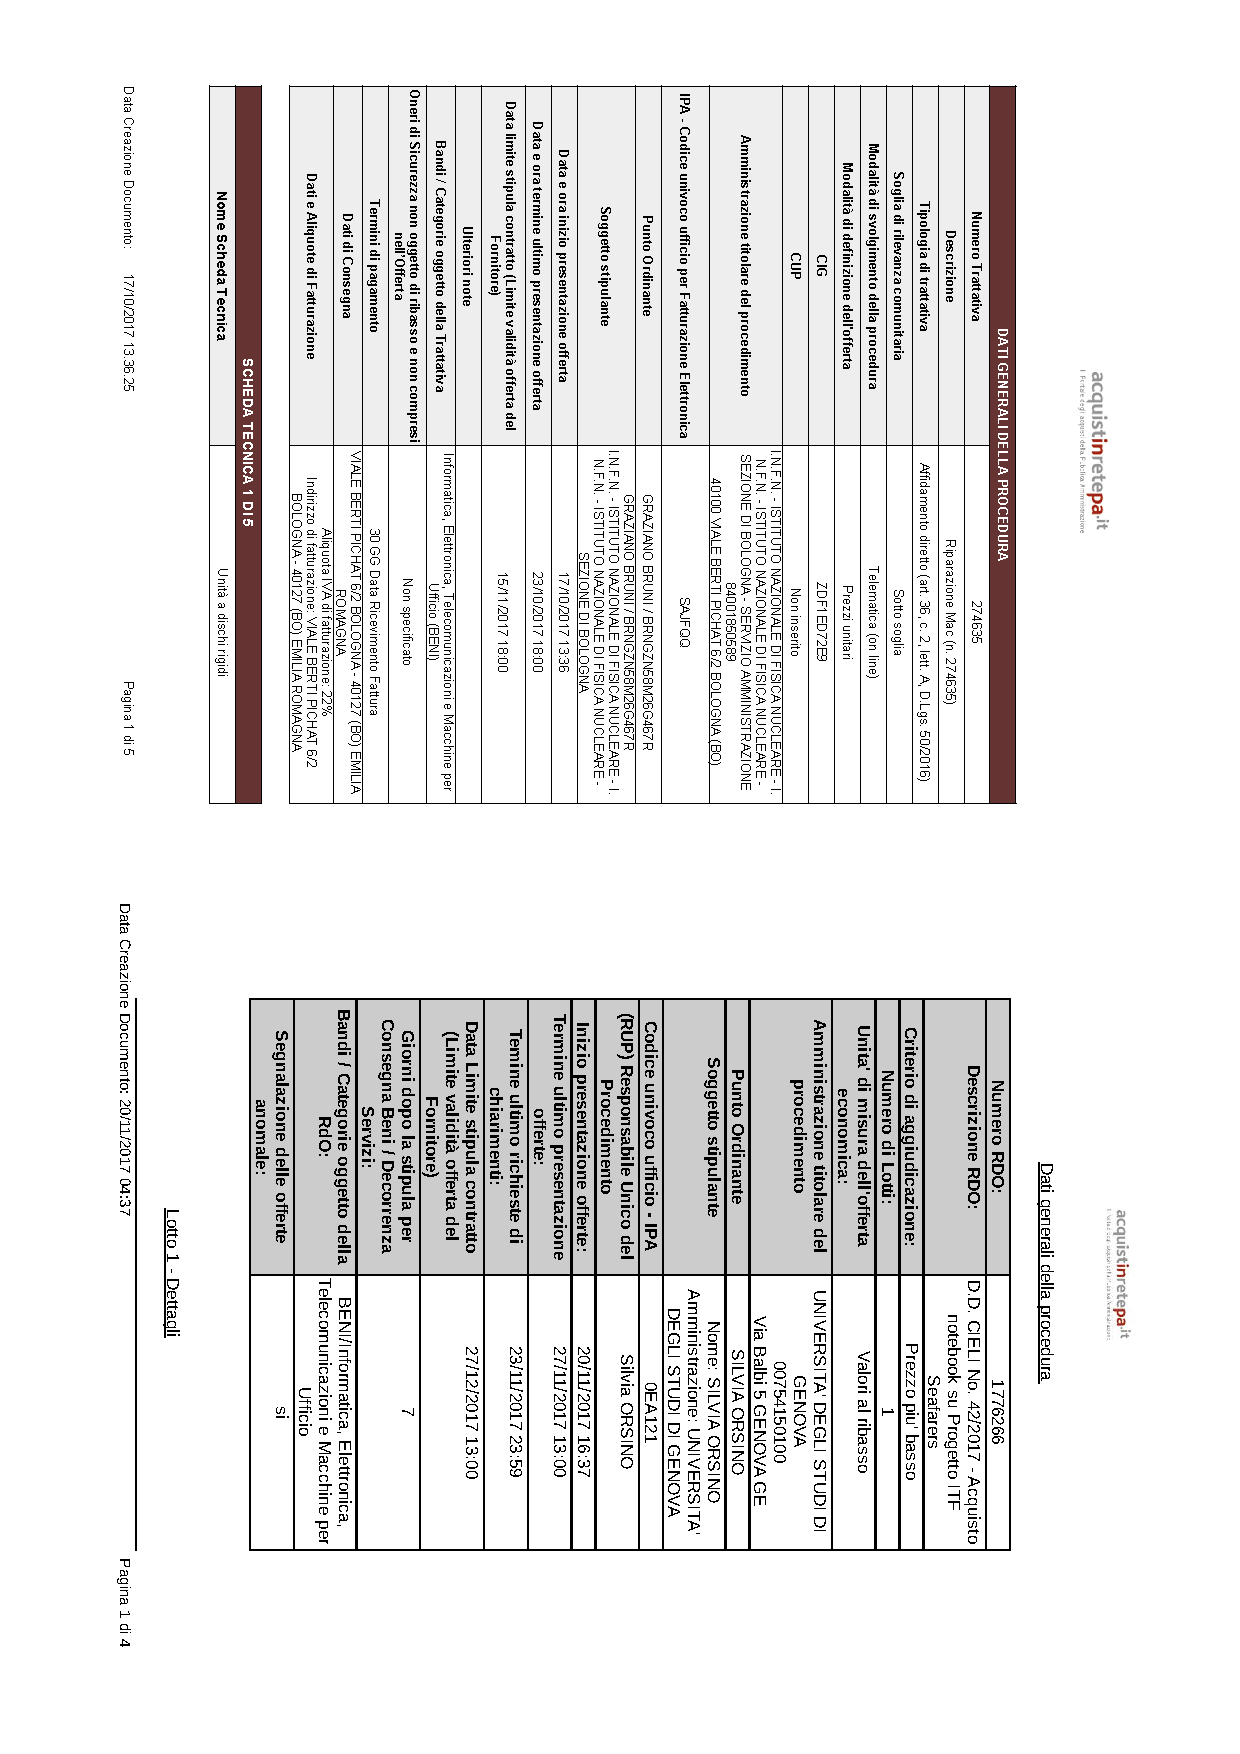
\includepdf[]{./pdf/moduli2.pdf}
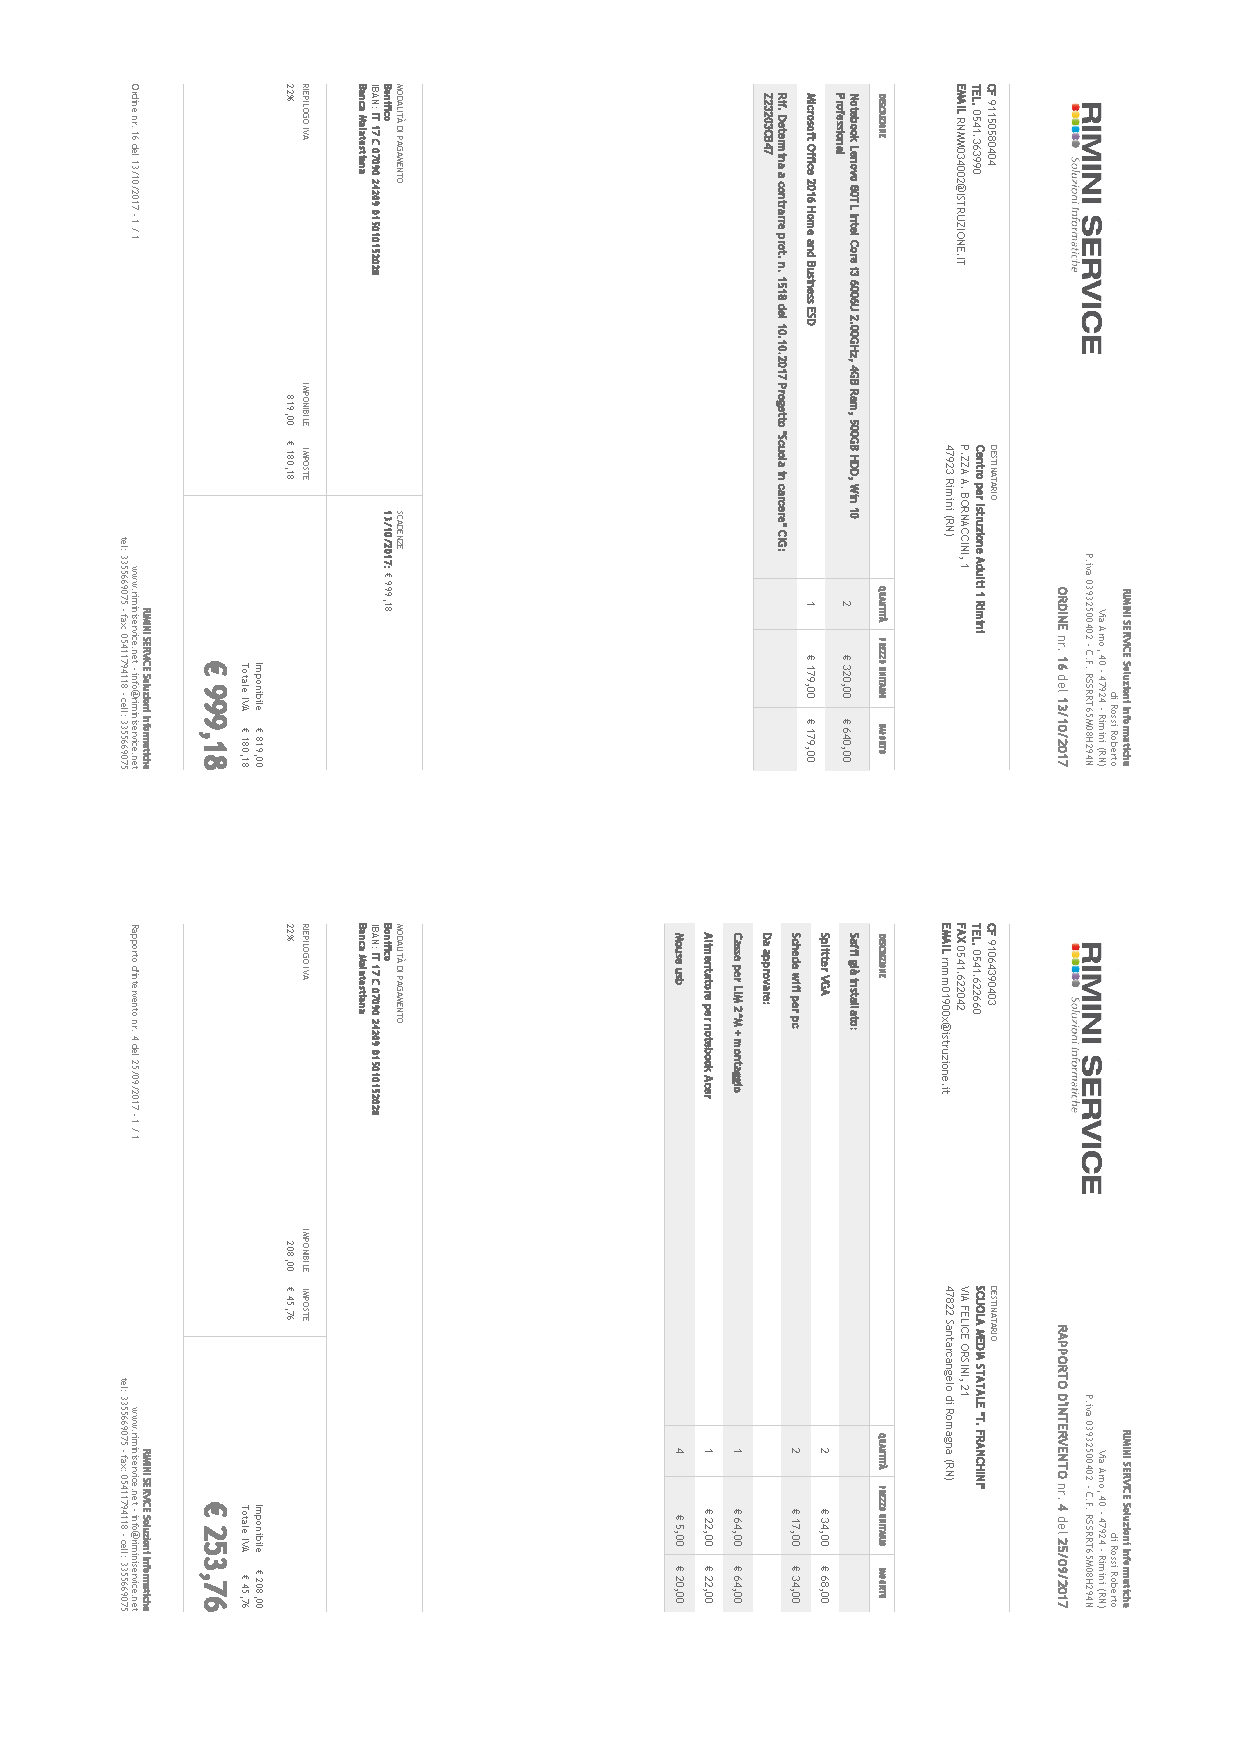
\includepdf[]{./pdf/moduli.pdf}

%-------------------------------------------------------------------------
\subsubsection{Analisi delle Azioni e dei Processi Interni}

Partendo dalle interviste e utlizzando i documenti forniti, abbiamo voluto organizzare le informazioni in uno schema dei processi interni, per poter avere una miglior comprensione del flusso di operazioni interne all'azienda. Abbiamo costruito uno schema piuttosto informale, in cui sono presenti ridondanze che verranno analizzate in seguito. E' possibile osservare il flusso di operazioni partendo da un contatto tra cliente e azienda, che può avvenire in 3 modi: un privato contatta l'azienda, una pubblica amministrazione contatta l'azienda attraverso una trattativa diretta, oppure l'azienda si mette in contatto con una pubblica amministrazione attraverso una gara pubblica.\newline
Segue lo schema:\newline\newline\newline\newline\newline

\noindent\makebox[\textwidth]{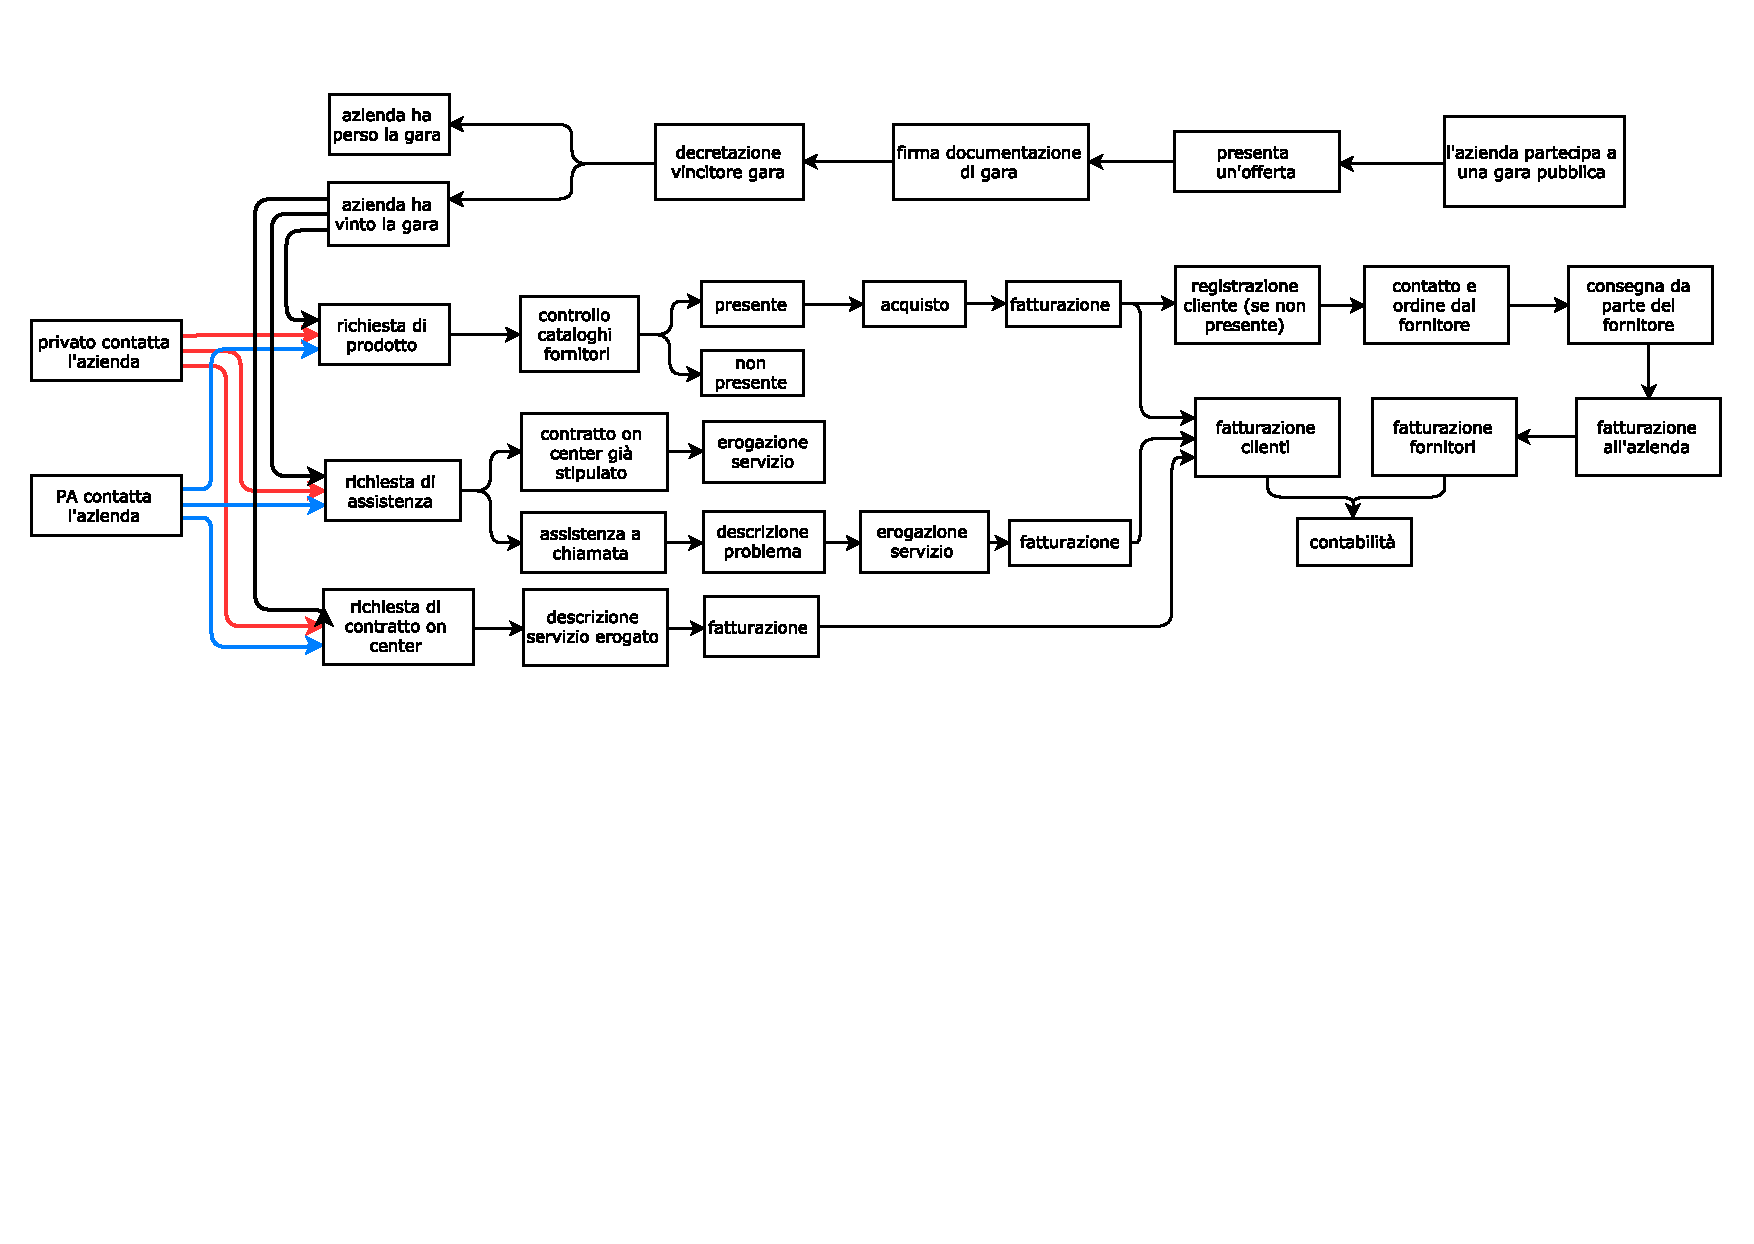
\includegraphics[width=\paperwidth-1cm, trim={0 8cm 0 0}, clip]{./immagini/processi_interni.pdf}}


% \newpage
%
% \begin{landscape} %inizia un foglio landscape
%
%
% %include un file pdf che contiene lo schema ruotato e dimensionato correttamente
% 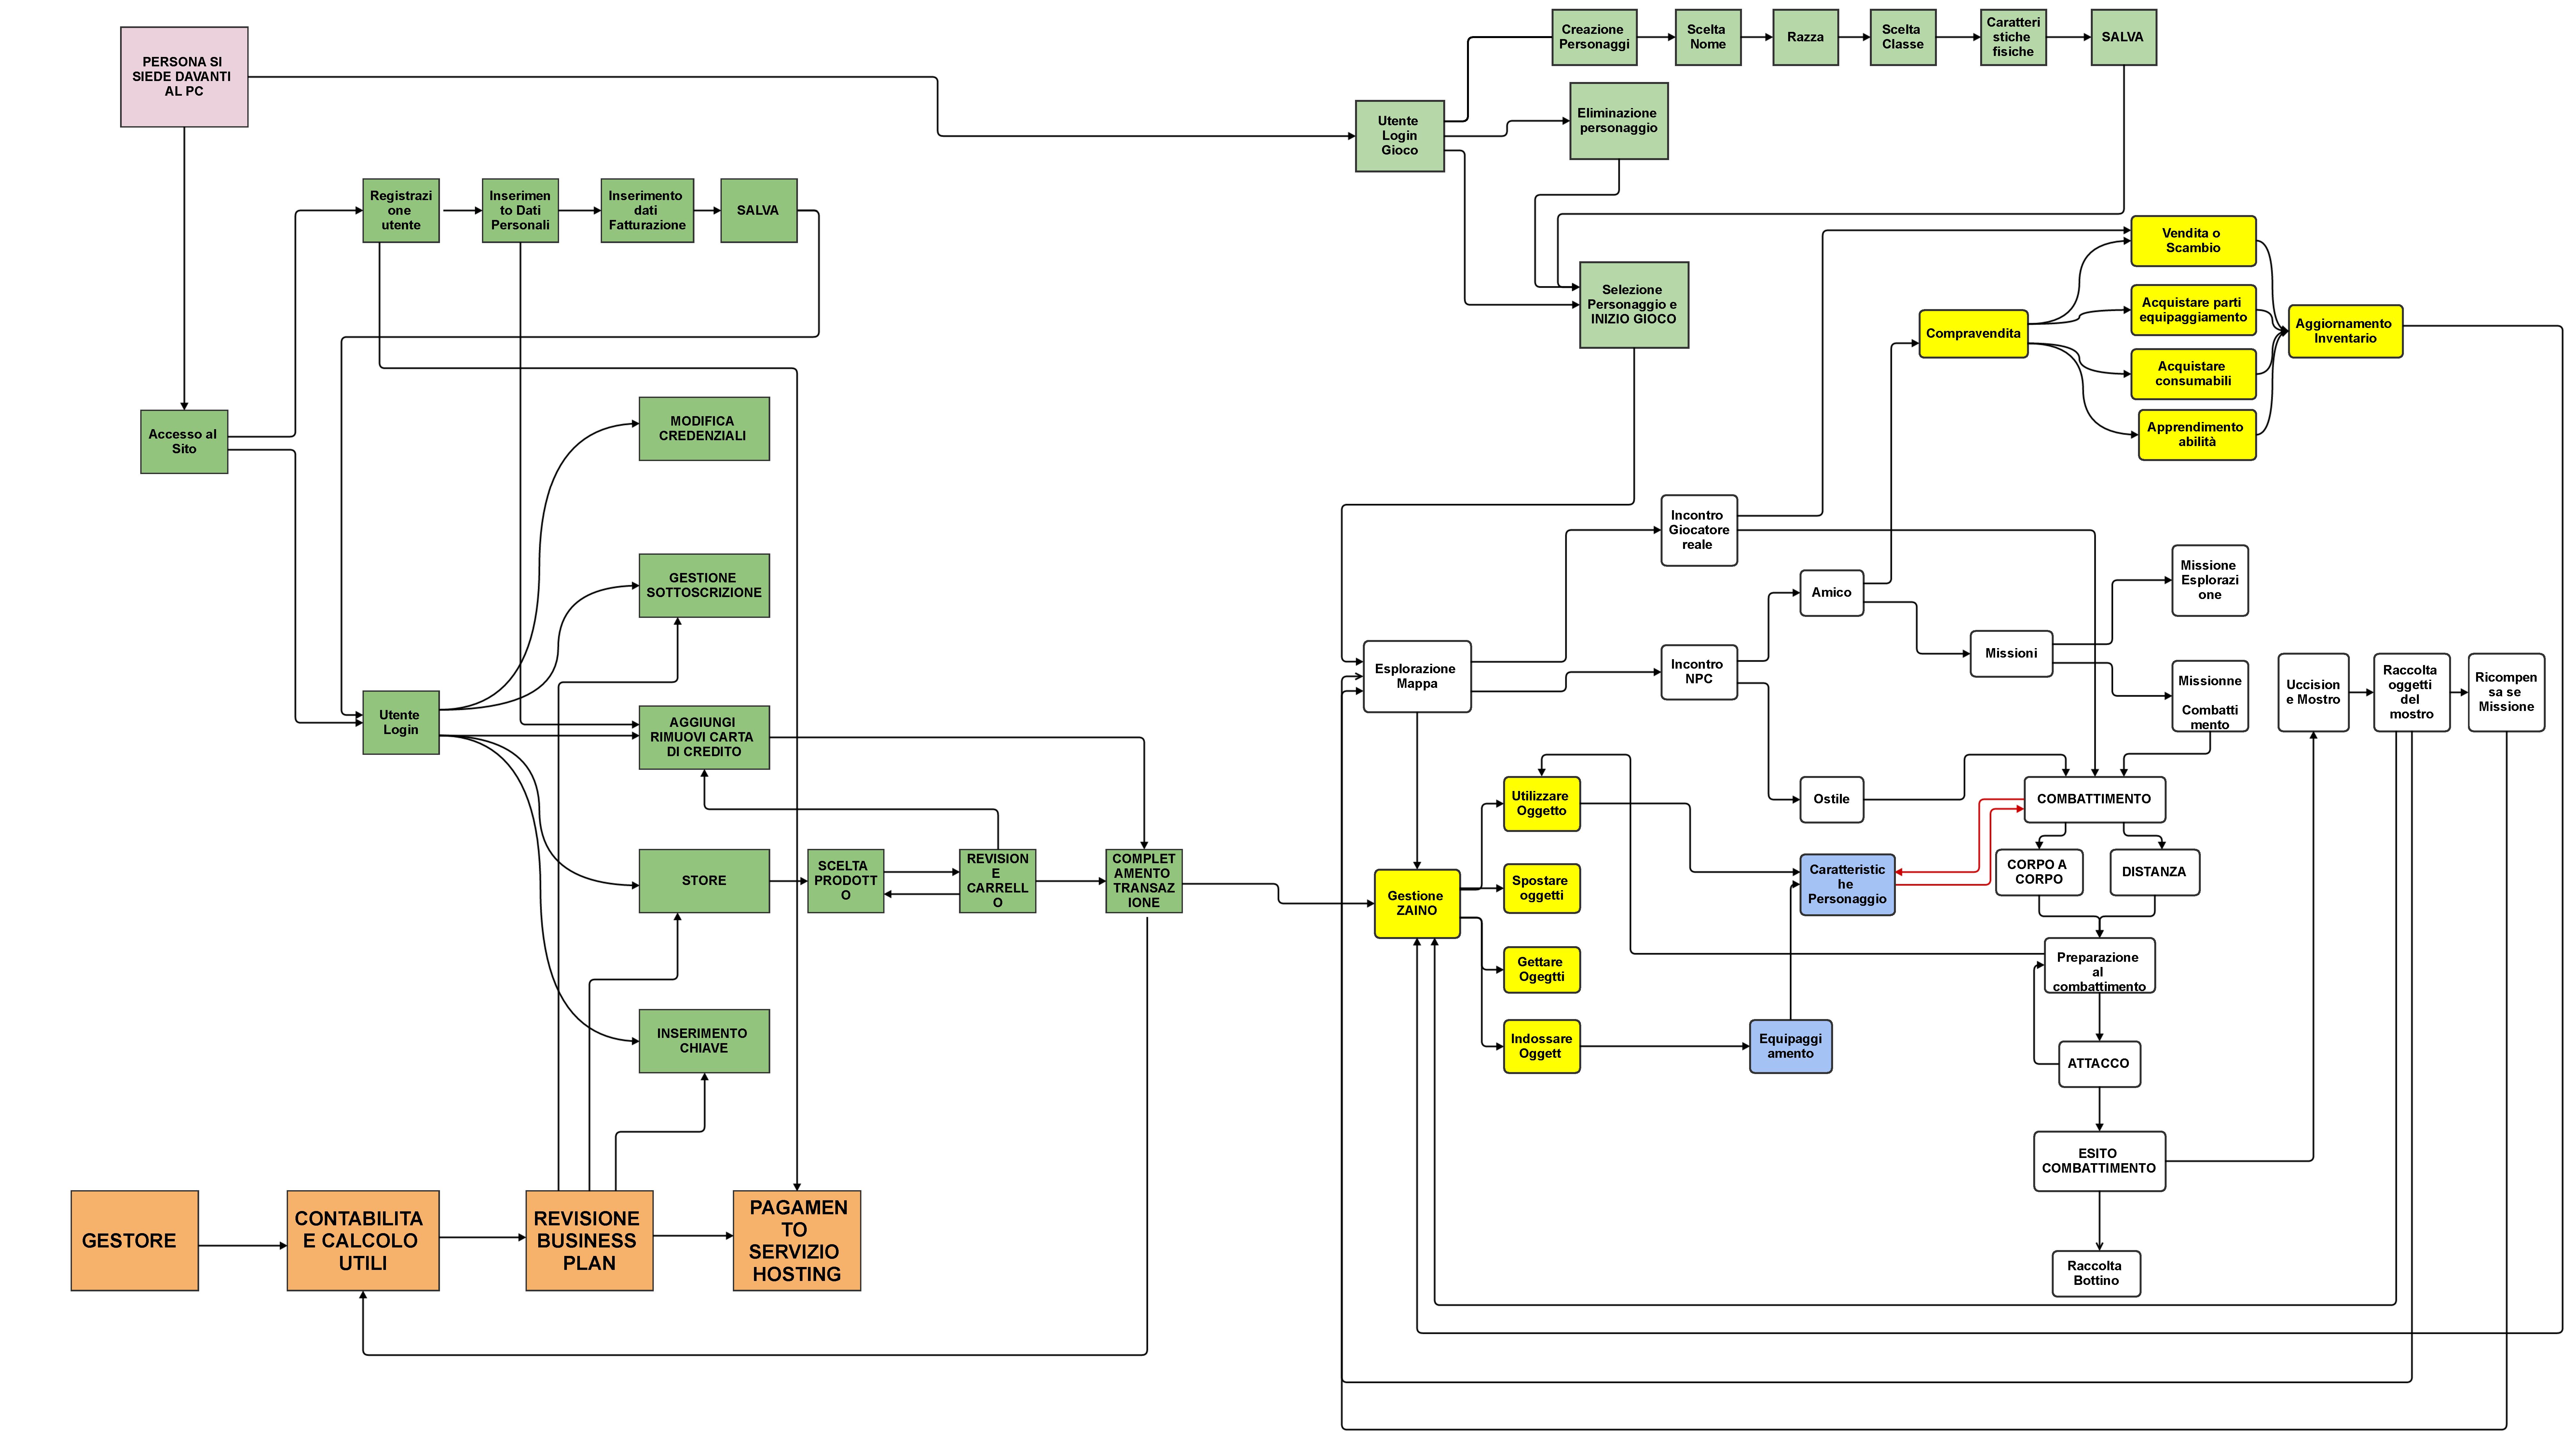
\includepdf[width=270mm, height=210mm, angle=90, keepaspectratio]{./pdf/sprocint.pdf}
% 
% \end{landscape}

		%inserire allegati
		%-----------------------------------------------------------------------
		\subsection{Requisiti Espressi nel Linguaggio Naturale}

		
Dopo aver analizzato le interviste effettuate e i documenti allegati, è stato possibile stabilire gli obiettivi che effettivamente vorremmo che la nostra base di dati raggiunga.
Il nostro scopo è realizzare un database che organizzi i dati di una azienda che vende prodotti e servizi sia a \hl{privati}, che a \hl{pubbliche amministrazioni} partecipando a gare pubbliche.

% Pensiamo che la nostra base dati duri almeno X anni, perchè bla bla ..

\noindent
\newline
Quindi si dovranno gestire i dati relativi a gare pubbliche del mercato elettronico, ai clienti, ai fornitori esterni, ai prodotti, ai servizi offerti, alle stipule di contratto.

\noindent
\newline
Siamo interessati a tenere traccia di tutte le \hl{gare pubbliche} a cui si partecipa (sia vinte, sia perse), per verificare la "forza economica" dell'azienda sul mercato e per conoscere i prezzi di vendita dei concorrenti.
Inoltre vogliamo tenere traccia dei prodotti e dei servizi più venduti dall'azienda stessa, per scopi statistici.

\noindent
\newline
Per quanto riguarda le gare pubbliche, si vogliono inserire dati relativamente ai prodotti/servizi richiesti, al tetto massimo di spesa, all'\hl{aggiudicatario della gara}, e al prezzo proposto dall'aggiudicatario della gara.

\noindent
\newline
Relativamente ai \hl{clienti}, si registreranno dati relativi alla ragione sociale e recapiti, e nel caso il cliente sia una pubblica amministrazione verrà inserito anche il codice PA e l'indirizzo PEC associati ad essa.

\noindent
\newline
Riguardo ai \hl{fornitori} dell'azienda, si vogliono inserire dati relativi alla ragione sociale, i recapiti, il \hl{catalogo prodotti} e la tabella per il calcolo delle \hl{spese di spedizione}.
Di ogni \hl{prodotto} vogliamo conoscere il codice prodotto, le caratteristiche generali (per poter partecipare a gare in cui non sono richiesti prodotti specifici), il prezzo (relativo a un dato fornitore), il peso e le dimensioni per il calcolo dei costi di spedizione.

\noindent
\newline
Relativamente ai \hl{servizi}, si vuole tenere traccia della lista dei servizi offerti, e la stima del costo di una prestazione (ad esempio: formattazione di 1 PC: 50 \euro, sostituzione di 1 hard disk: 35 \euro)

\noindent
\newline
Per ognuno dei \hl{contratti} stipulati, si vuole conoscere la controparte con cui questi vengono stipulati, la data, la tipologia (vendita prodotto, assistenza), l'importo, e, nel caso di contratti di assistenza on center, la data di inizio e scadenza del contratto.

\newpage


		%------------------------------------------------
		\subsection{Glossario dei Termini}

		%Se non si vuole creare la tablella in latex è possibile farla con word, copincollarla
%nella sezione File/paste table data del sito http://www.tablesgenerator.com
%che genererà la tabella in latex
%non scordare di mettere le chiusure di table e di adjustbox

% Comando per fare le celle su più righe, separa ogni riga con '\\'
\newcommand{\specialcell}[2]{
  \begin{tabular}[t]{@{}l@{}}#1\end{tabular}} % [c] centra in verticale

\begin{table}[h!]
  \centering
  \begin{adjustbox}{width=\textwidth}
    \begin{tabular}{@{}llll@{}}
      \toprule
      \textbf{TERMINE} & \textbf{DESCRIZIONE} & \textbf{SINONIMI} & \textbf{COLLEGAMENTO} \\ \midrule

      \multicolumn{1}{|l|}{\specialcell{Pubblica amministrazione \\ (PA)}}
      & \multicolumn{1}{l|}{\specialcell{Entità giuridica che persegue fini \\ di interesse pubblico.}}
      & \multicolumn{1}{l|}{}
      & \multicolumn{1}{l|}{Cliente, MEPA} \\ \midrule

      \multicolumn{1}{|l|}{Privato (ente)}
      & \multicolumn{1}{l|}{\specialcell{Entità giuridica che persegue fini \\ di interesse privato di tipo economico e sociale.}}
      & \multicolumn{1}{l|}{}
      & \multicolumn{1}{l|}{Cliente} \\ \midrule

      \multicolumn{1}{|l|}{Cliente}
      & \multicolumn{1}{l|}{\specialcell{Entità fisica o giuridica che abbia mai \\ acquistato un prodotto o servizio dall'azienda.}}
      & \multicolumn{1}{l|}{Acquirente}
      & \multicolumn{1}{l|}{Privato, PA} \\ \midrule

      \multicolumn{1}{|l|}{\specialcell{Mercato delle \\ Pubbliche \\ Amministrazioni \\ (MEPA)}}
      & \multicolumn{1}{l|}{\specialcell{Mercato digitale in cui le Amministrazioni \\ abilitate possono acquistare, per valori \\ inferiori alla soglia comunitaria, i beni \\ e servizi offerti da fornitori abilitati.}}
      & \multicolumn{1}{l|}{}
      & \multicolumn{1}{l|}{\specialcell{PA, RDO, \\ Fornitore abilitato}} \\ \midrule

      \multicolumn{1}{|l|}{\specialcell{Fornitore abilitato \\ al MEPA}}
      & \multicolumn{1}{l|}{\specialcell{Azienda abilitata ad offrire i suoi prodotti \\ e servizi sul MEPA.}}
      & \multicolumn{1}{l|}{}
      & \multicolumn{1}{l|}{MEPA} \\ \midrule

      \multicolumn{1}{|l|}{\specialcell{Richiesta di offerta \\ (RDO)}}
      & \multicolumn{1}{l|}{\specialcell{Gara pubblica promossa da una PA in cui \\ essa richiede determinati prodotti e/o servizi.}}
      & \multicolumn{1}{l|}{Gara pubblica}
      & \multicolumn{1}{l|}{MEPA} \\ \midrule

      \multicolumn{1}{|l|}{\specialcell{Aggiudicatario di \\ una gara}}
      & \multicolumn{1}{l|}{\specialcell{Azienda abilitata al MEPA che ha ottenuto \\ la fornitura relativa a una richiesta di offerta.}}
      & \multicolumn{1}{l|}{Vincitore}
      & \multicolumn{1}{l|}{Richiesta di offerta} \\ \midrule

      \multicolumn{1}{|l|}{Trattativa diretta}
      & \multicolumn{1}{l|}{\specialcell{Trattativa che una PA invia direttamente \\ ad un'azienda abilitata al MEPA}}
      & \multicolumn{1}{l|}{}
      & \multicolumn{1}{l|}{PA, Fornitore abilitato} \\ \midrule

      \multicolumn{1}{|l|}{Trattativa stipulata}
      & \multicolumn{1}{l|}{\specialcell{L'azienda accetta le condizioni \\ di una trattativa diretta.}}
      & \multicolumn{1}{l|}{}
      & \multicolumn{1}{l|}{Trattativa diretta} \\ \midrule

      \multicolumn{1}{|l|}{Fornitore (esterno)}
      & \multicolumn{1}{l|}{\specialcell{Azienda esterna che collabora con l'azienda \\ in questione per la vendita di prodotti alle PA.}}
      & \multicolumn{1}{l|}{\specialcell{Dropshipper, \\ Venditore}}
      & \multicolumn{1}{l|}{\specialcell{Dropshipping, RDO, \\ Trattativa diretta}} \\ \midrule

      \multicolumn{1}{|l|}{Prodotto}
      & \multicolumn{1}{l|}{\specialcell{Un qualsiasi prodotto reso disponibile \\ da un fornitore esterno.}}
      & \multicolumn{1}{l|}{}
      & \multicolumn{1}{l|}{\specialcell{Fornitore (esterno), \\ MEPA, Cliente}} \\ \midrule

      \multicolumn{1}{|l|}{Dropshipping}
      & \multicolumn{1}{l|}{\specialcell{Vendita di un prodotto ad un cliente senza \\ possederlo materialmente nel proprio magazzino.}}
      & \multicolumn{1}{l|}{}
      & \multicolumn{1}{l|}{\specialcell{Fornitore (esterno), \\ Prodotto}} \\ \midrule

      \multicolumn{1}{|l|}{Catalogo}
      & \multicolumn{1}{l|}{\specialcell{Catalogo di prodotti offerti \\ da un particolare fornitore esterno.}}
      & \multicolumn{1}{l|}{}
      & \multicolumn{1}{l|}{Fornitore (esterno)} \\ \midrule

      \multicolumn{1}{|l|}{Servizio}
      & \multicolumn{1}{l|}{\specialcell{Servizio offerto dall'azienda in questione.}}
      & \multicolumn{1}{l|}{}
      & \multicolumn{1}{l|}{Cliente} \\ \midrule

      \multicolumn{1}{|l|}{Contratto}
      & \multicolumn{1}{l|}{\specialcell{Atto che stipula un accordo di vendita \\ o acquisto fra l'azienda e una controparte.}}
      & \multicolumn{1}{l|}{}
      & \multicolumn{1}{l|}{\specialcell{Cliente, Prodotto, \\ Assistenza}} \\ \midrule

      \multicolumn{1}{|l|}{Assistenza "on center"}
      & \multicolumn{1}{l|}{\specialcell{Servizio di assistenza erogata a domicilio \\ dall'azienda in questione a un suo cliente.}}
      & \multicolumn{1}{l|}{}
      & \multicolumn{1}{l|}{Cliente, Contratto} \\ \midrule

      \multicolumn{1}{|l|}{Assistenza a chiamata}
      & \multicolumn{1}{l|}{\specialcell{Servizio di assistenza senza vincoli \\ erogato con interventi a richiesta del cliente.}}
      & \multicolumn{1}{l|}{}
      & \multicolumn{1}{l|}{Cliente} \\ \midrule

      % \multicolumn{1}{|l|}{Ordine}
      % & \multicolumn{1}{l|}{\specialcell{Ordine di prodotti effettuato a un fornitore.}}
      % & \multicolumn{1}{l|}{}
      % & \multicolumn{1}{l|}{Prodotto} \\ \midrule

      \multicolumn{1}{|l|}{Costo di spedizione}
      & \multicolumn{1}{l|}{\specialcell{Costo associato a un ordine a un fornitore, che \\ dipende da volume e peso dei prodotti da consegnare.}}
      & \multicolumn{1}{l|}{}
      & \multicolumn{1}{l|}{Prodotto, Fornitore} \\ \midrule

      % \multicolumn{1}{|l|}{Margine di guadagno}
      % & \multicolumn{1}{l|}{\specialcell{Persona fisica che gestisce e gestisce \\ e controlla il personaggio.}}
      % & \multicolumn{1}{l|}{Giocatore}
      % & \multicolumn{1}{l|}{Personaggio} \\ \midrule


    \end{tabular}
  \end{adjustbox}
\end{table}

		\newpage
		%------------------------------------------------
		\subsection{Eliminazione delle Ambiguit\'{a} Presenti}

		L'unica fonte di ambiguità è data dalla definizione di fornitore, in quanto i fornitori abilitati al MEPA sono proprio i venditori che possono partecipare alle gare pubbliche, come la nostra azienda. I fornitori esterni sono invece le aziende a cui noi ci rivolgiamo per acquistare e poi rivendere i prodotti.

		%------------------------------------------------
		\subsection{Strutturazione dei Requisiti}

		
\subsubsection{Frasi di Carattere Generale}
L'azienda necessita di interfacciarsi con diverse entità, fungendo da intermediaria indipendente, rispondendo alle richieste di gare pubbliche attraverso la disponibilità di fornitori privati. In tutto ciò la nostra base di dati può risultare fondamentale per l'ottimizzazione dei processi e in più per fornire importanti analisi su ciò che offre il mercato e quali migliorie possono essere apportate, così da ottimizzare non solo i processi, ma il business stesso.\newline
Si gestiranno perciò i dati riguardanti le gare pubbliche, i clienti, i fornitori, i prodotti, i servizi e tutte le tipologie di contratti stipulati tra l'azienda e i clienti.

\subsubsection{Frasi relative alle Gare Pubbliche}
Le gare pubbliche vengono pubblicate sul sito acquistinretepa.it, cioè il Portale degli acquisti della Pubblica Amministrazione di proprietà del Ministero dell'Economia e delle Finanze e del Consip.\newline
La sezione di interesse per l'azienda è quella del Mercato Elettronico delle Pubbliche Amministrazioni, chiamato MEPA. Qui le imprese possono vedere le gare pubbliche e parteciparvi.\newline
Un'azienda abilitata alla vendita sul MEPA, necessita di credenziali di accesso al sito suddetto, in questo modo può partecipare ad un numero illimitato di gare.\newline
L'iscrizione a una gara consiste nel effettuare un'offerta, e dalla richiesta di offerta possono essere ottenute tutte le informazioni sulla richiesta e il richiedente, cioè la pubblica amministrazione che ha eseguito la richiesta, con tanto di codice identificativo PA.\newline
Quindi è importante registrare tutte le informazioni. L'idea è quella di registrare non solamente le gare aggiudicate, ma anche quelle perse, in modo da poter effettuare delle analisi successive. La quantità di gare presenti permette di effettuare questo tipo di operazione manualmente. Potrebbe essere previsto un web scraper in fase avanzata che gestisca in automatico questa procedura.\newline
La registrazione è determinata da due fasi, quella iniziale in cui si accingono i dati generali sulla gara e sul cliente, e poi una fase finale, dopo la chiusura della gara, per raccogliere dati sugli aggiudicatari e l'offerta effettuata, sempre a scopo di analisi.

\subsubsection{Frasi relative ai Clienti}
Per quel che riguarda i clienti, si hanno sia enti privati che pubbliche amministrazioni. Per gli enti privati sono necessari i dati relativi alla ragione sociale, l'indirizzo, dati di fatturazione. Per le pubbliche amministrazioni, oltre a questi dati, servono informazioni riguardo al codice PA e all'indirizzo di posta PEC, tutte informazioni estraibili dalle richieste di offerta sul MEPA. \newline
Sia ai privati e sia alle pubbliche amministrazioni saranno poi legati i contratti e le fatture, nelle apposite tabelle.

\subsubsection{Frasi relative alle Assistenze}
Le assistenze si dividono in assistenze di due tipi:
\begin{itemize}
\item	assistenze on center;
\item	assistenze a chiamata;
\end{itemize}
Le assistenze on center sono erogate a domicilio, in seguito alla stipulazione di un contratto di durata prestabilita, solitamente dai quattro mesi a un anno, per cui il cliente paga una quota fissa in modo da ricevere assistenza sul luogo in base alle sue esigenze.\newline
I dati importanti al riguardo sono il costo del contratto, la data di inizio e la data di scadenza, e il tipo di assistenza.\newline
Le assistenze a chiamata non sono vincolate da uno contratto, il cliente può chiedere interventi su richiesta e paga a prestazione compiuta.
In questo caso si registrano la data in cui si è fatta assistenza, il tipo di servizio erogato, e il cliente che ha ricevuto assistenza.


\subsubsection{Frasi relative ai Prodotti}
I prodotti sono quelli messi a disposizione dai fornitori, i quali forniscono i propri cataloghi che comprendono una lista di codici prodotto con il relativo prezzo di vendita. I dati quindi da registrare sono soprattutto il codice prodotto, in quanto spesso i clienti chiedono un prodotto in base al codice specifico, e le caratteristiche tecniche del prodotto.\newline
In seguito alla vendita di un prodotto viene emessa una fattura al cliente con indicati i prodotti venduti, i costi, e i dati relativi a venditore e acquirente.

\subsubsection{Frasi relative ai Servizi}
I servizi sono entità particolari che necessitano di una standardizzazione nella loro trattazione in quanto il costo è molto variabile e non è determinato per forza in base al tempo speso per effettuare tale servizio. I servizi devono essere registrati con il loro costo, e deve essere strutturata una descrizione generica da poter riportare. Il servizio di per sè implica anche uno spostamento di cui tener conto, che potrebbe essere comparato a quelli che sono i costi di spedizione in caso di acquisto di un prodotto.\newline
Dopo l'erogazione di un servizio viene emessa una fattura al cliente che deve riportare la prestazione eseguita, il costo, e i dati relativi al fornitore e al ricevente del servizio.

\subsubsection{Frasi relative ai Fornitori}
I fornitori sono coloro da cui vengono acquistati i prodotti da vendere ai clienti. I dati necessari al riguardo sono simili a quelli dei clienti, quindi bisogna registrare ragione sociale, indirizzo, dati di fatturazione per i pagamenti. Ad essi è importante legare i catalogi forniti, che vengono consultati per verificare la disponibilità dei prodotti, e vengono aggiornati mensilmente.

\subsubsection{Frasi relative alle Fatture}
Si vogliono conoscere le informazioni relative a una fattura, sia in entrata che in uscita. Sono quindi necessari il codice del contratto a cui si riferisce, la data di emissione, la data entro cui è necessario pagare.

% \subsubsection{Frasi relative agli Ordini}
% Gli ordini rappresentano i prodotti acquistati dai fornitori. Spesso gli ordini effettuati non sono spediti all'azienda che deve poi spedirli ai clienti, ma vengono direttamente spediti al cliente, seguendo il modello di dropshipping. In ogni caso bisogna tener traccia anche dei costidi spedizone}, oltre che al prodotto interessato dall'ordine e le sue caratteristiche, il costo dell'ordine, il fornitore del prodotto, il cliente che ha acquistato il prodotto per cui è stato effettuato l'ordine. Tutto ciò implica la connessione di diverse entità interessate che insieme vanno a formare l'ordine. Qui come nelle trattative bisogna considerare la fattura, in particolare la fattura emessa ai clienti da parte della azienda, e in questo caso la fattura emessa dal fornitore all'azienda per l'acquisto.


		%------------------------------------------------
		\subsection{Specifica delle Operazioni}

		
% Calcoli fatti considerando una media di 3500 utenti connessi al server. Ad esclusione delle operazioni fatte ogni 3 anni che vengono svolte dagli sviluppatori al rilascio delle nuove espansioni. La 34,35,36 vengono fatte con le patch mensili per bilanciare il gioco.

Assumptions: Numero fornitori: 10

\begin{enumerate}

  \item Inserimento nuovo cliente (in media 10 volte al mese)
  \item Inserimento nuova gara pubblica (in media una volta al giorno)
  \item Inserimento nuova trattativa diretta (in media una volta a settimana)
  \item Inserimento nuovo prodotto (due volte al mese)
  \item Inserimento nuovo servizio (due volte all'anno)
  \item Inserimento nuovo contratto di assistenza on center (una volta al mese)
  \item Inserimento nuova fattura (in media tre volte al giorno)
  \item Inserimento nuovo fornitore (due volte all'anno)
  \item Inserimento di un nuovo catalogo (due volte all'anno)
  \item Inserimento nuova tabella di costi di spedizione (due volte all'anno)
  \item Aggiornamento di una gara pubblica in seguito alla sua chiusura (in media una volta al giorno)
  \item Aggiornamento di una trattativa diretta in seguito alla sua stipula (in media una volta a settimana)
  \item Aggiornamento di un catalogo (dieci volte al mese)
  \item Aggiornamento di una tabella di costi di spedizione (in media due volte all'anno)
  \item Modifica dati cliente (in media 20 volte all'anno)
  \item Modifica dati di un servizio (in media due volte all'anno)
  \item Modifica dati di un fornitore (in media tre volte all'anno)
  \item Cancellazione di un prodotto (quattro volte all'anno)
  \item Cancellazione di un servizio (in media una volta all'anno)
  \item Cancellazione di un fornitore (una volta all'anno)
  \item Cancellazione di un catalogo (una volta all'anno)
  \item Consultazione dati dei clienti (in media 10 volte al giorno)
  \item Consultazione dati dei fornitori (in media due volte al giorno)
  \item Consultazione contratti di assistenza on center (in media due volte a settimana)
  \item Consultazione contratti di assistenza on center in un determinato periodo (due volte al mese)
  \item Consultazione dati di una gara pubblica (in media cinque volte al giorno)
  \item Consultazione dati di una trattativa diretta (in media due volte al giorno)
  \item Consultazione caratteristiche di un prodotto (cinque volte al giorno)
  \item Consultazione prezzo di un prodotto (dieci volte al giorno)
  \item Consultazione di una fattura (una volta al giorno)
  \item Statistica delle gare pubbliche vinte e perse in un determinato periodo (una volta al mese)
  \item Statistica delle trattative dirette stipulate (una volta al mese)
  \item Statistica dei prodotti più venduti (una volta al mese)
  \item Statistica dei servizi più erogati (una volta al mese)
  \item Verifica del pagamento delle fatture da parte dei clienti (due volte a settimana)
  \item Verifica di scadenza imminente del pagamento delle fatture da parte dei clienti (tre volte al mese)
  \item Verifica del pagamento delle fatture da parte dell'azienda (due volte a settimana)
  \item Verifica di scadenza imminente del pagamento delle fatture da parte dell'azienda (tre volte al mese)
  \item Calcolo del guadagno netto ad una certa data (una volta al mese)
  \item Calcolo del volume di vendite in un determinato periodo (una volta al mese)
  \item Calcolo dei costi di spedizione di un'acquisto (tre volte al giorno)
  \item Selezione della migliore combinazione di prodotti (tre volte al giorno)
  \item Selezione che tiene conto dei margini di guadagno e dei volumi (si può fare?) Considerare margini (standard: 10%, ma si può abbassare) ()

\end{enumerate}


		\newpage

%------------------------------------------------
	\section{Progettazione Concettuale}


		\subsection{Strategia di Progetto }
			Analizzando nel loro insieme l'inservista e lo schema delle azioni e dei processi interni, abbiamo potuto estrapolare il flusso aziendale, così da capire esattamente le problematiche e le aree in cui intervenire, implementando la nostra base di dati.\newline \newline
			In questo modo abbiamo potuto concepire l'approccio migliore da seguire, sfruttando un approccio misto tra il TOP-DOWN, e il BOTTOM-UP, sbilanciato però verso il primo dei due. Le  fasi sono state:
			\begin{enumerate}
			\item Analisi intervista e processi interni per l'analisi generale del flusso aziendale
			\item Creazione schema scheletro composto dalle entità principali
			\item Approccio TOP-DOWN: sviluppo dettagliato delle principali entità presenti
			\item Approccio BOTTOM-UP: generalizzazione e accorpamento delle varie entità nello schema completo
			\end{enumerate}

		%------------------------------------------------
		\subsection{Individuazione Entità e Relazioni Principali}

		Come precedentemente specificato sono state estrapolate le entità principali intorno alle quali sviluppare la progettazione. Ciò è stato possibile grazie ad un'approfondita analisi del flusso aziendale, derivato direttamente dall'analisi delle azioni e dei processi interni.\newline
Il risultato è dato dalle cinque seguenti entità fondamentali: \newline

\noindent\makebox[\textwidth]{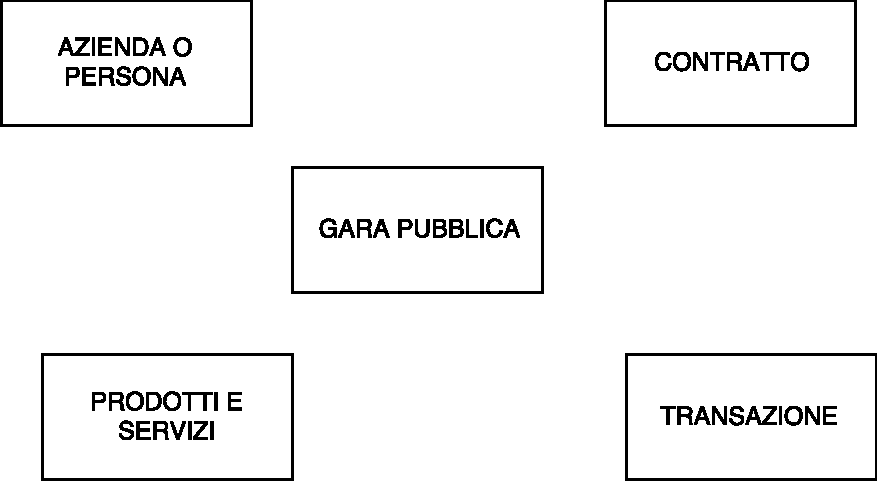
\includegraphics[width=\textwidth-5cm]{./immagini/entita_fondamentali.pdf}}
\newline
\newline
RICHIESTA SUL MEPA: il blocco rappresenta gli strumenti che le pubbliche amministrazioni utilizzano per  l'interfacciamento con la nostra azienda. In questo caso si parla di gare pubbliche oppure richieste di trattativa dirette. \newline
PA, AZIENDA O PERSONA: è il macrogruppo comprensivo delle persone giuridiche che hanno rapporti commerciali con la nostra azienda, tra questi ci sono i fornitori e i clienti, sia privati e pubbliche amministrazioni.\newline
PRODOTTO O SERVIZIO: comprende tutti i prodotti vendibili o acquistabili dall'azienda disponibili dai fornitori e i servizi disponibili.\newline
FATTURA: è l'entità fondamentale che interviene in tutte le operazioni sia per l'acquisto che per la vendita di prodotti e/o servizi.

\newpage


		%------------------------------------------------
		\begin{landscape}

		\subsection{Scheletro dello Schema ER}
			Possiamo unire le Componenti principali nel seguente schema scheletro:

			\begin{figure}[H]
			\centering
			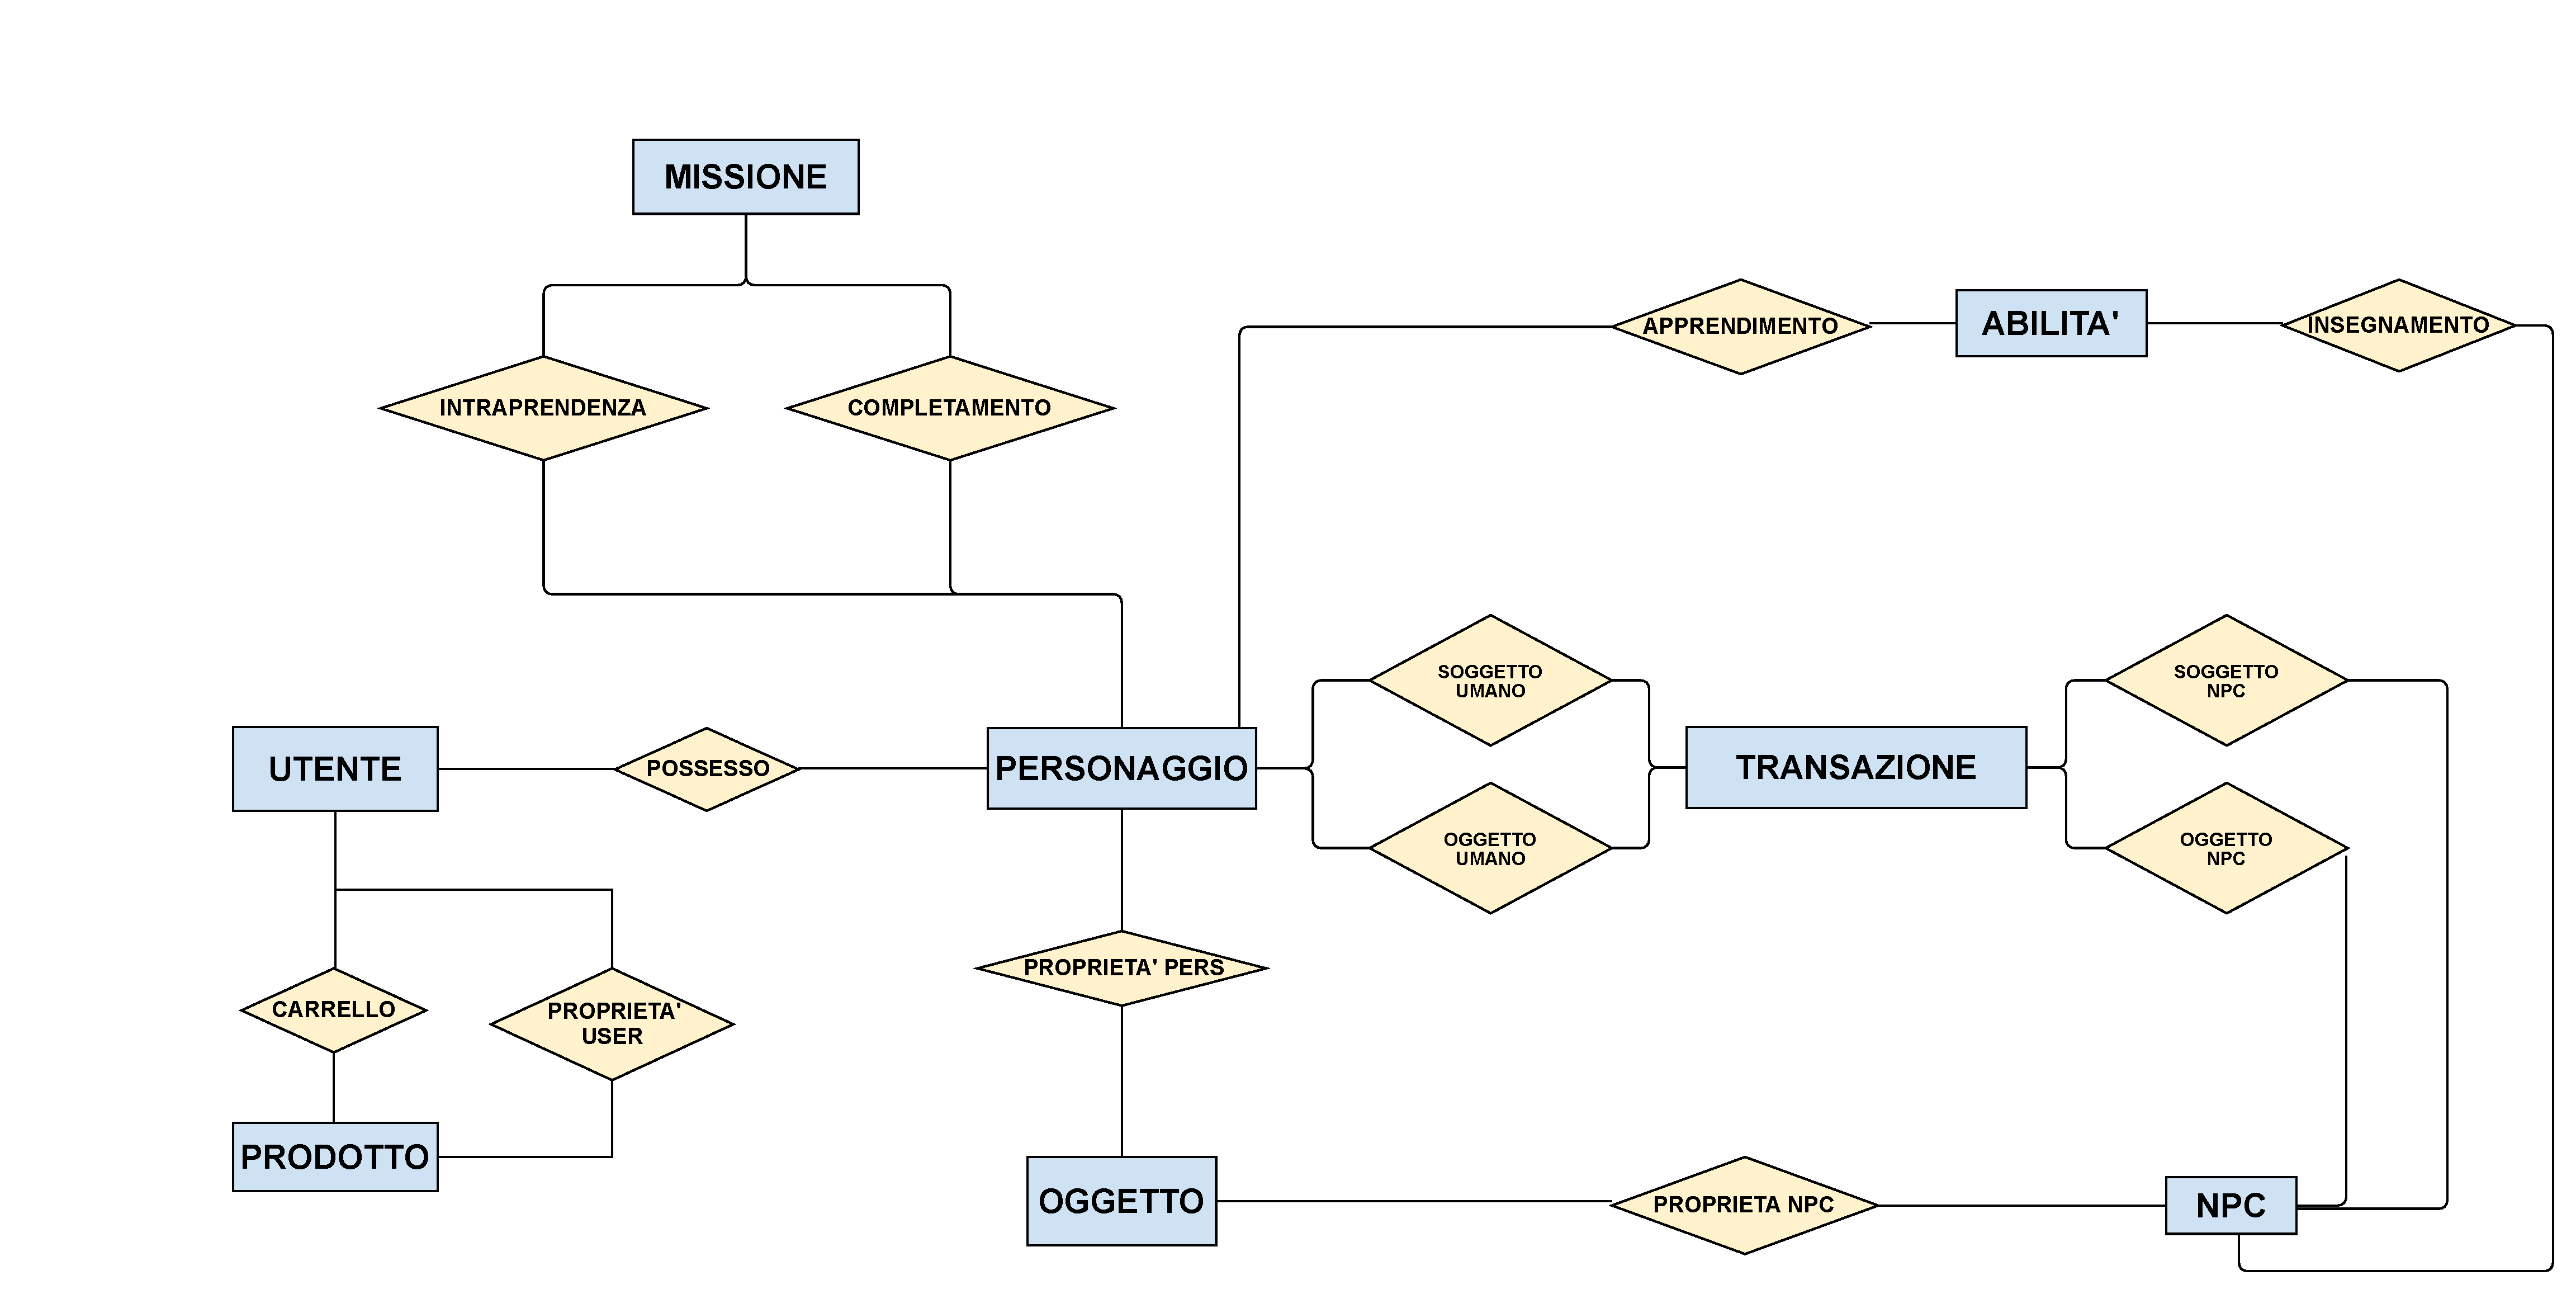
\includegraphics[width=\linewidth]{./immagini/SCHEMASCHELETRO.png}
		\end{figure}

		\end{landscape}

\newpage
		%------------------------------------------------
		\subsection{Sviluppo delle Componenti dello Schema}

		% Procediamo ora secondo la strategia Top-down raffinando le definizioni delle entità e aggiungendo ulteriori relazioni.
% \subsubsection{Personaggio}
% Sappiamo che il personaggio ha parecchie caratteristiche e valori che lo contraddistinguono, possiamo suddividerle in 4 gruppi:
% Posizione, Fisico, Statistiche e Statistiche totali
%
% \begin{figure}[H]
% \centering
% 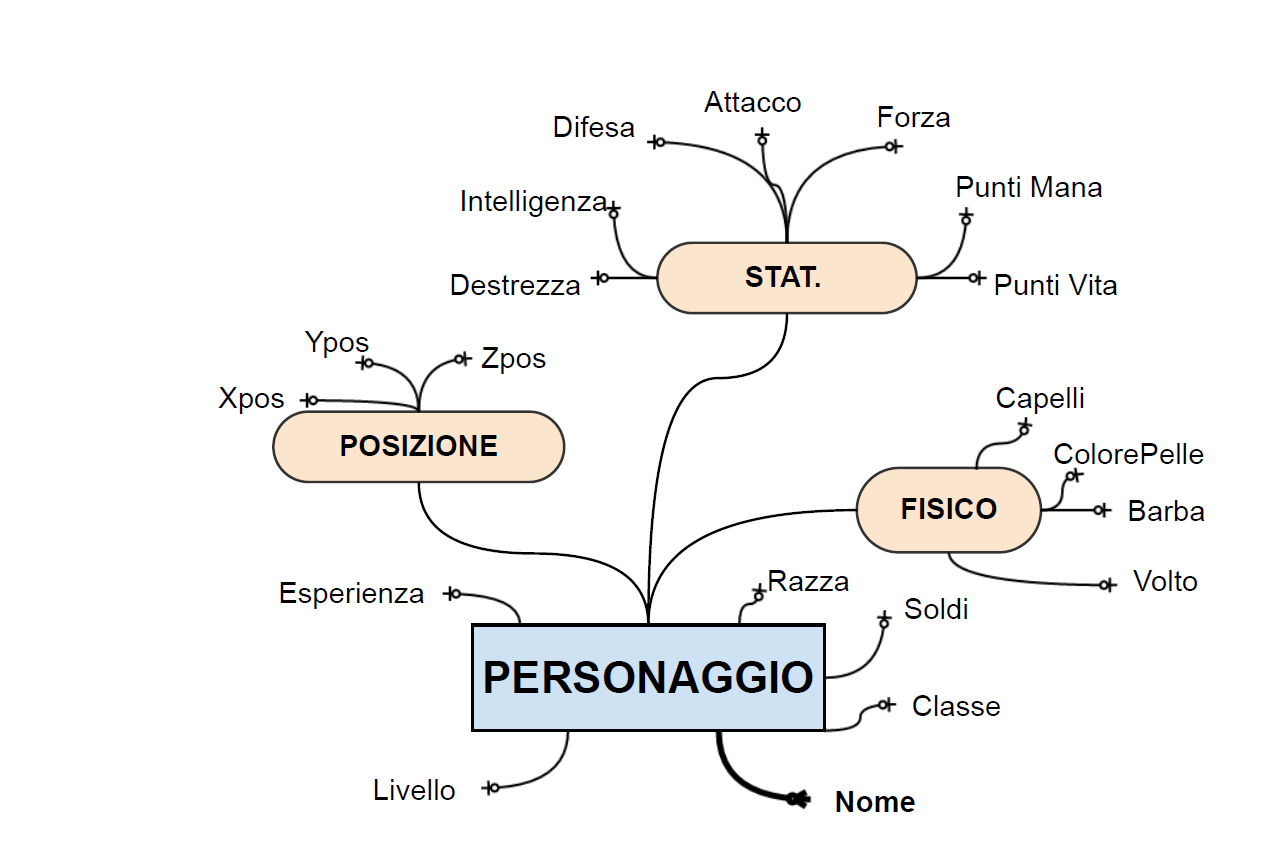
\includegraphics[width=0.7\linewidth]{./immagini/personaggiodef.png}
% \end{figure}
%
% \newpage
%
%
% \subsubsection{NPC}
% Gli npc sono divisi principalmente in ostili e amichevoli, questo ne determina fortemente la funzione all'interno del gioco, le relazioni con le altre entità nonchè i dati stessi che essi utilizzano, è quindi necessaria una Generalizzazione che i suddivida di conseguenza
%
% \begin{figure}[H]
% \centering
% 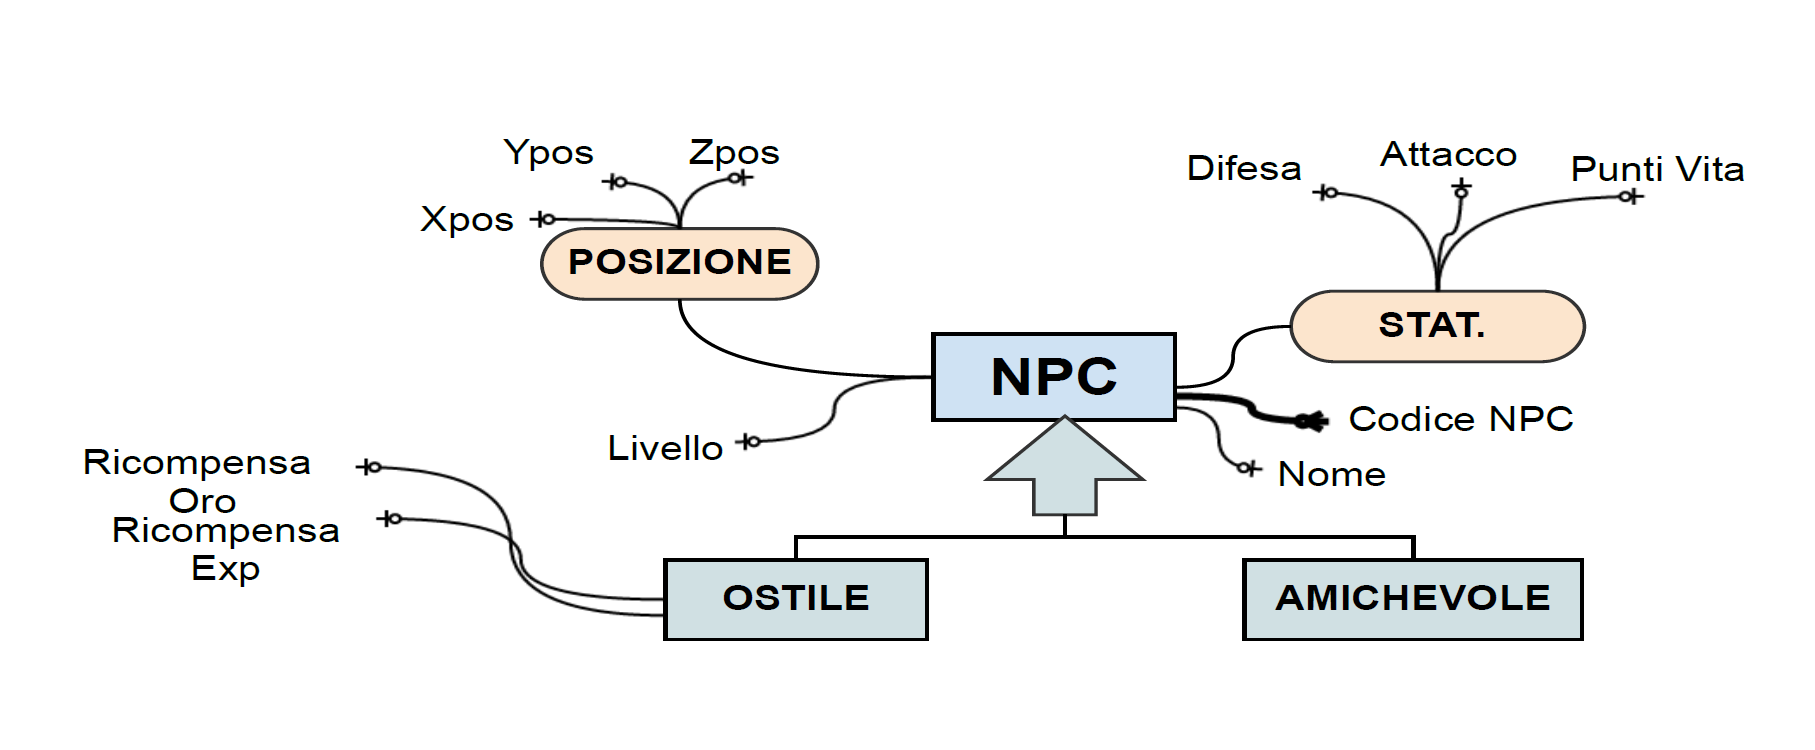
\includegraphics[width=0.7\linewidth]{./immagini/npcdef.png}
% \end{figure}
%
%
% \subsubsection{Oggetto}
% Per gli oggetti sappiamo che alcuni di essi possono essere equipaggiati, consumati dal personeggio oppure essere oggetti missione, questo fatto oltre a comportare una Generalizzazione implica la necessità di una relazione di equipaggiamento, una di consumo e una di stock per descrivere la proprietà di un OGGETTO da parte di un PERSONAGGIO
%
% \begin{figure}[H]
% \centering
% 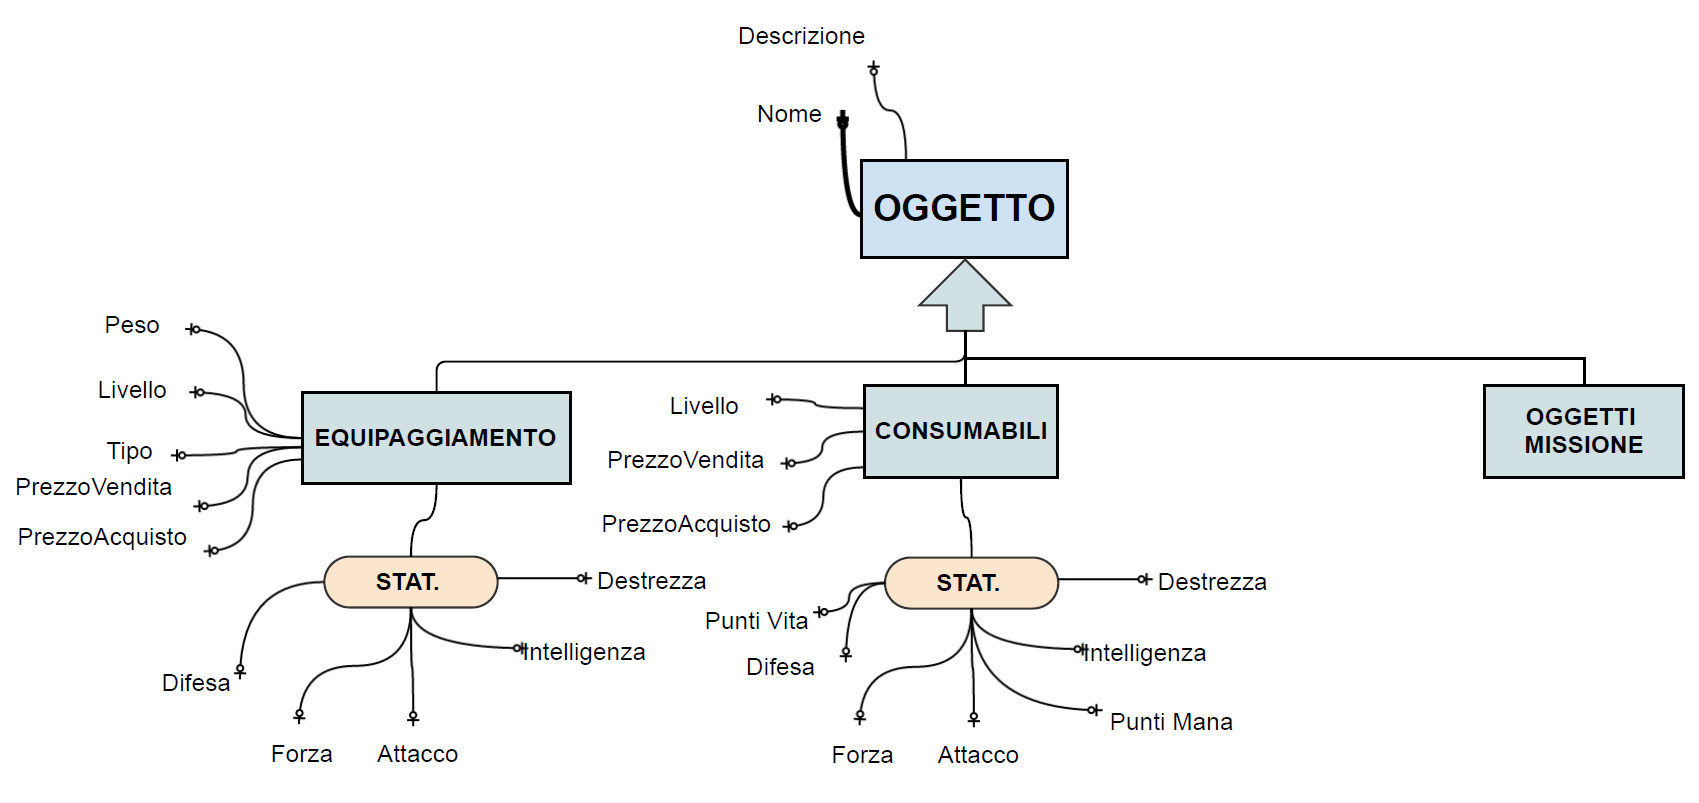
\includegraphics[width=0.7\linewidth]{./immagini/oggettodef.png}
% \end{figure}
%
%  \newpage
%
% \subsubsection{Abilità}
% Dalle interviste sappiamo che le abilità hanno svariati attributi che sono poi i valori da sommare alle statistiche dei personaggi che imparano le abilità, hanno anche un costo e un livello massimo.
%
% \begin{figure}[H]
% \centering
% 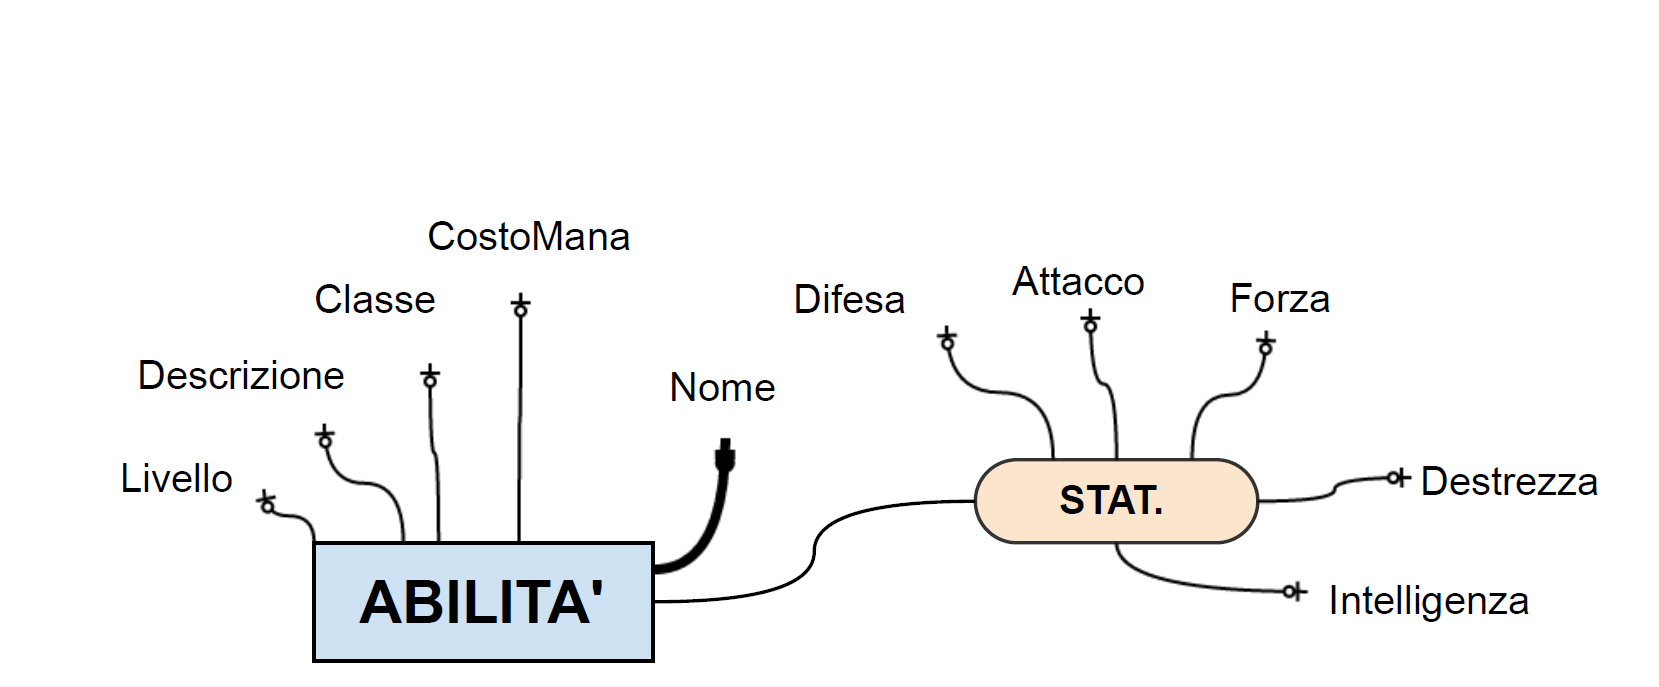
\includegraphics[width=0.7\linewidth]{./immagini/ABILITADEF.png}
% \end{figure}
%
% \subsubsection{Transazione}
% Le transazioni saranno necessarie solo per tenere traccia degli acquisti della sessione, esse avranno un SOGGETTO e un OGGETTO intesi come "chi vende a chi compra"
%
% \begin{figure}[H]
% \centering
% 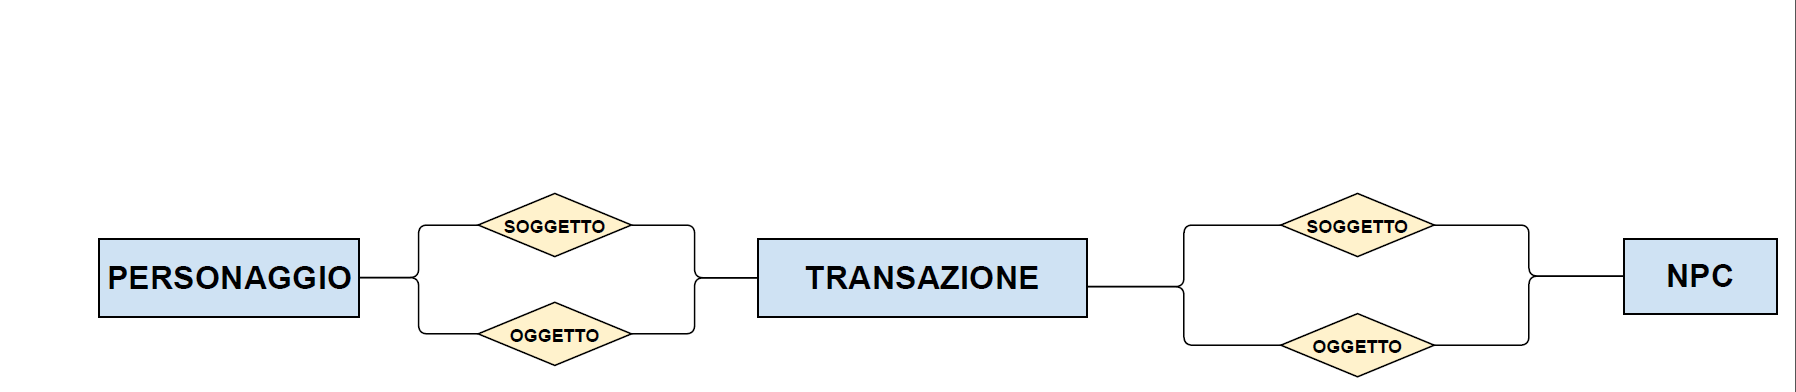
\includegraphics[width=0.7\linewidth]{./immagini/TRANSAZ.png}
% \end{figure}
% AMBIGUITA
%
% \subsubsection{Utente}
% L'utente è la persona vera e propria che si logga per giocare con uno dei suoi personaggi, puo fare acquisti nello Store con una delle sue carte di credito, eliminare o creare personaggi e modificare i suoi dati di fatturazione.
%
%
% \begin{figure}[H]
% \centering
% 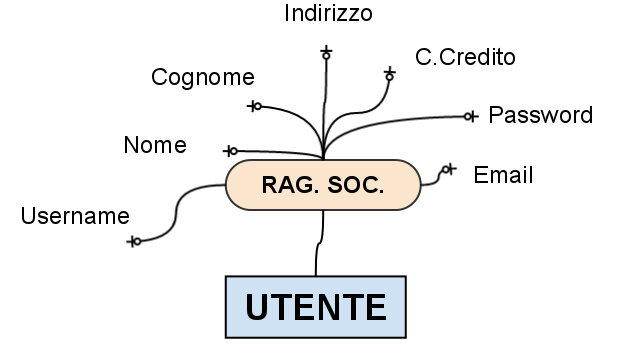
\includegraphics[width=0.7\linewidth]{./immagini/untentedef.png}
% \end{figure}
%
% \subsubsection{Prodotto}
% I PRODOTTI nel nostro gioco sono principalmente 3, cioè le SOTTOSCRIZIONI, I PACCHETTI OGGETTI che permettono di acquistare un gruppo di oggetti Elencati e le ESPANSIONI del Gioco che permettono di raggiungere un livello massimo piu alto.
%
% \begin{figure}[H]
% \centering
% 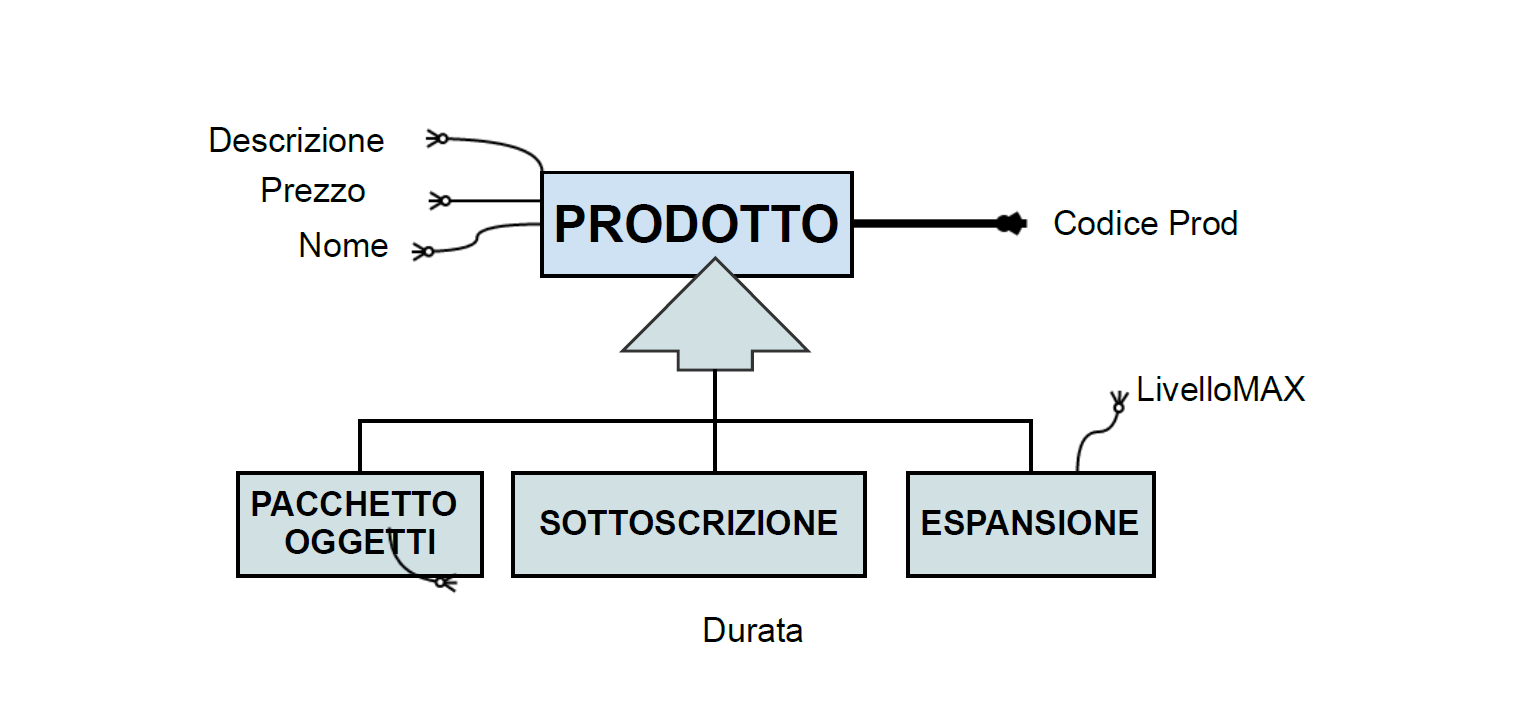
\includegraphics[width=0.7\linewidth]{./immagini/prodottodef.png}
% \end{figure}
%
% \newpage


			\subsubsection{Raffinamenti successivi}

				Per la Relazione di CONSUMO dell'OGGETTO da parte del PERSONAGGIO abbiamo riscontrato un problema, il consumo �  un azione che � possibile ripetere nel corso del tempo per lo stesso oggetto, ci� risulta incompatibile con la nostra definizione di consumo come relazione, � stato quindi necessario Reificare la relazione in un entit� CONSUMO e due relazioni CONSUMANTE e CONSUNTO.

\begin{figure}[H]
\centering
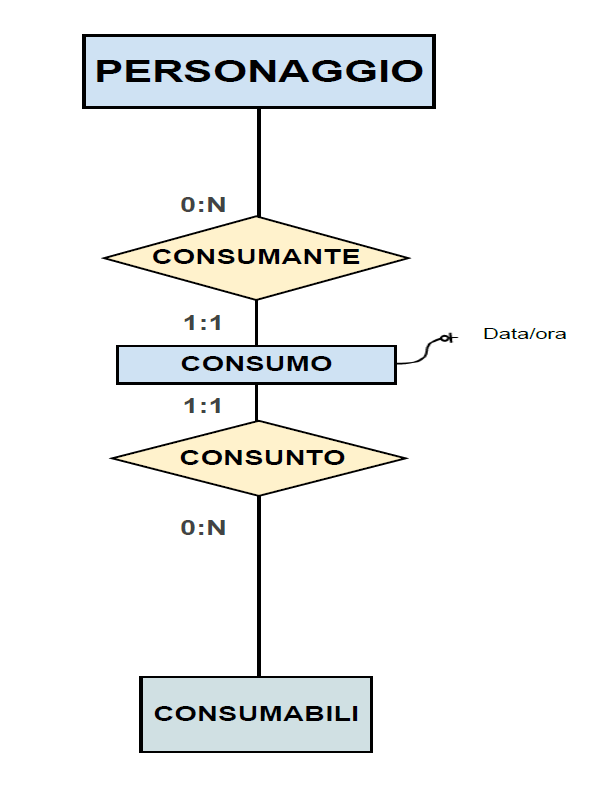
\includegraphics[width=0.4\linewidth]{./immagini/personaggioconsumabili.png}
\end{figure}

\begin{figure}[H]
\centering
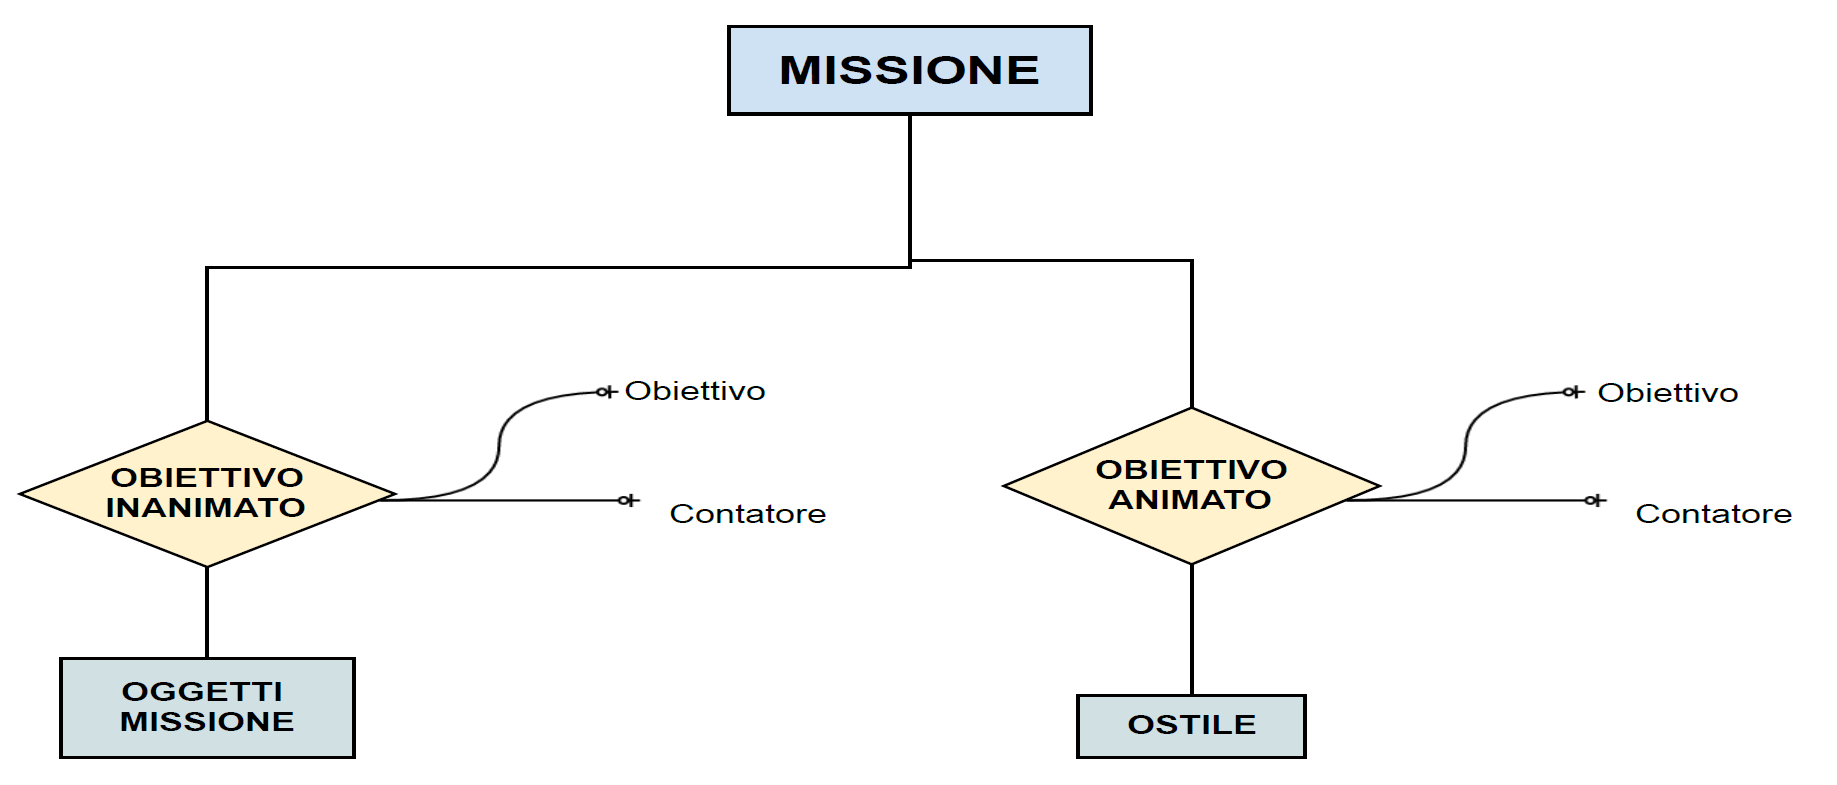
\includegraphics[width=0.8\linewidth]{./immagini/MISSIONEOBIETTIVI.png}
\end{figure}



\begin{landscape} %inizia un foglio landscape

%include un file pdf che contiene lo schema 
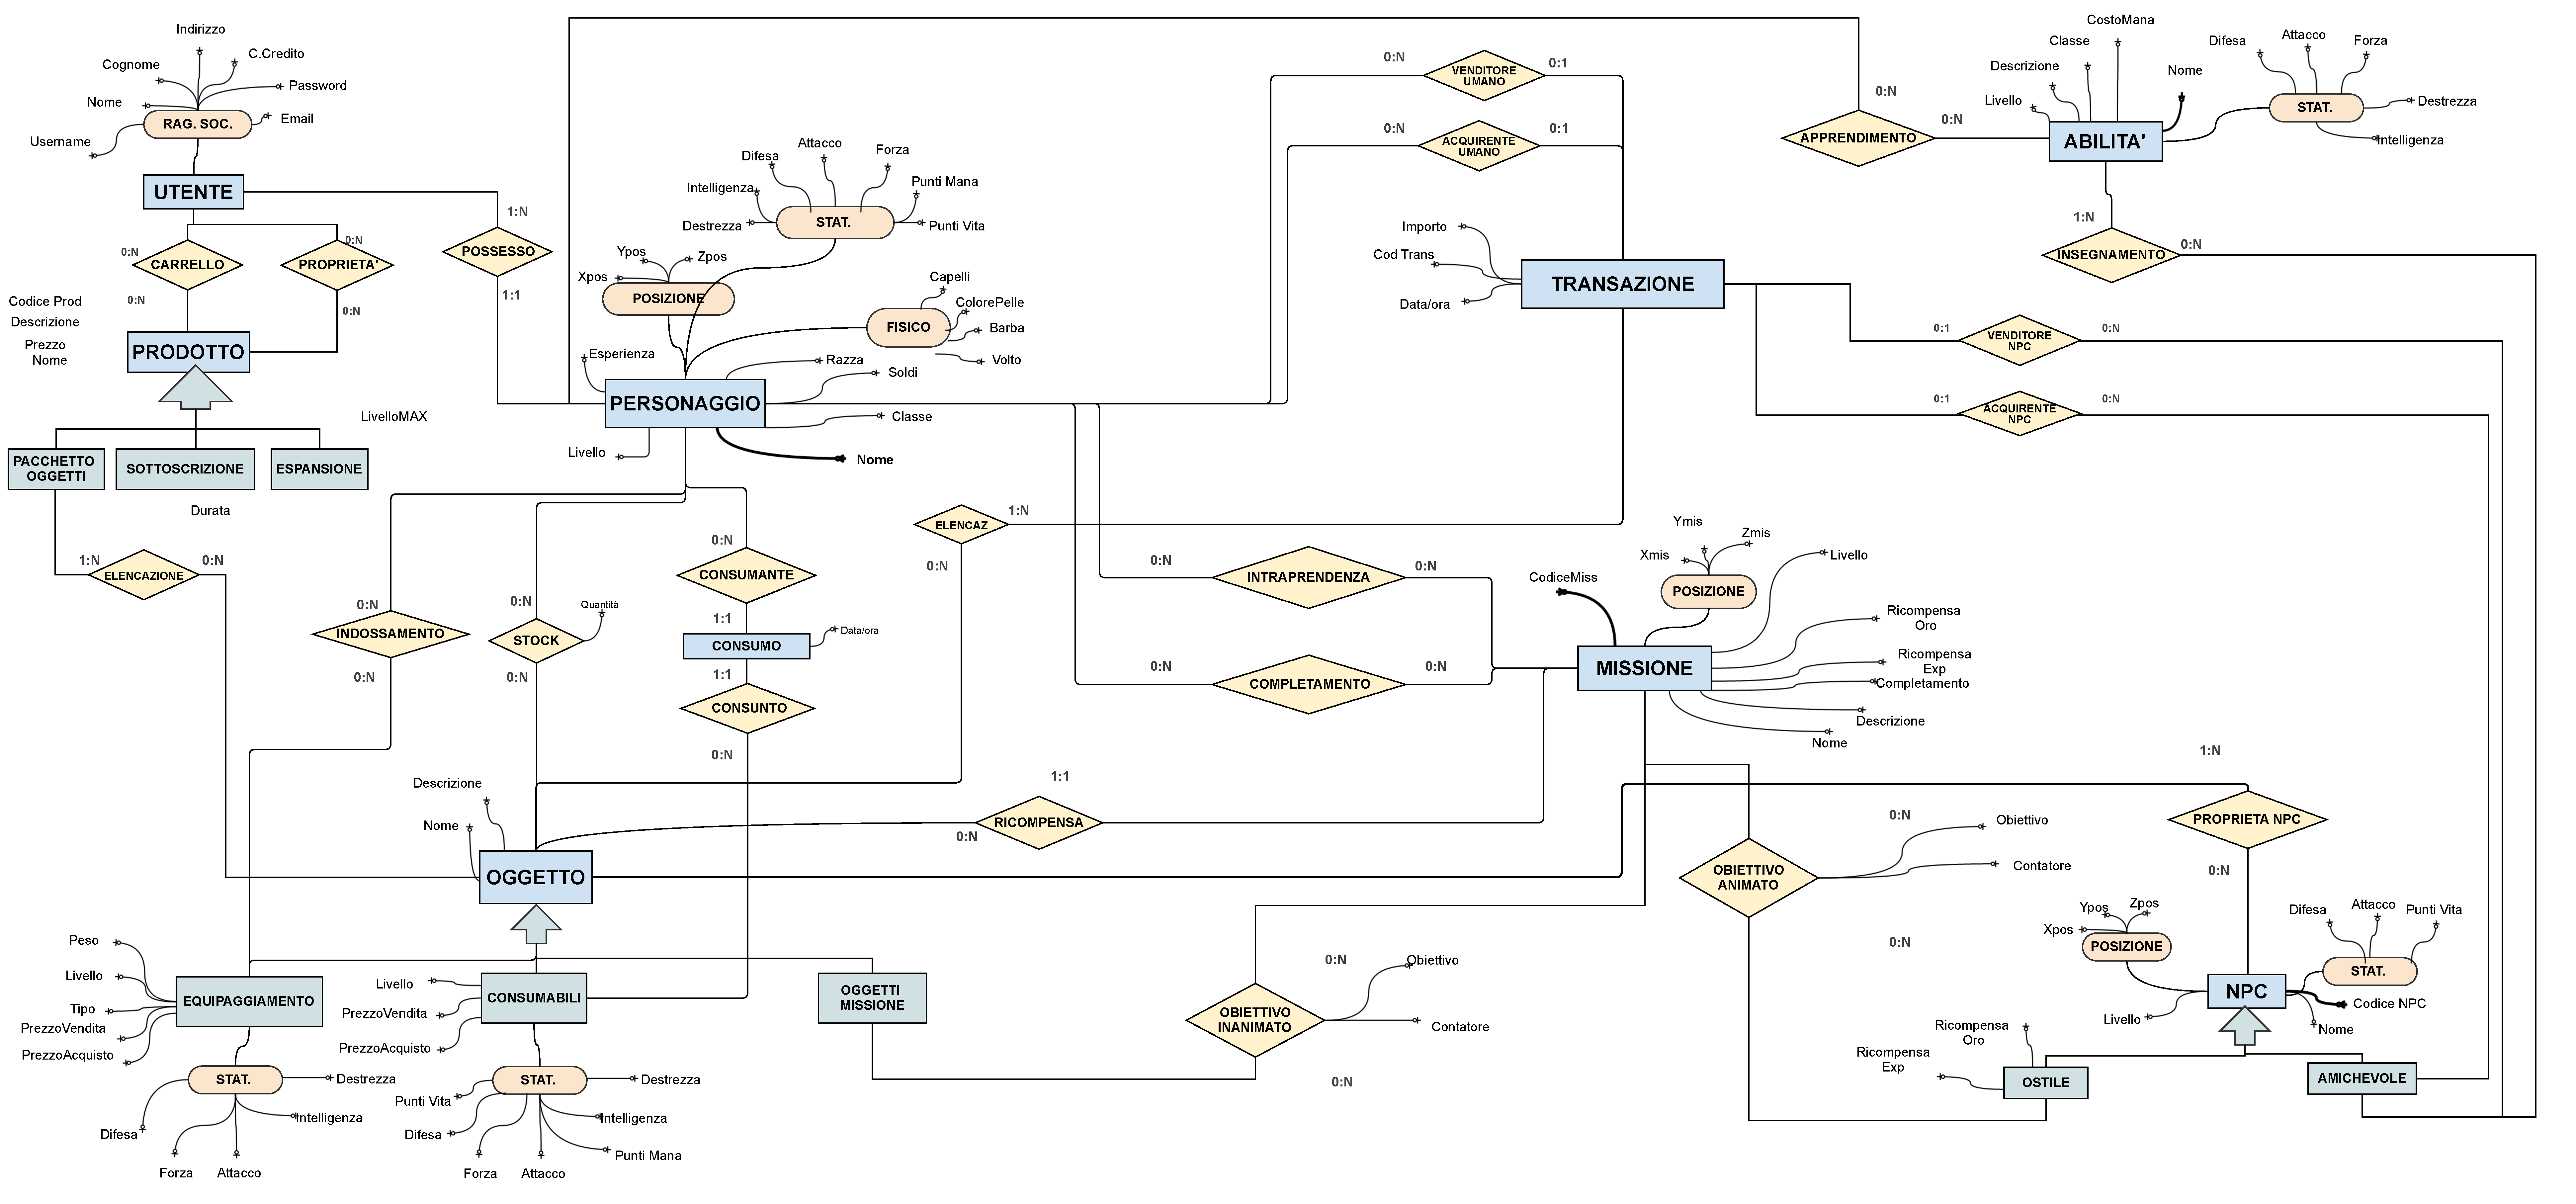
\includepdf[width=270mm, height=210mm, angle=90, keepaspectratio]{./pdf/sbizz.pdf}

\end{landscape}

		%------------------------------------------------
		\subsection{Analisi Qualitativa dello Schema ER}

		In questa fase si effettua un'analisi delle qualità dello schema appena definito. Si suddividono in quattro categorie:
\begin{itemize}
\item \textbf{Correttezza:} Le entità sono usate in maniera consona e congruente per il loro scopo e non risultano errori sintattici e semantici.
\item \textbf{Completezza:} Il flusso di informazioni relativo ai processi interni dell'azienda è ben rappresentato dal modello. Questo significa che lo schema è completo e rappresenta i processi interni in maniera fedele rendendo naturale il percorso logico rappresentato.
\item \textbf{Leggibilità:} Lo schema presenta una buona complessità concentrata maggiormente nella regione centrale. Nonostante ciò il flusso di informazioni risulta spontaneo quindi la comprensibilità dello schema non è compromessa anche se sono stati necessari alcuni incroci per ottimizzare la disposizione di tutti i componenenti.
 \item \textbf{Minimalità:} Ogni specifica è utilizzata una sola volta all'interno dello schema quindi esso non contiene ridondanze.
\end{itemize}


		%------------------------------------------------
		\subsection{Dizionario dei Dati}

			\subsubsection{Entità}

				
\begin{table}[H]
\resizebox{\textwidth}{!}{%
\begin{tabular}{|l|l|l|l|}
\hline
\textbf{Nome Entit�} & \textbf{Descrizione}                                                                                                                                                                             & \textbf{Attributi}                                                                                                                                                                                                                                                                                                                                                                                                                     & \textbf{Identificatore}                                                                                                                                                                                                                                                                                                                  \\ \hline
Utente               & Fruitore finale del gioco                                                                                                                                                                        & \begin{tabular}[c]{@{}l@{}}username (stringa),  nome (stringa), cognome (stringa),\\  indirizzo (stringa), password (stringa), email (stringa)\end{tabular}                                                                                                                                                                                                                                                                            & Username (stringa)                                                                                                                                                                                                                                                                                                                       \\ \hline
Prodotto             & \begin{tabular}[c]{@{}l@{}}Tutto ci� nell'ambito del gioco\\ che l'utente pu� acquistare\\ con valuta reale.\\  Comprende le entit� Sottoscrizione, \\ PacchettoOggetti, Espansione.\end{tabular} & \begin{tabular}[c]{@{}l@{}}Codice (numerico),nome(stringa)\\  descrizione (stringa), prezzo (numerico)\end{tabular}                                                                                                                                                                                                                                                                                                                    & Codice (numerico)                                                                                                                                                                                                                                                                                                                        \\ \hline
Sottoscrizione       & \begin{tabular}[c]{@{}l@{}}� un prodotto, abbonamento mensile\\  del gioco\end{tabular}                                                                                                          & ? Codice (numerico), durata (numerico)                                                                                                                                                                                                                                                                                                                                                                                                 & "                                                                                                                                                                                                                                                                                                                                        \\ \hline
PacchettoOggetti     & \begin{tabular}[c]{@{}l@{}}sono un prodotto, \\ particolari oggetti \\ destinati all'abbellimento\\  del personaggio\end{tabular}                                                                & ? Codice (numerico)                                                                                                                                                                                                                                                                                                                                                                                                                    & "                                                                                                                                                                                                                                                                                                                                        \\ \hline
Espansione           & \begin{tabular}[c]{@{}l@{}}Sono un prodotto, \\ aggiunte al gioco \\ rilasciate a cadenza triennale\\ comprendono nuove missioni e/o \\ nuovi oggetti e/o nuovi NPC\end{tabular}                   & \begin{tabular}[c]{@{}l@{}}??livello massimo? indica il nuovo livello massimo \\ che il personaggio potr� raggiungere.\\ Codice (numerico), livello massimo (numerico)\end{tabular}                                                                                                                                                                                                                                                    & "                                                                                                                                                                                                                                                                                                                                        \\ \hline
Personaggio          & \begin{tabular}[c]{@{}l@{}}Alter ego creato dall'utente\\  per poter giocare\end{tabular}                                                                                                        & \begin{tabular}[c]{@{}l@{}}Nome (stringa), razza (stringa), classe (stringa),\\  livello (numerico), esperienza (numerico), \\ soldi (numerico), capelli (stringa),\\  colorePelle (stringa), barba (stringa), \\ volto (stringa), puntiVita (numerico),\\  puntiMana(numerico), forza (numerico),\\  destrezza (numerico), intelligenza (numerico),\\  xPos (numerico), yPos (numerico), zPos (numerico) nomeUt(stringa)\end{tabular} & \begin{tabular}[c]{@{}l@{}}?razza? � una caratteristica del\\ personaggio e influenza ?classe?\\e le statistiche\\  (?forza?, ?destrezza?, ?intelligenza?).\\ ?capelli?, ?colorePelle?, \\ ?barba?, \\ ?volto? corrispondono ad oggetti \\ grafici del software di gioco.\\ ?xPos?, ?yPos?, ?zPos?\\ cordinate del personaggio\end{tabular} \\ \hline
Transazione          & \begin{tabular}[c]{@{}l@{}}Resoconto degli oggetti acquistati\\ dal personaggio in una sessione di gioco\end{tabular}                                                                            & \begin{tabular}[c]{@{}l@{}}Codice (numerico), dataOra (time), \\ importo (numerico), compratoreReale (stringa),\\  venditoreReale (stringa), compratorePC (stringa),\\  venditorePC (stringa)\end{tabular}                                                                                                                                                                                                                             & \begin{tabular}[c]{@{}l@{}}?dataOra? indica l'orario in cui\\  � stata effettuata la transizione.\\  ?CompratoreReale?,  ?compratorePC?\\ ci dice se chi compra\\  � un personaggio o un NPC.\\  ?venditoreReale?, ?venditorePC? ci dice se\\  chi vende � un personaggio\\ o un NPC\end{tabular}                                            \\ \hline
Consumo              & \begin{tabular}[c]{@{}l@{}}Resoconto degli oggetti\\  consumabili utilizzati dall utente\end{tabular}                                                                                            & Codice ( numerico), data(time)                                                                                                                                                                                                                                                                                                                                                                                                         & ?                                                                                                                                                                                                                                                                                                                                        \\ \hline
Oggetto              & \begin{tabular}[c]{@{}l@{}}Strumenti acquisibili nel gioco.\\  Comprende Equipaggiamento, \\ Consumabili, OggettiMissione\end{tabular}                                                           & Nome (stringa), descrizione (stringa)                                                                                                                                                                                                                                                                                                                                                                                                  & Nome (stringa)                                                                                                                                                                                                                                                                                                                           \\ \hline
Equipaggiamento      & \begin{tabular}[c]{@{}l@{}}Tipologia di oggetto. Strumenti con\\  effetto permanente che influenzano\\  la battaglia.\end{tabular}                                                               & \begin{tabular}[c]{@{}l@{}}nome (stringa), livello ( numerico),\\  tipo (stringa), peso (stringa), attacco (numerico),\\  difesa (numerico), forza(numerico), destrezza (numerico),\\  intelligenza (numerico), prezzoVendita (numerico),\\  prezzoAcquisto(numerico)\end{tabular}                                                                                                                                                     & \begin{tabular}[c]{@{}l@{}}?tipo? specifica se un equipaggiamento \\ � un arma o un armatura.\\ Il ?peso? di un equipaggiamento\\  determina la razza del\\ personaggio che potr� adoperarlo.\end{tabular}                                                                                                                                 \\ \hline
Consumabili          & \begin{tabular}[c]{@{}l@{}}Tipologia di oggetto.\\Strumenti con effetto temporaneo \\ che influenzano la battaglia\end{tabular}                                                                    & \begin{tabular}[c]{@{}l@{}}nome (stringa), livello ( numerico), puntiVita (numerico),\\ puntiMana (numerico), attacco (numerico), difesa (numerico),\\  forza(numerico), destrezza (numerico), intelligenza (numerico),\\  prezzoVendita (numerico), prezzoAcquisto(numerico),durata(intero)\end{tabular}                                                                                                                             &                                                                                                                                                                                                                                                                                                                                          \\ \hline
OggettiMissione      & \begin{tabular}[c]{@{}l@{}}Tipologia di oggetto il cui scopo\\  � il ritrovamento al fine di completare\\  missioni\end{tabular}                                                                 & Nome (stringa)                                                                                                                                                                                                                                                                                                                                                                                                                         & ?                                                                                                                                                                                                                                                                                                                                        \\ \hline
Missione             & \begin{tabular}[c]{@{}l@{}}Incarico che il personaggio svolge\\  per ottenere esperienza e denaro.\end{tabular}                                                                                  & \begin{tabular}[c]{@{}l@{}}Codice (numerico), nome (stringa), descrizione ( stringa), livello (numerico),\\  completamento(numerico),\\  ricompensaOro (numerico), ricompensaExp (numerico),\\  xMiss (numerico), yMiss (numerico), zMiss (numerico)\end{tabular}                                                                                                                                                                      & Codice (numerico)                                                                                                                                                                                                                                                                                                                        \\ \hline
Abilit�              & \begin{tabular}[c]{@{}l@{}}Tecnica di combattimento che\\ il personaggio usa in battaglia.\end{tabular}                                                                                          & \begin{tabular}[c]{@{}l@{}}Nome (stringa), descrizione (stringa), classe (stringa), livello (numerico),\\  costoMana (numerico), \\ attacco (numerico), difesa (numerico), forza(numerico), destrezza (numerico), \\ intelligenza (numerico), prezzo(numerico)\end{tabular}                                                                                                                                                            & Nome (stringa)                                                                                                                                                                                                                                                                                                                           \\ \hline
NPC                  & \begin{tabular}[c]{@{}l@{}}Personaggio gestito dal computer.\\  Si distingue in NPCAmichevole \\ e NPCOstile.\end{tabular}                                                                       & \begin{tabular}[c]{@{}l@{}}Nome (stringa), livello (numerico), puntiVita (numerico), attacco (numerico), \\ difesa (numerico), xPos (numerico), yPos (numerico), zPos (numerico)\end{tabular}                                                                                                                                                                                                                                          & ?                                                                                                                                                                                                                                                                                                                                        \\ \hline
NPCAmichevole        & \begin{tabular}[c]{@{}l@{}}NPC che aiuta il personaggio vendendogli\\ abilit� e oggetti o combattendo\\  al suo fianco\end{tabular}                                                              & ?                                                                                                                                                                                                                                                                                                                                                                                                                                      & ?                                                                                                                                                                                                                                                                                                                                        \\ \hline
NPCOstile            & NPC che combatte contro il personaggio                                                                                                                                                           & \begin{tabular}[c]{@{}l@{}}?\\ Codice (numerico)\end{tabular}                                                                                                                                                                                                                                                                                                                                                                          &                                                                                                                                                                                                                                                                                                                                          \\ \hline
Carta credito        & Elenco delle carte di credito degli utenti                                                                                                                                                       & numero(numerico),cvv(numerico),scadenza(date)                                                                                                                                                                                                                                                                                                                                                                                          &                                                                                                                                                                                                                                                                                                                                          \\ \hline
\end{tabular}
}
\end{table}


		%------------------------------------------------
		\subsection{Regole di Vincolo}

		
\begin{itemize}
\item Gli attributi "Emittente" e "Destinatario" relativi all'entità "Fattura" possono essere "Rimini Service" oppure l'attributo "Nome" di "PA, Persona o Azienda". "Emittente" e "Destinatario" devono essere diversi.
\item "Data scadenza" relativo all'entità "Fattura" deve essere maggiore di "Data emissione" relativo sempre all'entità "Fattura"
\item "Tipologia" relativo a "Servizio" può essere "Riparazione software", "Sostituzione componente", "Configurazione programma", "Formattazione pc", "Installazione rete WiFi"
\item "Colore" relativo alle entità "Cartuccia d'inchiostro" e "Toner" può essere "Nero", "Giallo", "Ciano", "Magenta"
\item "Tecnologia" relativo all'entità "Stampante" può essere "Inkjet" o "Laser"
\item "Formato massimo" relativo all'entità "Stampante" può essere "A3", "A4", "A5"
\item "Connettività" relativo all'entità "Stampante" può essere "USB", "WiFi" o una combinazione di questi
\item "Risoluzione" relativo all'entità "Monitor" può essere "800x600", "1024x768", "1280x720", "1280x800", "1440x900", "1650x1080", "1920x1080", "1920x1200", "2560x1600"
\item "Sistema operativo" relativo alle entità "Pc Desktop" e "Notebook" può essere "Windows 10", "Windows 7", "Mac OS X", "Linux", "Free Dos"
\item "Data termine offerte" relativo all'entità "Richieste sul MEPA" deve essere maggiore di "Data inizio offerte" relativo sempre all'entità "Richieste sul MEPA"
\item "Aggiudicatario" relativo all'entità "Gara pubblica", nel caso la vincitrice della gara sia l'azienda in questione, deve essere "Rimini Service"
\item "Quantità" relativo alle relationship "Stipulazione acquisto" e "Stipulazione vendita" deve essere maggiore di zero.
\item "Prezzo" relativo alla relationship "Catalogo" deve essere maggiore di zero.

\end{itemize}

		%------------------------------------------------
		% \subsection{Vincoli non esprimibili}
    %
		% 
\begin{itemize}
\item Npc non vende a npc
\item Gli Oggetti missione non si vendono
\item Oggetti missione non possono essere ricompense missioni
\item una transazione non puo' avere due relazioni Soggetto o Oggetto
\item La classe \'{e} vincolata alla razza
\end{itemize}

%------------------------------------------------
%
% 	\section{Progettazione Logica}
%
% 		\subsection{Tavola dei Volumi e Delle Operazioni}
%
% 		

\subsubsection{Tavola dei Volumi}

Il gioco in questione \'{e} in fase di progettazione, quindi i volumi delle entit\'{a} e delle relazioni sono stati individuati su una stima di mercato,che prevede il raggiungimento dei valori proposti entro i primi tre mesi di gioco. Solitamente in questo periodo si ha il boom di iscrizioni ad un gioco online, che poi vanno a diminuire di molto nel tempo cos\`{\i}come l'attività dei giocatori. I dati indicati con (**) variano velocemente nel tempo e sono pertanto molto indicativi. 

\begin{table}[H]
\centering

\resizebox{0.7\textwidth}{!}{%
\begin{tabular}{|l|l|l|}
\hline
\textbf{CONCETTO}                & \textbf{TIPO} & \textbf{VOLUME}           \\ \hline
Utente                           & E             & 5000                      \\ \hline
Personaggio                      & E             & 10000                     \\ \hline
Missione                         & E             & 500                       \\ \hline
Abilità                          & E             & 30                        \\ \hline
Oggetto                          & E             & 1000                      \\ \hline
Equipaggiamento                  & E             & 400                       \\ \hline
Consumabili                      & E             & 100                       \\ \hline
Oggetti Missione                 & E             & 500                       \\ \hline
Consumo                          & E             & 100000**                  \\ \hline
Npc Amichevole                   & E             & 750                       \\ \hline
Npc Ostile                       & E             & 1000                      \\ \hline
Transazione                      & E             & 120000**                  \\ \hline
Prodotto                         & E             & 50                        \\ \hline
Sottoscrizione                   & E             & 3                         \\ \hline
Pacchetto Oggetti                & E             & 46                        \\ \hline
Espansione                       & E             & 1                         \\ \hline
Indossamento                     & R             & 14000**                   \\ \hline
Stock                            & R             & 160000                    \\ \hline
Intraprendenza                   & R             & 25000                     \\ \hline
Completamento                    & R             & 10000                     \\ \hline
Obiettivo animato                & R             & 300                       \\ 
\end{tabular}
}
\end{table}
\newpage

\begin{table}[H]
\centering
\resizebox{0.7\textwidth}{!}{%
\begin{tabular}{|l|l|l|}
Obiettivo inanimato              & R             & 400                       \\ \hline
Ricompensa                       & R             & 700                       \\ \hline
Proprietà NPC Amichevole         & R             & 18750                     \\ \hline
Proprietà NPC Ostile             & R             & 4000                      \\ \hline
Apprendimento                    & R             & 50000                     \\ \hline
Insegnamento                     & R             & 5000                      \\ \hline
Possesso                         & R             & 15000                     \\ \hline
Carrello                         & R             & 25000                     \\ \hline
Proprietà                        & R             & 50000                     \\ \hline
Elencazione Pacchetto Oggetti                     & R             & 184  \\ \hline
Elencazione Transazione                          & R             & 120000                          \\ \hline
Consumante                       & R             & 100000**                  \\ \hline
Consunto                         & R             & 100000**                  \\ \hline
Compratore Personaggio           & R             & 90000                           \\ \hline
Venditore Personaggio            & R             & 30000                          \\ \hline
Compratore NPC                   & R             & 30000                          \\ \hline
Venditore NPC                    & R             & 90000                          \\ \hline
Specificazione Sottoscrizione    & R             & 3                         \\ \hline
Specificazione Pacchetto Oggetti & R             & 46                        \\ \hline
Specificazione Espansione        & R             & 1                         \\ \hline
Specificazione Equipaggiamento   & R             & 400                       \\ \hline
Specificazione Consumabili       & R             & 100                       \\ \hline
Specificazione Oggetto Missione  & R             & 500                       \\ \hline
\end{tabular}
}
\end{table}

\subsubsection{Tavola Operazioni}


\begin{table}[H]
\centering
\resizebox{0.5\textwidth}{0.48\textheight}{%
\begin{tabular}{ll}
\hline
\textbf{OPERAZIONE}      & \textbf{FREQUENZA}                           \\ \hline
\multicolumn{1}{|l|}{1}  & \multicolumn{1}{l|}{2 volte al giorno}       \\ \hline
\multicolumn{1}{|l|}{2}  & \multicolumn{1}{l|}{5 volte al giorno}       \\ \hline
\multicolumn{1}{|l|}{3}  & \multicolumn{1}{l|}{175 volta ogni 3 anni}   \\ \hline
\multicolumn{1}{|l|}{4}  & \multicolumn{1}{l|}{200 volte ogni 3 anni}   \\ \hline
\multicolumn{1}{|l|}{5}  & \multicolumn{1}{l|}{100 volte ogni 3 anni}   \\ \hline
\multicolumn{1}{|l|}{6}  & \multicolumn{1}{l|}{35000 volte al giorno}   \\ \hline
\multicolumn{1}{|l|}{7}  & \multicolumn{1}{l|}{21000 volte al giorno}   \\ \hline
\multicolumn{1}{|l|}{8}  & \multicolumn{1}{l|}{10 volte ogni 3 anni}    \\ \hline
\multicolumn{1}{|l|}{9}  & \multicolumn{1}{l|}{2 volte a settimana}     \\ \hline
\multicolumn{1}{|l|}{10} & \multicolumn{1}{l|}{70000 volte al giorno}   \\ \hline
\multicolumn{1}{|l|}{11} & \multicolumn{1}{l|}{200000 volte al giorno}  \\ \hline
\multicolumn{1}{|l|}{12} & \multicolumn{1}{l|}{17500 volte al giorno}   \\ \hline
\multicolumn{1}{|l|}{13} & \multicolumn{1}{l|}{100000 volte al giorno}  \\ \hline
\multicolumn{1}{|l|}{14} & \multicolumn{1}{l|}{87500 volte al giorno}   \\ \hline
\multicolumn{1}{|l|}{15} & \multicolumn{1}{l|}{3750 volte ogni 3 anni}  \\ \hline
\multicolumn{1}{|l|}{16} & \multicolumn{1}{l|}{750 volte ogni 3 anni}   \\ \hline
\multicolumn{1}{|l|}{17} & \multicolumn{1}{l|}{20000 volte ogni 3 anni} \\ \hline
\multicolumn{1}{|l|}{18} & \multicolumn{1}{l|}{250 volte al giorno}     \\ \hline
\multicolumn{1}{|l|}{19} & \multicolumn{1}{l|}{100000 volte al giorno}  \\ \hline
\multicolumn{1}{|l|}{20} & \multicolumn{1}{l|}{87500 volte al giorno}   \\ \hline
\multicolumn{1}{|l|}{21} & \multicolumn{1}{l|}{10 volte ogni 3 anni}    \\ \hline
\multicolumn{1}{|l|}{22} & \multicolumn{1}{l|}{20 volte ogni 3 anni}    \\ \hline
\multicolumn{1}{|l|}{23} & \multicolumn{1}{l|}{10 volte ogni 3 anni}    \\ \hline
\multicolumn{1}{|l|}{24} & \multicolumn{1}{l|}{21000 volte al giorno}   \\ \hline
\multicolumn{1}{|l|}{25} & \multicolumn{1}{l|}{35000 volte al giorno}   \\ \hline
\multicolumn{1}{|l|}{26} & \multicolumn{1}{l|}{3 volte al giorno}       \\ \hline
\multicolumn{1}{|l|}{27} & \multicolumn{1}{l|}{10000 volte al giorno}   \\ \hline
\multicolumn{1}{|l|}{28} & \multicolumn{1}{l|}{17500 volte al giorno}   \\ \hline
\multicolumn{1}{|l|}{29} & \multicolumn{1}{l|}{3500 volte ogni minuto}  \\ \hline
\multicolumn{1}{|l|}{30} & \multicolumn{1}{l|}{175000 volte al giorno}  \\ \hline
\multicolumn{1}{|l|}{31} & \multicolumn{1}{l|}{17500 volte al giorno}   \\ \hline
\multicolumn{1}{|l|}{32} & \multicolumn{1}{l|}{175000 volte al giorno}  \\ \hline
\multicolumn{1}{|l|}{33} & \multicolumn{1}{l|}{175000 volte al giorno}  \\ \hline
\multicolumn{1}{|l|}{34} & \multicolumn{1}{l|}{5 volte ogni mese}       \\ \hline
\multicolumn{1}{|l|}{35} & \multicolumn{1}{l|}{20 volte ogni mese}      \\ \hline
\multicolumn{1}{|l|}{36} & \multicolumn{1}{l|}{1750 volte al giorno}    \\ \hline
\multicolumn{1}{|l|}{37} & \multicolumn{1}{l|}{175000 volte al giorno}  \\ \hline
\multicolumn{1}{|l|}{38} & \multicolumn{1}{l|}{175000 volte al giorno}  \\ \hline
\multicolumn{1}{|l|}{39} & \multicolumn{1}{l|}{175000 volte al giorno}  \\ \hline
\multicolumn{1}{|l|}{40} & \multicolumn{1}{l|}{175000 volte al giorno}  \\ \hline
\multicolumn{1}{|l|}{41} & \multicolumn{1}{l|}{17000 volte al giorno}   \\ \hline
\multicolumn{1}{|l|}{42} & \multicolumn{1}{l|}{35000 volte al giorno}   \\ \hline
\multicolumn{1}{|l|}{43} & \multicolumn{1}{l|}{17000 volte al giorno}   \\ \hline
\multicolumn{1}{|l|}{44} & \multicolumn{1}{l|}{175000 volte al giorno}  \\ \hline
\multicolumn{1}{|l|}{45} & \multicolumn{1}{l|}{175000 volte al giorno}  \\ \hline
\multicolumn{1}{|l|}{46} & \multicolumn{1}{l|}{100000 volte al giorno}  \\ \hline
\end{tabular}
}
\end{table}


% 		%------------------------------------------------
% 		\subsection{Ristrutturazione Schema Concettuale}
%
% 		
\subsubsection{Analisi Derivazioni e Ridondanze}
In questa prima fase analizziamo le ridondanze già presenti. L' unica riscontrata riguarda l'attributo importo ridondante per le entità Contratto di Assistenza on Center e Fattura legate dalla relazione Esecuzione Contratto (operazioni 6, 10, 24, 30, 39), dove l'importo è presente in entrambe le entità.
L'attributo importo nell'entità Fattura è vincolato dalla decisione di non conservare tutti i cataloghi dei fornitori per questioni di spazio. Quindi aggiornando mensilmente i prezzi dei cataloghi si perde la possibilità di andare a cercare il valore di un prodotto in un certo arco temporale se non quello attuale, e questo renderebbe impossibile calcolare l'importo di una fattura a posteriori. Per questo motivo l'attributo importo deve essere presente e lo si considera ridondante nell'entità del contratto di assistenza on center piuttosto che nella fattura.
\newline\newline
\centerline{\textbf{ATTRIBUTO IMPORTO IN CONTRATTO DI ASSISTENZA ON CENTER}}
\newline
\centerline{\textbf{CON RIDONDANZA}}
\begin{table}[H]
\centering
\caption{Operazione 6}
\begin{tabular}{llll}
\\ \hline
\multicolumn{1}{|l|}{\textbf{CONCETTO}} & \multicolumn{1}{l|}{\textbf{COSTRUTTO}} & \multicolumn{1}{l|}{\textbf{ACCESSI}} & \multicolumn{1}{l|}{\textbf{TIPO}} \\ \hline
\multicolumn{1}{|l|}{FATTURA}
& \multicolumn{1}{l|}{E}                  & \multicolumn{1}{l|}{1}                & \multicolumn{1}{l|}{S}             \\ \hline
\end{tabular}
\end{table}


\begin{table}[H]
\centering
\caption{Operazione 10}
\begin{tabular}{llll}
\\ \hline
\multicolumn{1}{|l|}{\textbf{CONCETTO}} & \multicolumn{1}{l|}{\textbf{COSTRUTTO}} & \multicolumn{1}{l|}{\textbf{ACCESSI}} & \multicolumn{1}{l|}{\textbf{TIPO}} \\ \hline
\multicolumn{1}{|l|}{Contratto di assistenza on center}
& \multicolumn{1}{l|}{E}                  & \multicolumn{1}{l|}{1}                & \multicolumn{1}{l|}{L}             \\ \hline
\multicolumn{1}{|l|}{Fattura}             & \multicolumn{1}{l|}{E}                  & \multicolumn{1}{l|}{1}                & \multicolumn{1}{l|}{L}             \\ \hline
\multicolumn{1}{|l|}{Esecuzione Contratto}     & \multicolumn{1}{l|}{R}                  & \multicolumn{1}{l|}{2}                & \multicolumn{1}{l|}{S}             \\ \hline
\multicolumn{1}{|l|}{Esecuzione Contratto}
& \multicolumn{1}{l|}{R}                  & \multicolumn{1}{l|}{2}                & \multicolumn{1}{l|}{L}             \\ \hline
\end{tabular}
\end{table}

\begin{table}[H]
\centering
\caption{Operazione 24}
\begin{tabular}{llll}
\\ \hline
\multicolumn{1}{|l|}{\textbf{CONCETTO}} & \multicolumn{1}{l|}{\textbf{COSTRUTTO}} & \multicolumn{1}{l|}{\textbf{ACCESSI}} & \multicolumn{1}{l|}{\textbf{TIPO}} \\ \hline
\multicolumn{1}{|l|}{Esecuzione Contratto}
& \multicolumn{1}{l|}{R}                  & \multicolumn{1}{l|}{1}                & \multicolumn{1}{l|}{L}             \\ \hline
\end{tabular}
\end{table}

\begin{table}[H]
\centering
\caption{Operazione 25}
\begin{tabular}{llll}
\\ \hline
\multicolumn{1}{|l|}{\textbf{CONCETTO}} & \multicolumn{1}{l|}{\textbf{COSTRUTTO}} & \multicolumn{1}{l|}{\textbf{ACCESSI}} & \multicolumn{1}{l|}{\textbf{TIPO}} \\ \hline
\multicolumn{1}{|l|}{Esecuzione Contratto}
& \multicolumn{1}{l|}{R}                  & \multicolumn{1}{l|}{1*1=1}                & \multicolumn{1}{l|}{L}             \\ \hline
\end{tabular}
\end{table}

\begin{table}[H]
\centering
\caption{Operazione 30}
\begin{tabular}{llll}
\\ \hline
\multicolumn{1}{|l|}{\textbf{CONCETTO}} & \multicolumn{1}{l|}{\textbf{COSTRUTTO}} & \multicolumn{1}{l|}{\textbf{ACCESSI}} & \multicolumn{1}{l|}{\textbf{TIPO}} \\ \hline
\multicolumn{1}{|l|}{Fattura}
& \multicolumn{1}{l|}{E}                  & \multicolumn{1}{l|}{1}                & \multicolumn{1}{l|}{L}             \\ \hline
\end{tabular}
\end{table}

\begin{table}[H]
\centering
\caption{Operazione 39}
\begin{tabular}{llll}
\\ \hline
\multicolumn{1}{|l|}{\textbf{CONCETTO}} & \multicolumn{1}{l|}{\textbf{COSTRUTTO}} & \multicolumn{1}{l|}{\textbf{ACCESSI}} & \multicolumn{1}{l|}{\textbf{TIPO}} \\ \hline
\multicolumn{1}{|l|}{Fattura}
& \multicolumn{1}{l|}{R}                  & \multicolumn{1}{l|}{1*12=12}                & \multicolumn{1}{l|}{L}             \\ \hline
\end{tabular}
\end{table}


\newline\newline\centerline{\textbf{SENZA RIDONDANZA}}
\begin{table}[H]
\centering
\caption{Operazione 6}
\begin{tabular}{llll}
\\ \hline
\multicolumn{1}{|l|}{\textbf{CONCETTO}} & \multicolumn{1}{l|}{\textbf{COSTRUTTO}} & \multicolumn{1}{l|}{\textbf{ACCESSI}} & \multicolumn{1}{l|}{\textbf{TIPO}} \\ \hline
\multicolumn{1}{|l|}{FATTURA}
& \multicolumn{1}{l|}{E}                  & \multicolumn{1}{l|}{1}                & \multicolumn{1}{l|}{S}             \\ \hline
\end{tabular}
\end{table}


\begin{table}[H]
\centering
\caption{Operazione 10}
\begin{tabular}{llll}
\\ \hline
\multicolumn{1}{|l|}{\textbf{CONCETTO}} & \multicolumn{1}{l|}{\textbf{COSTRUTTO}} & \multicolumn{1}{l|}{\textbf{ACCESSI}} & \multicolumn{1}{l|}{\textbf{TIPO}} \\ \hline
\multicolumn{1}{|l|}{Fattura}             & \multicolumn{1}{l|}{E}                  & \multicolumn{1}{l|}{1}                & \multicolumn{1}{l|}{L}             \\ \hline
\multicolumn{1}{|l|}{Esecuzione Contratto}     & \multicolumn{1}{l|}{R}                  & \multicolumn{1}{l|}{1}                & \multicolumn{1}{l|}{S}             \\ \hline
\multicolumn{1}{|l|}{Esecuzione Contratto}
& \multicolumn{1}{l|}{R}                  & \multicolumn{1}{l|}{1}                & \multicolumn{1}{l|}{L}             \\ \hline
\end{tabular}
\end{table}

\begin{table}[H]
\centering
\caption{Operazione 24}
\begin{tabular}{llll}
\\ \hline
\multicolumn{1}{|l|}{\textbf{CONCETTO}} & \multicolumn{1}{l|}{\textbf{COSTRUTTO}} & \multicolumn{1}{l|}{\textbf{ACCESSI}} & \multicolumn{1}{l|}{\textbf{TIPO}} \\ \hline
\multicolumn{1}{|l|}{Esecuzione Contratto}
& \multicolumn{1}{l|}{R}                  & \multicolumn{1}{l|}{1}                & \multicolumn{1}{l|}{L}             \\ \hline
\multicolumn{1}{|l|}{Fattura}             & \multicolumn{1}{l|}{E}                  & \multicolumn{1}{l|}{1}                & \multicolumn{1}{l|}{L}             \\ \hline
\end{tabular}
\end{table}

\begin{table}[H]
\centering
\caption{Operazione 25}
\begin{tabular}{llll}
\\ \hline
\multicolumn{1}{|l|}{\textbf{CONCETTO}} & \multicolumn{1}{l|}{\textbf{COSTRUTTO}} & \multicolumn{1}{l|}{\textbf{ACCESSI}} & \multicolumn{1}{l|}{\textbf{TIPO}} \\ \hline
\multicolumn{1}{|l|}{Esecuzione Contratto}
& \multicolumn{1}{l|}{R}                  & \multicolumn{1}{l|}{1*1=1}                & \multicolumn{1}{l|}{L}             \\ \hline
\multicolumn{1}{|l|}{Fattura}             & \multicolumn{1}{l|}{E}                  & \multicolumn{1}{l|}{1*1=1}                & \multicolumn{1}{l|}{L}             \\ \hline
\end{tabular}
\end{table}

\begin{table}[H]
\centering
\caption{Operazione 30}
\begin{tabular}{llll}
\\ \hline
\multicolumn{1}{|l|}{\textbf{CONCETTO}} & \multicolumn{1}{l|}{\textbf{COSTRUTTO}} & \multicolumn{1}{l|}{\textbf{ACCESSI}} & \multicolumn{1}{l|}{\textbf{TIPO}} \\ \hline
\multicolumn{1}{|l|}{Fattura}
& \multicolumn{1}{l|}{E}                  & \multicolumn{1}{l|}{1}                & \multicolumn{1}{l|}{L}             \\ \hline
\end{tabular}
\end{table}

\begin{table}[H]
\centering
\caption{Operazione 39}
\begin{tabular}{llll}
\\ \hline
\multicolumn{1}{|l|}{\textbf{CONCETTO}} & \multicolumn{1}{l|}{\textbf{COSTRUTTO}} & \multicolumn{1}{l|}{\textbf{ACCESSI}} & \multicolumn{1}{l|}{\textbf{TIPO}} \\ \hline
\multicolumn{1}{|l|}{Fattura}
& \multicolumn{1}{l|}{R}                  & \multicolumn{1}{l|}{1*12=12}                & \multicolumn{1}{l|}{L}             \\ \hline
\end{tabular}
\end{table}


\begin{table}[H]
\centering
\caption{Costo Operazioni con ridondanza}
\label{my-label}
\resizebox{\textwidth}{!}{%
\begin{tabular}{|l|l|l|l|}
\hline
\textbf{OPERAZIONE}               & \textbf{COSTO} & \textbf{FREQUENZA} & \textbf{TOTALE} \\ \hline
6                                & 1             & 90             & 90
\\ \hline
10                                & 6              & 1              & 6
\\ \hline
24                                & 1              & 8             & 8
\\ \hline
25                                & 1              & 2              & 2
\\ \hline
30                                & 1              & 30             & 30
\\ \hline
39                                & 12             & 1             & 12
\\ \hline
COSTO OPERAZIONI CON RIDONDANZA & 22        &                    &   \hl{148}             \\ \hline
\end{tabular}
}
\end{table}


\begin{table}[H]
\centering
\caption{Costo Operazioni senza Ridondanza}
\label{my-label}
\resizebox{\textwidth}{!}{%
\begin{tabular}{|l|l|l|l|}
\hline
\textbf{OPERAZIONE}             & \textbf{COSTO} & \textbf{FREQUENZA} & \textbf{TOTALE} \\ \hline
6                                & 1             & 90             & 90
\\ \hline
10                                & 3              & 1              & 3
\\ \hline
24                                & 2              & 8             & 16
\\ \hline
25                                & 2              & 2              & 4
\\ \hline
30                                & 1              & 30             & 30          \\ \hline
39                                & 12             & 1             & 12
\\ \hline
COSTO OPERAZIONI SENZA RIDONDANZA & 21        &                    &  \hl{155}               \\ \hline
\end{tabular}
}
\end{table}
Dai calcoli effettuati risulta evidente una differenza davvero minima per quanto concerne il costo delle operazioni. In questo caso si sceglie di non rindondare l'attributo, per avere un guadagno di memoria, al prezzo di qualche operazioni in più.
\newline
Inoltre dall'analisi del modello non è stata riscontrata la possibilità di inserire ulteriori attributi ridondanti.


\newpage
\subsubsection{Eliminazione Delle Gerarchie}

Nel nostro schema concettuale sono presenti 5 generalizzazioni. Le Entità coinvolte sono "PA, Azienda o Persona", "Cliente", "Richiesta sul Mepa", "Prodotto o servizio", "Prodotto".
\newline
Abbiamo deciso di procedere nel seguente modo:

\paragraph{PA, Azienda o Persona}
Per quanto riguarda l'entità PA, Azienda o Persona, abbiamo scelto di accorpare il genitore della generalizzazione nelle entità figlie. Questo perchè i clienti e i fornitori hanno rapporti con l'azienda piuttosto diversi tra loro, quindi la separazione comporta una suddivisione concettuale che migliora la chiarezza dello schema.
\paragraph{Cliente}
Per l'entità Cliente si è adottata una soluzione ibrida. Abbiamo optato di mantenere il genitore l'entità figlia Pubblica Amministrazione, mentre l'entità Privato è stata accorpata nel genitore aggiungendo un nuovo attributo "Tipo", che indica appunto se il Cliente è un Privato o una PA. Un eventuale accorpamento del genitore nelle entità figlie avrebbe complicato lo schema, viste le numerose relazioni che ha il genitore.
\newline
La relazione tra Cliente e PA è denominata "Specificazione PA".
\paragraph{Richiesta sul Mepa}
In merito all'entità Richiesta sul Mepa, si è deciso di sostituire la generalizzazione con delle relazioni. Si avrebbe potuto accorpare le entità figlie nel genitore, utilizzando degli attributi che possono assumere il valore NULL per poter distinguire appunto le due entità, ma ci sembra più opportuno mantenere distinte le entità Gara pubblica e Trattativa diretta in quanto esse sono, nella realtà pratica, due concetti logicamente separati.
Le nuove relazioni sono denominate "Specificazione gara" e "Specificazione trattativa".
\paragraph{Prodotto o Servizio}
Anche con l'entità Prodotto o Servizio abbiamo scelto di mantenere il genitore e le entità figlie, sostituendo la generalizzazione con delle relazioni. Le nuove relazioni sono "Specificazione prodotto" e "Specificazione Servizio".
\paragraph{Prodotto}
Per l'entità Prodotto si è scelto di mantenere sia il padre che le entità figlie, dato che queste ultime hanno tanti attributi diversi, e l'accorpamento nell'entità genitore significherebbe avere tanti valori con valore NULL. Inoltre, un eventuale accorpamento del genitore nelle entità figlie risulterebbe piuttosto complicato, date le numerose relazioni che ha il padre e visto che le entità figlie sono molteplici.
Quindi, si è scelto di sostituire la generalizzazione con delle relazioni, una per ogni entità figlia. Le nuove relazioni sono denominate "Specificazione" più il nome dell'entità a cui si riferiscono.
\newline\newline
In seguito all'aggiunta dell'attributo "Tipo" all'entità "Cliente", è necessario introdurre una nuova regola di vincolo:

\begin{itemize}
  \item L'attributo "Tipo" relativo all'entità "Cliente" può essere "Privato" oppure "PA".
\end{itemize}
\noindent
\textit{(Facciamo notare che, per non appesantire ulteriormente lo schema, abbiamo scelto di togliere alcuni prodotti e di mantenere solo "Notebook", "Pc Desktop", "Monitor", "Stampante".)}



\newpage
\begin{landscape} %inizia un foglio landscape

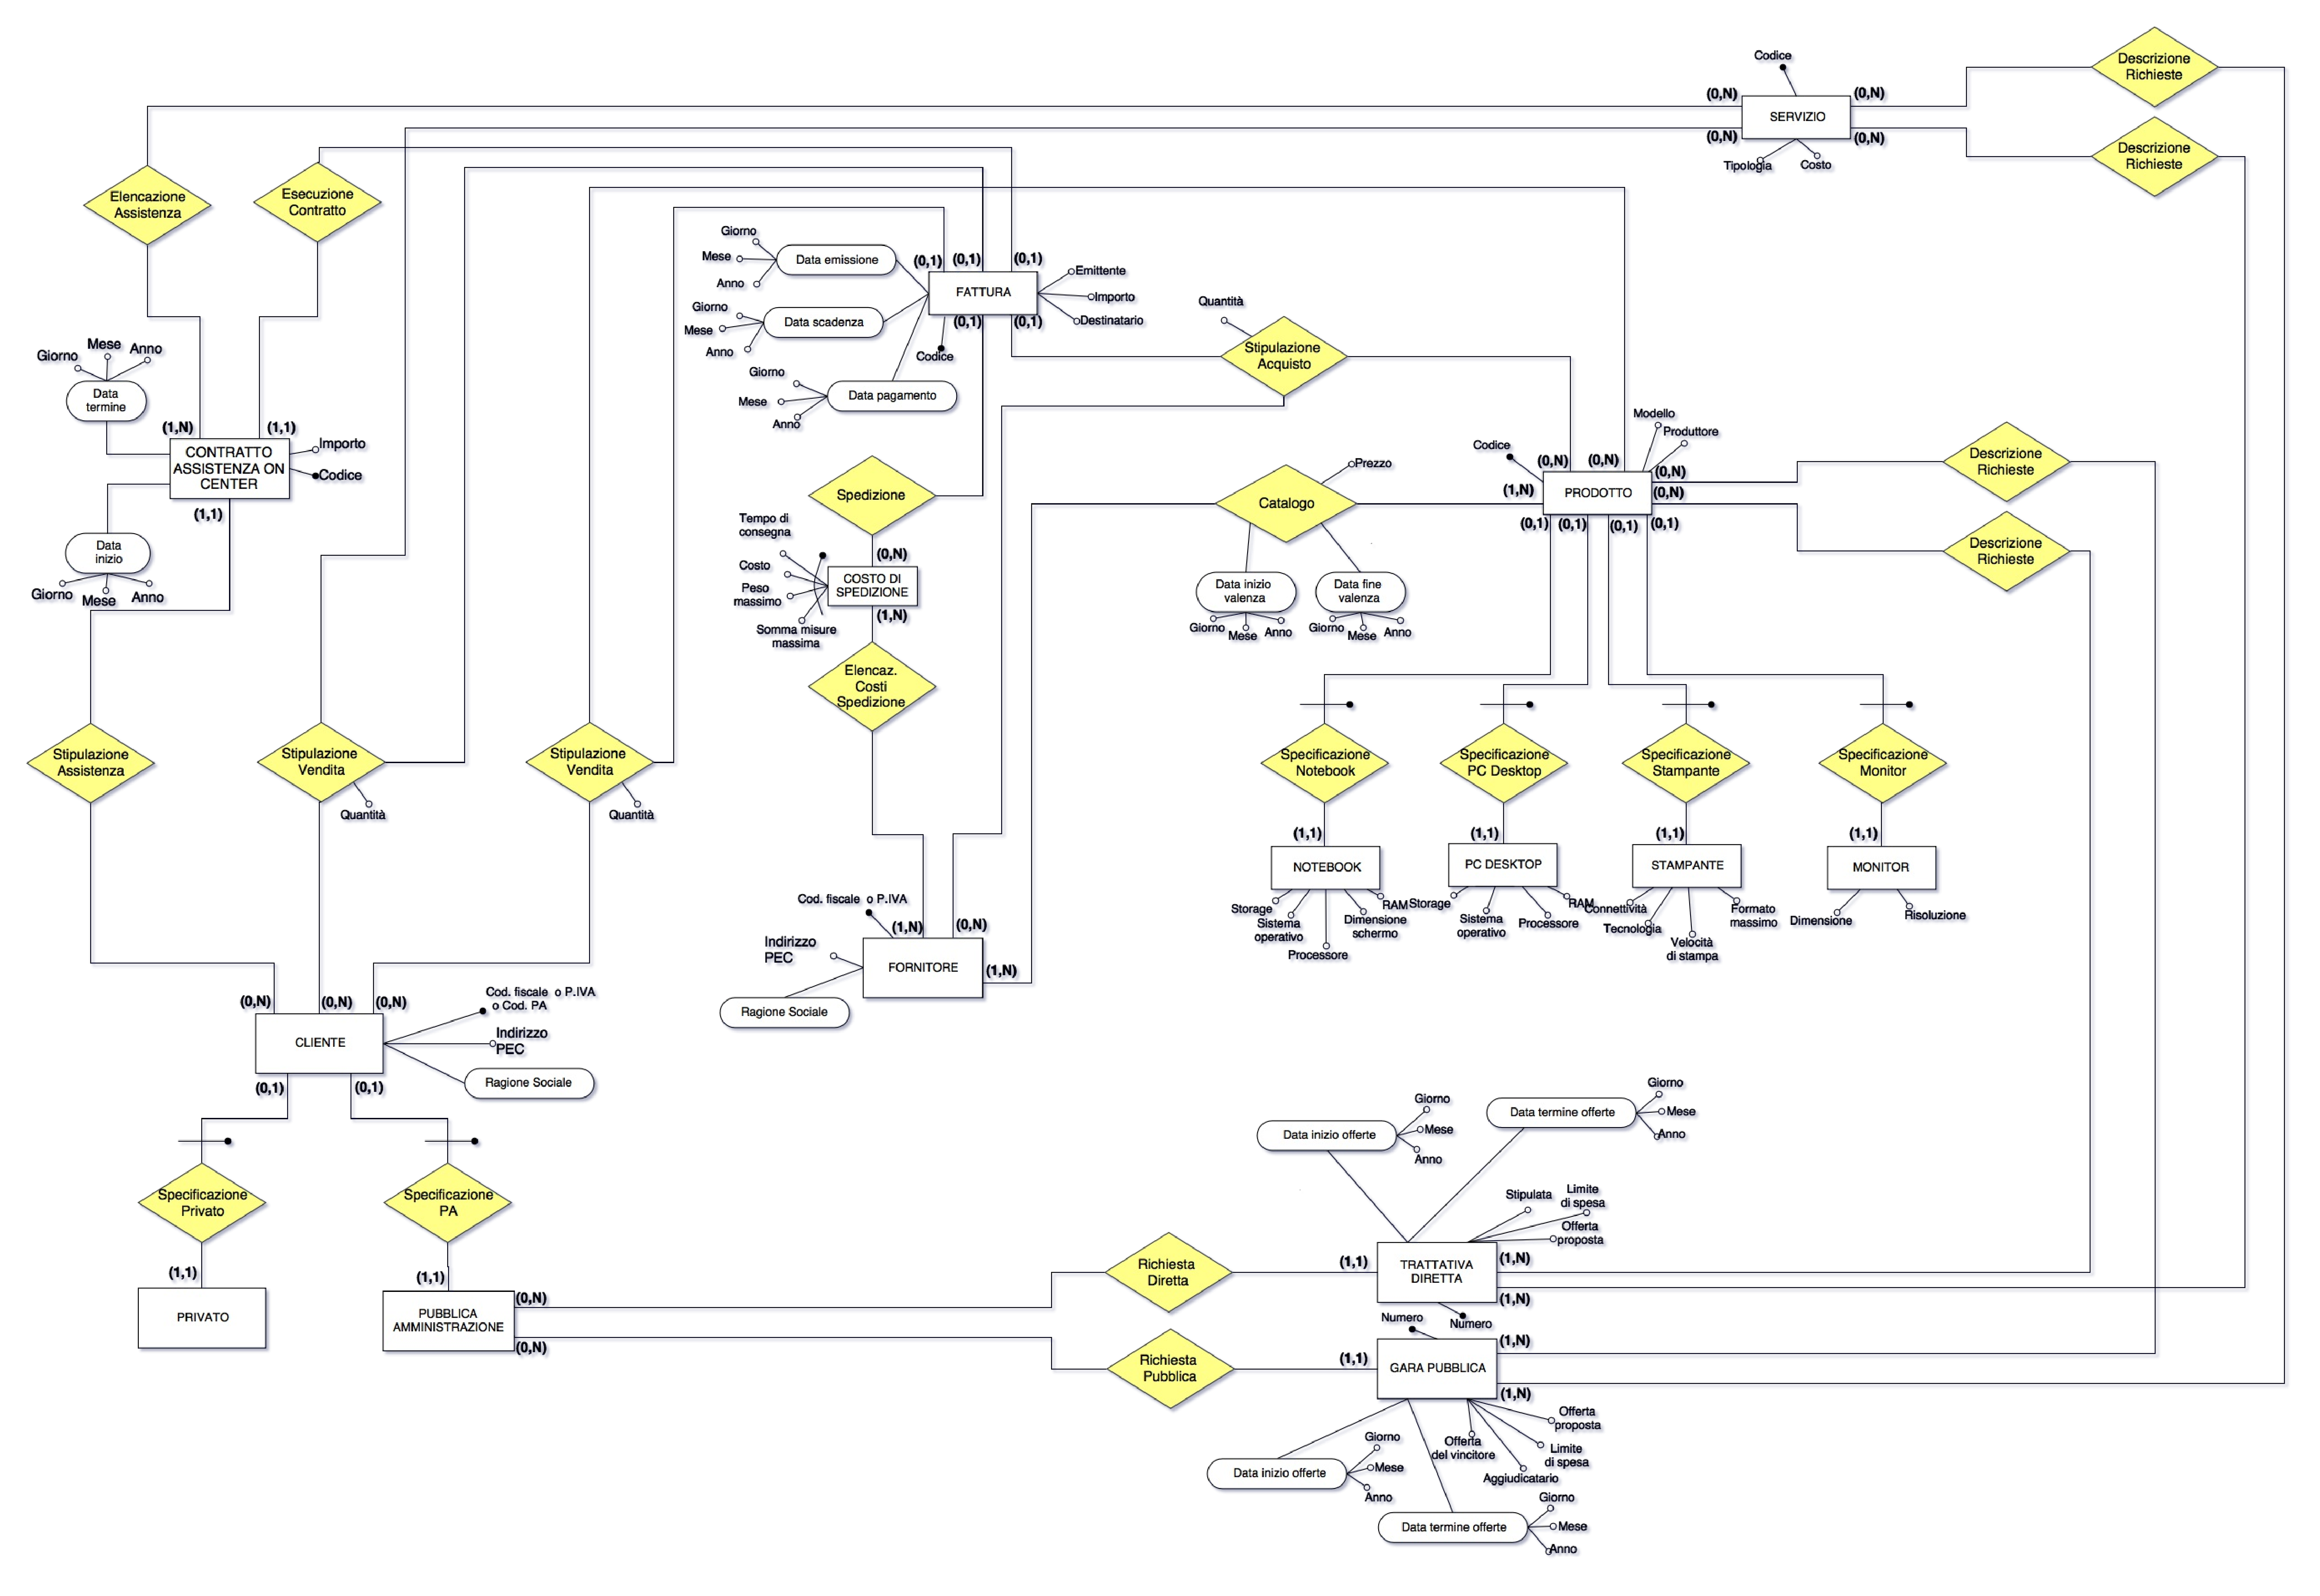
\includepdf[angle=90]{./immagini/modello_er_v3.pdf}

\end{landscape}


\newpage
\subsubsection{Eliminazione degli Attributi Multivalore}

Abbiamo individuato un solo attributo multivalore, l'attributo Telefono nelle entità Privato, Pubblica Amministrazione e Fornitore, in quanto abbiamo ritenuto che sia possibile che una di queste entità abbia più numeri di telefono associati.
\newline
Relativamente alle relazioni qui sopra citate abbiamo eseguito la ristrutturazione seguente:
\newline\newline

\noindent\makebox[\textwidth]{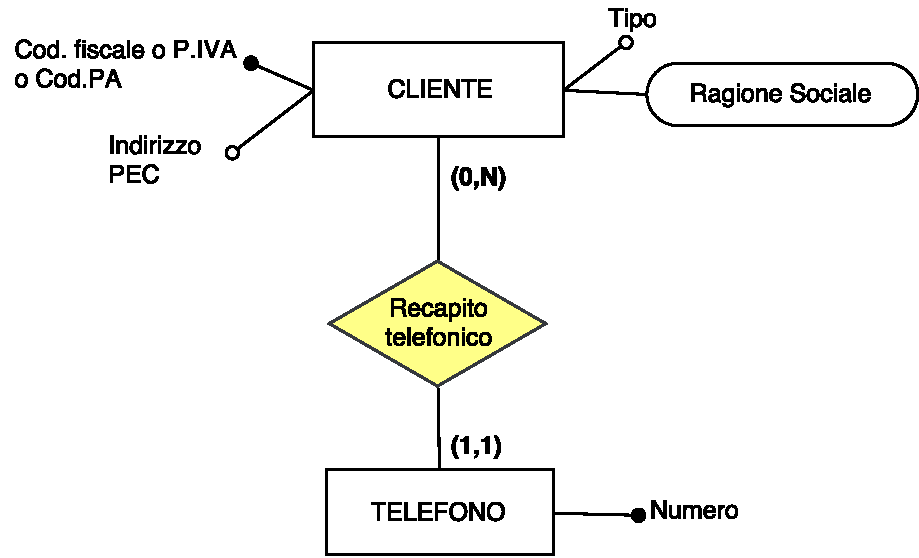
\includegraphics[width=0.7\linewidth]{./immagini/recapito_telefonico.pdf}}
\newline\newline
Tale ristrutturazione, relativa all'entità Pubblica Amministrazione, è analoga a Privato e Fornitore, perciò non vengono riportate le modifiche a tali entità.

% 		%------------------------------------------------
% 		\subsection{Elenco Identificatori Principali}
%
% 		
\begin{table}[H]
\centering
\resizebox{.65\textwidth}{!}{%
\begin{tabular}{|l|l|}
\hline
\multicolumn{1}{|c|}{\textbf{ENTIT\'{A}}} & \multicolumn{1}{c|}{\textbf{IDENTIFICATORE}} \\ \hline
Personaggio                            & Nome                                         \\ \hline
Missione                               & CodiceMiss                                   \\ \hline
Abilità                                & Nome                                         \\ \hline
Oggetto                                & Nome                                         \\ \hline
Consumo                                & CodConsumo                                   \\ \hline
Equipaggiamento                        & Nome                                         \\ \hline
Consumabili                            & Nome                                         \\ \hline
Oggetti Missione                       & Nome                                         \\ \hline
Npc Amichevole                         & Nome                                         \\ \hline
Npc Ostile                             & CodNPCOST                                    \\ \hline
Transazione                            & CodTrans                                     \\ \hline
Utente                                 & Username                                     \\ \hline
Prodotto                               & Codprodotto                                  \\ \hline
Sottoscrizione                         & CodSottoscr                                  \\ \hline
Pacchetto Oggetti                      & CodPacchOgg                                  \\ \hline
Espansione                             & CodEsp                                       \\ \hline
Carta Credito                          & numero                                       \\ \hline
\end{tabular}
}
\end{table}





\newpage


\begin{landscape} %inizia un foglio landscape

%include un file pdf che contiene lo schema 
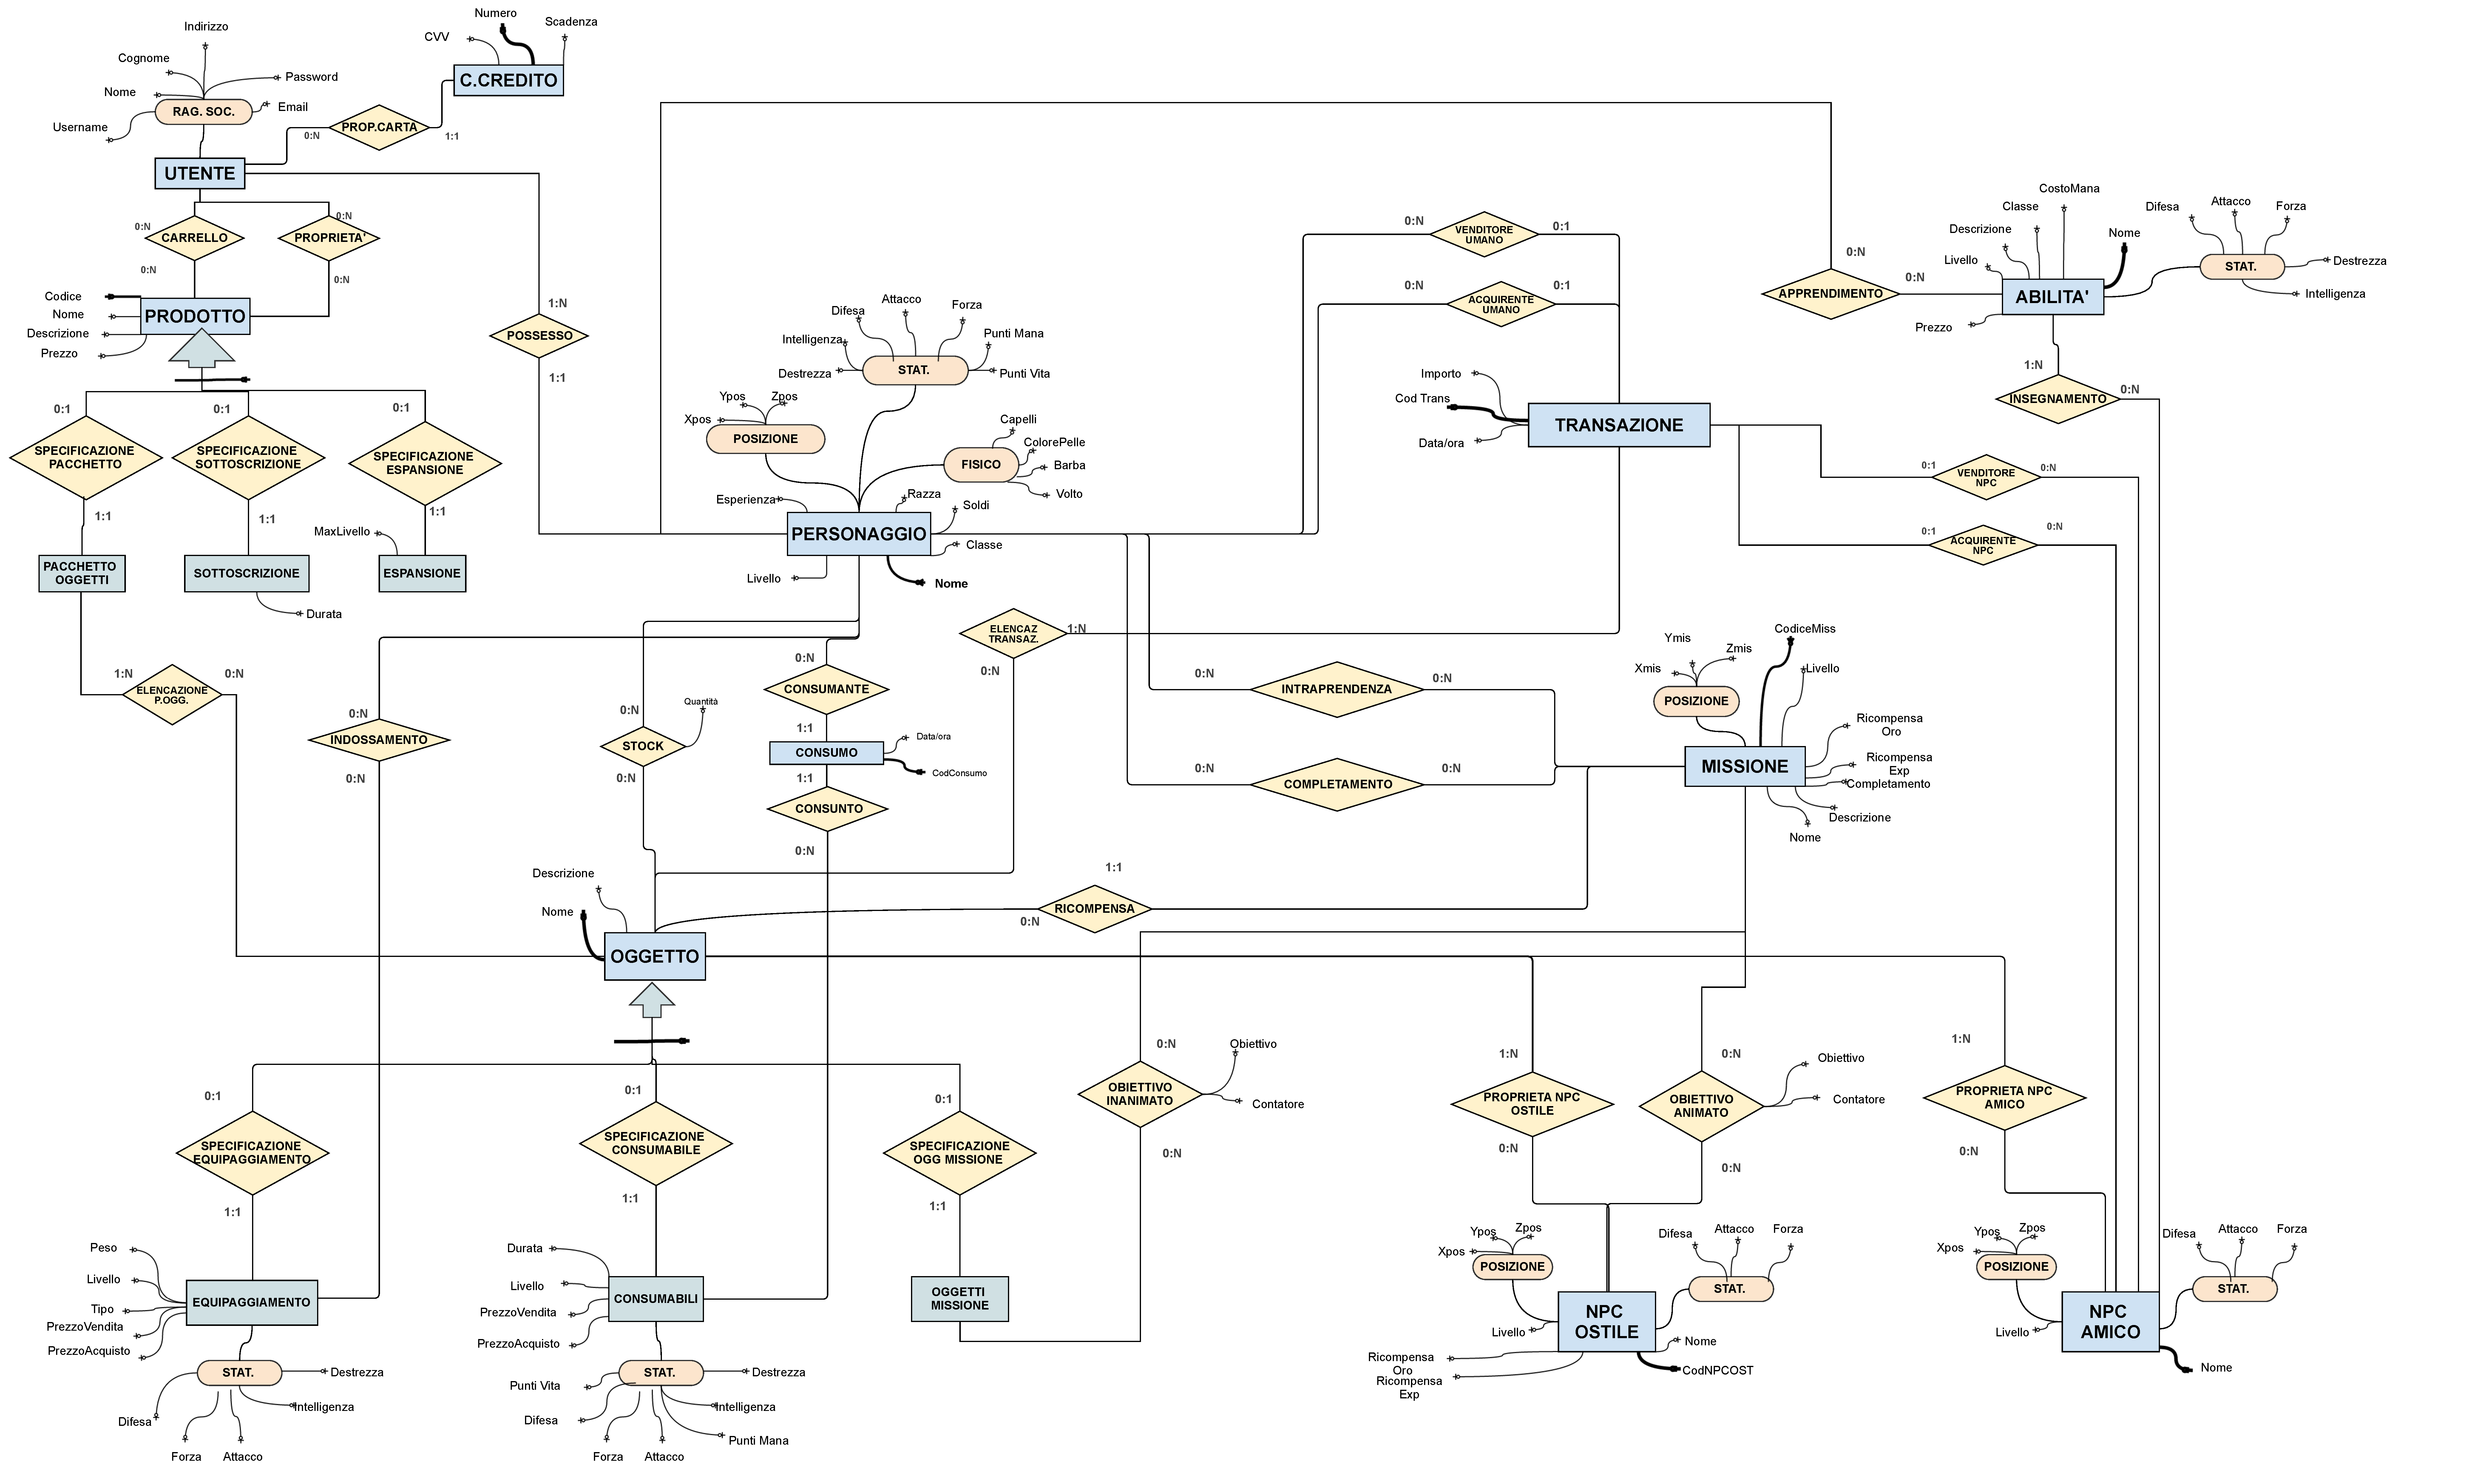
\includepdf[width=270mm, height=210mm, angle=90, keepaspectratio]{./pdf/ristrutturatocarta.pdf}

\end{landscape}
% 		%------------------------------------------------
% 		\subsection{Normalizzazione}
%
% 		
ASSOCIAZIONI:
Analizzando lo schema concettuale ristrutturato si nota che tutte le associazioni presenti sono in forma normale di 
Boyce e Codd in quanto tutte binarie.


\begin{table}[H]
\centering
\label{my-label}
\begin{tabular}{|l|l|}
\hline
\textbf{Entità}  & \textbf{Commento}                                                                                                                                             \\ \hline
Utente           & \begin{tabular}[c]{@{}l@{}}E' in terza forma normale,\\ email ? username nome cognome indirizzo\\ username è la chiave di Utente.\end{tabular}                 \\ \hline
Prodotto         & \begin{tabular}[c]{@{}l@{}}E' in forma normale di Boyce-Codd,\\ descrizione ? prezzo\\ descrizione è superchiave.\end{tabular}                                 \\ \hline
Sottoscrizione   & Non esistono dipendenze non banali fra gli attributi.                                                                                                         \\ \hline
PacchettoOggetti & Non esistono dipendenze non banali fra gli attributi.                                                                                                         \\ \hline
Espansione       & Non esistono dipendenze non banali fra gli attributi.                                                                                                         \\ \hline
Personaggio      & Non esistono dipendenze non banali fra gli attributi.                                                                                                         \\ \hline
Transazione      & Non esistono dipendenze non banali fra gli attributi.                                                                                                         \\ \hline
Consumo          & Non esistono dipendenze non banali fra gli attributi.                                                                                                         \\ \hline
Oggetto          & Non esistono dipendenze non banali fra gli attributi.                                                                                                         \\ \hline
Equipaggiamento  & Non esistono dipendenze non banali fra gli attributi.                                                                                                         \\ \hline
Consumabili      & Non esistono dipendenze non banali fra gli attributi.                                                                                                         \\ \hline
OggettiMissione  & Non esistono dipendenze non banali fra gli attributi.                                                                                                         \\ \hline
Missione         & \begin{tabular}[c]{@{}l@{}}E' in forma normale di Boyce-Codd\\ descrizione ? livello ? (tutti gli altri attributi)\\ descrizione è superchiave.\end{tabular}   \\ \hline
Abilità          & \begin{tabular}[c]{@{}l@{}}E' in forma normale di Boyce-Codd \\ descrizione ? livello ? (tutti gli altri attributi) \\ descrizione è superchiave.\end{tabular} \\ \hline
NPCAmichevole    & Non esistono dipendenze non banali fra gli attributi.                                                                                                         \\ \hline
NPCOstile        & Non esistono dipendenze non banali fra gli attributi.                                                                                                         \\ \hline
\end{tabular}
\end{table}

% 		%------------------------------------------------
% 		\subsection{Traduzione verso il Modello Relazionale}
%
% 		
\noindent\makebox[\textwidth]{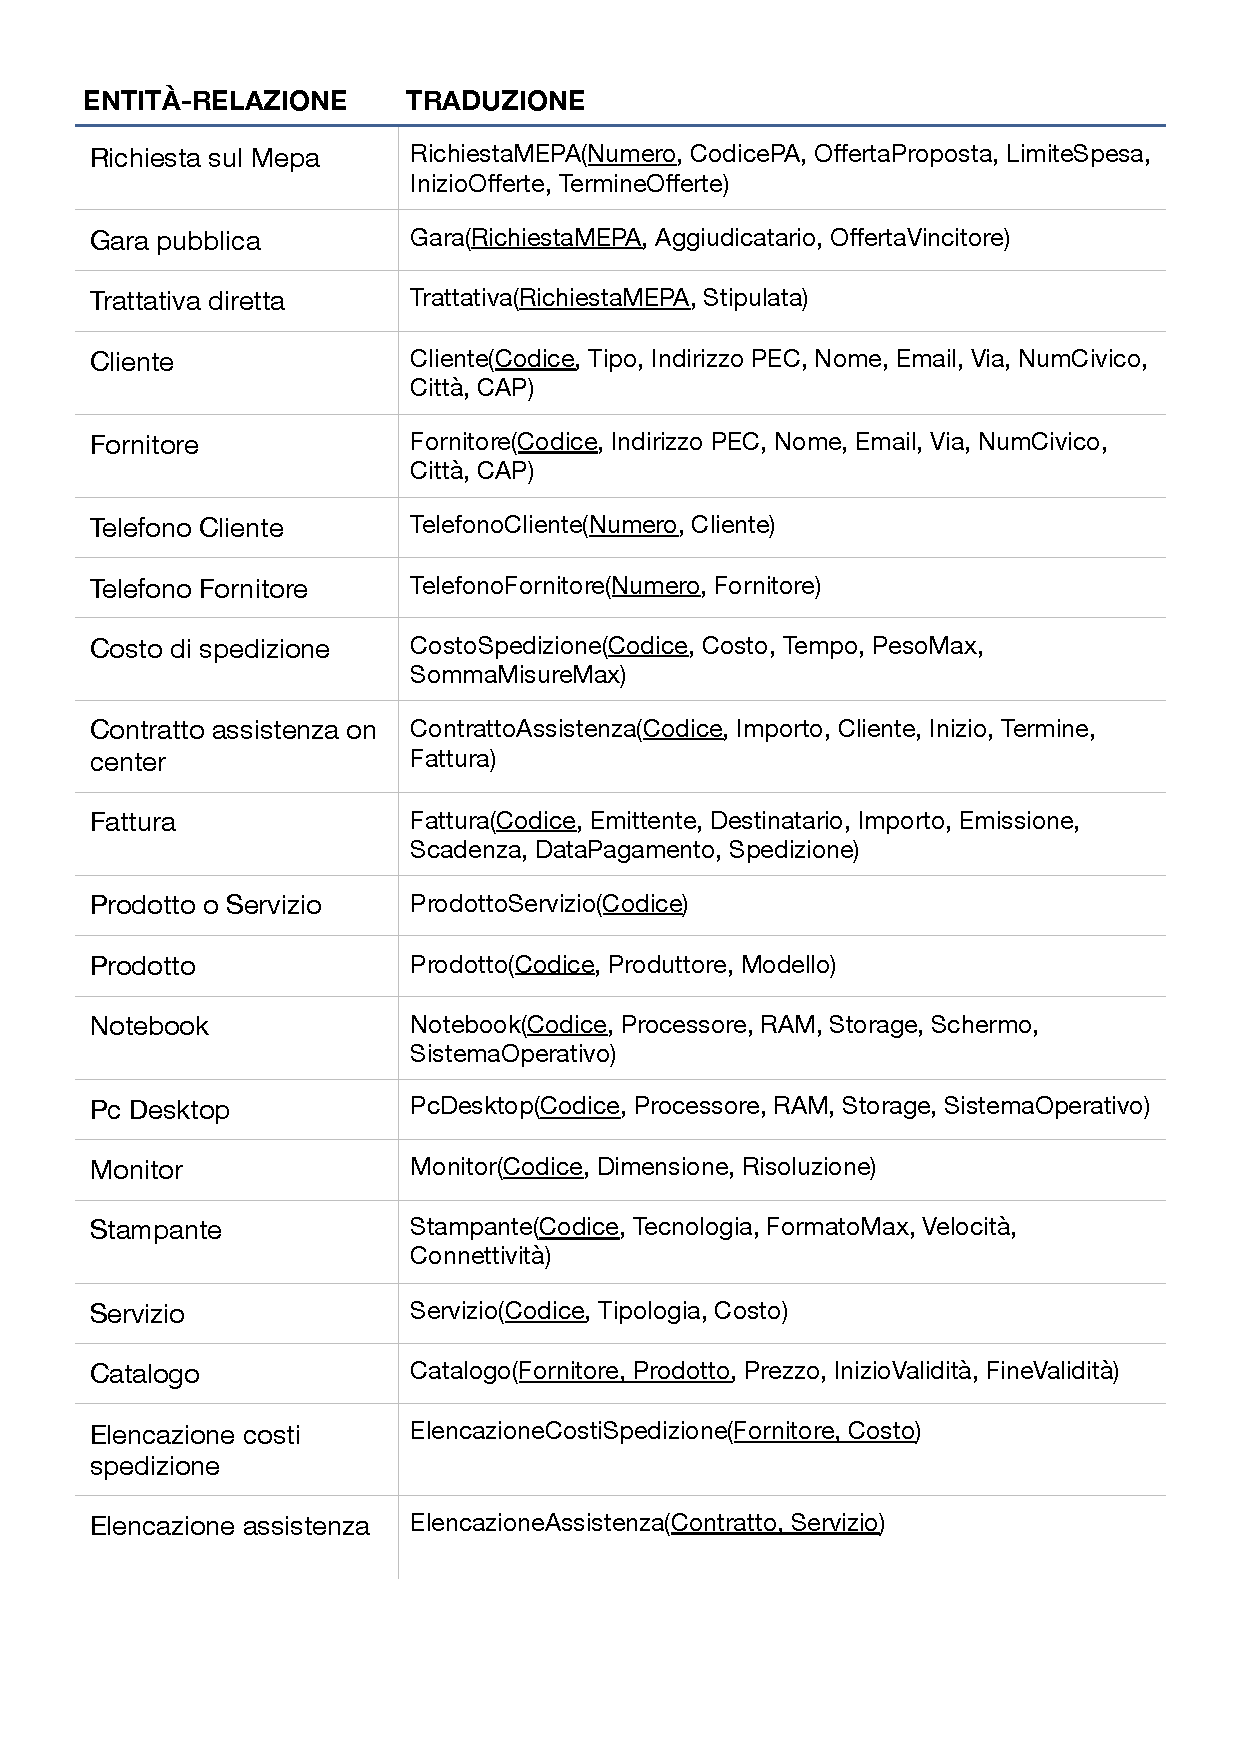
\includegraphics[width=\linewidth]{./pdf/traduzione_modello.pdf}}

%
%
% %------------------------------------------------
% 	\section{Codifica SQL e Test}
%
% 		\subsection{Definizione dello Schema e Screenshot Successivo all'Inserimento Dati}
% 		
\begin{verbatim}
create table
utente(username varchar(20) primary key, 
nome varchar(20), 
cognome varchar(20), 
indirizzo varchar(50), 
password varchar(20), 
email varchar(20)
); 

\end{verbatim}

\begin{figure}[H]
\centering
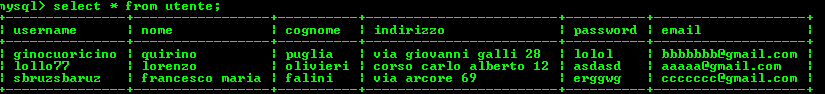
\includegraphics[width=0.7\linewidth]{immagini/1}
\caption{}
\label{fig:1}
\end{figure}

\begin{verbatim}

create table prodotto (codPro int primary key auto_increment, 
descrizione varchar(100), 
prezzo decimal(5,2),
nome varchar(20)
);FOTO2

\end{verbatim}

\begin{figure}[H]
\centering
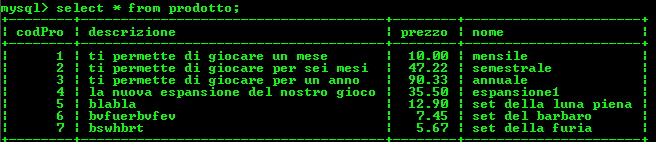
\includegraphics[width=0.7\linewidth]{immagini/2}
\caption{}
\label{fig:1}
\end{figure}

\begin{verbatim}

create table sottoscrizione( 
codSottoscr int primary key auto_increment, 
durata int, 
foreign key (codSottoscr) 
			references prodotto(codPro)
);
\end{verbatim}

\begin{figure}[H]
\centering
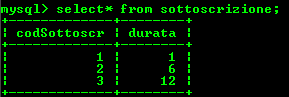
\includegraphics[width=0.7\linewidth]{immagini/3}
\caption{}
\label{fig:1}
\end{figure}

\begin{verbatim}

create table pacchettoOggetti( 
codPacchOgg int primary key auto_increment 
			references prodotto(codPro)
);
\end{verbatim}

\begin{figure}[H]
\centering
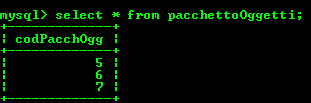
\includegraphics[width=0.7\linewidth]{immagini/4}
\caption{}
\label{fig:1}
\end{figure}

\begin{verbatim}

create table espansione( 
codEsp int primary key auto_increment 
			references prodotto(codPro), 
maxLivello int
);
\end{verbatim}

\begin{figure}[H]
\centering
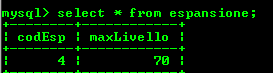
\includegraphics[width=0.7\linewidth]{immagini/5}
\caption{}
\label{fig:1}
\end{figure}

\begin{verbatim}

create table personaggio( 
nome varchar(10) primary key,
razza enum('umano','elfo','nano'), 
classe enum('guerriero','mago','arciere'), 
livello int default 1,
esperienza int default 0,
soldi int default 0, 
capelli enum('capelli1','capelli2','capelli3'), 
colorePelle enum('pelle1','pelle2','pelle3'), 
barba enum('barba1','barba2','barba3'), 
volto enum('volto1','volto2','volto3'), 
puntiVita int, 
puntiMana int, 
attacco int, 
forza int, 
destrezza int, 
intelligenza int, 
xPos int, 
yPos int, 
zPos int
nomeUt varchar(20)
			references utente(username)
);
\end{verbatim}

\begin{figure}[H]
\centering
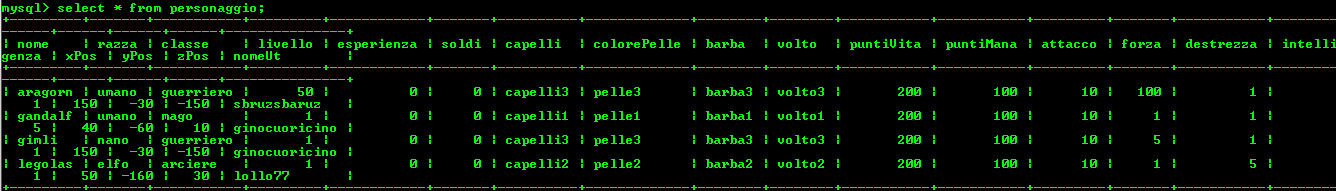
\includegraphics[width=0.7\linewidth]{immagini/6}
\caption{}
\label{fig:1}
\end{figure}

\begin{verbatim}

create table oggetto( 
nome varchar(20) primary key, 
descrizione varchar(50)
);
\end{verbatim}

\begin{figure}[H]
\centering
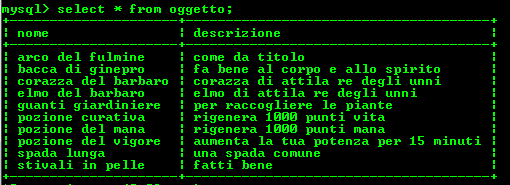
\includegraphics[width=0.7\linewidth]{immagini/7}
\caption{}
\label{fig:1}
\end{figure}

\begin{verbatim}

create table equipaggiamento(
nome varchar(20) primary key 
references oggetto(nome), 
livello int, 
tipo enum(
	'spada', 'ascia', 'mazza',
	'bastone','bacchetta', 'arco', 'balestra','stivale','guanto',
	'corazza','elmo'), 
peso enum('leggera','media','pesante'), 
attacco int, 
difesa int, 
forza int, 
destrezza int, i
ntelligenza int, 
prezzoVendita decimal(5,2), 
prezzoAcquisto decimal(5,2)
);
\end{verbatim}

\begin{figure}[H]
\centering
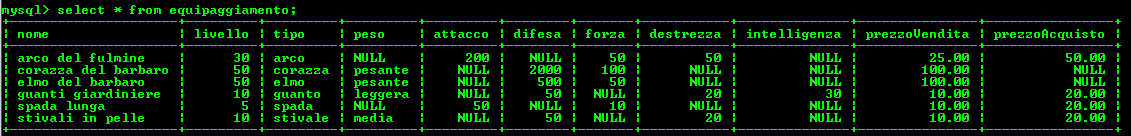
\includegraphics[width=0.7\linewidth]{immagini/8}
\caption{}
\label{fig:1}
\end{figure}

\begin{verbatim}

create table consumabili( 
nome varchar(20) primary key 
			references oggetto(nome), 
livello int, 
puntiVita int, 
puntiMana int, 
attacco int, 
difesa int, 
forza int, 
destrezza int,
intelligenza int, 
prezzoVendita decimal(5,2), 
prezzoacquisto decimal(5,2)
);
\end{verbatim}

\begin{figure}[H]
\centering
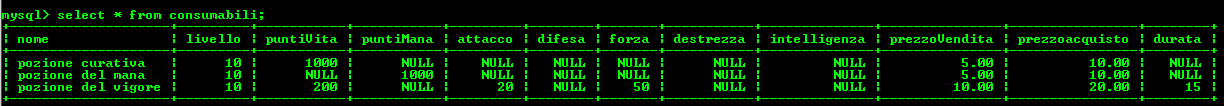
\includegraphics[width=0.7\linewidth]{immagini/9}
\caption{}
\label{fig:1}
\end{figure}

\begin{verbatim}

create table oggettiMissione( 
nome varchar(20) primary key 
			references oggetto(nome)
);
\end{verbatim}

\begin{figure}[H]
\centering
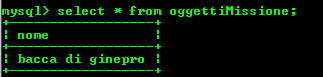
\includegraphics[width=0.7\linewidth]{immagini/10}
\caption{}
\label{fig:1}
\end{figure}

\begin{verbatim}

create table consumo( 
codConsumo int primary key auto_increment, 
dataOra time, 
consumante varchar(20) 
			references personaggio(nome), 
consunto varchar(20) 
			references consumabili(nome)
);
\end{verbatim}

\begin{figure}[H]
\centering
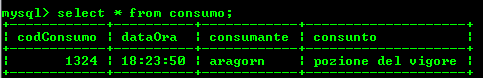
\includegraphics[width=0.7\linewidth]{immagini/11}
\caption{}
\label{fig:1}
\end{figure}

\begin{verbatim}

create table missione( 
codMiss int primary key auto_increment, 
nome varchar(50), descrizione varchar(100), 
livello int, 
completamento bool default FALSE, 
ricompensaOro int, 
ricompensaExp int, 
ricompensaOgg varchar(20) 
			references oggetti(nome), 
xMiss int, 
yMiss int, 
zMiss int
);
\end{verbatim}

\begin{figure}[H]
\centering
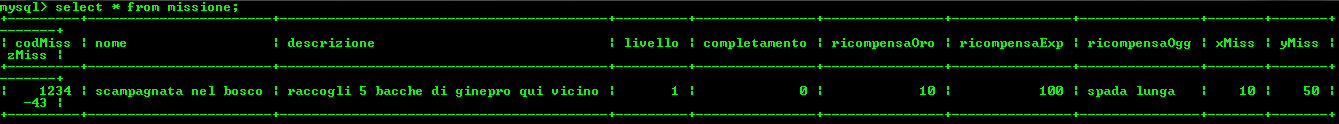
\includegraphics[width=0.7\linewidth]{immagini/12}
\caption{}
\label{fig:1}
\end{figure}

\begin{verbatim}

create table abilità( 
nome varchar(20) primary key, 
descrizione varchar(100),
classe enum('guerriero','mago','arciere'), 
livello int, 
costoMana int, 
attacco int, 
difesa int, 
forza int, 
destrezza int, 
intelligenza int, 
prezzo decimal(5,2)
);
\end{verbatim}

\begin{figure}[H]
\centering
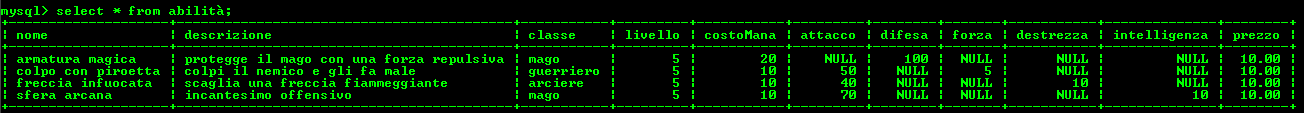
\includegraphics[width=0.7\linewidth]{immagini/13}
\caption{}
\label{fig:1}
\end{figure}

\begin{verbatim}

create table NPCAmichevole( 
nome varchar(20) primary key, 
livello int, 
puntiVita int, 
attacco int, 
difesa int, 
xPos int, 
yPos int, 
zPos int
);
\end{verbatim}

\begin{figure}[H]
\centering
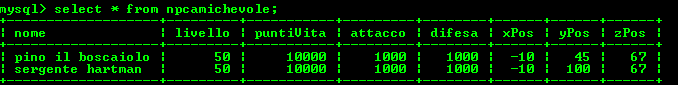
\includegraphics[width=0.7\linewidth]{immagini/14}
\caption{}
\label{fig:1}
\end{figure}

\begin{verbatim}

create table NPCOstile( 
codNPCOST int primary key auto_increment, 
nome varchar(20), 
livello int, 
puntiVita int, 
attacco int, 
difesa int, 
xPos int, 
yPos int, 
zPos int, 
ricompensaOro int, 
ricompensaExp int
);
\end{verbatim}

\begin{figure}[H]
\centering
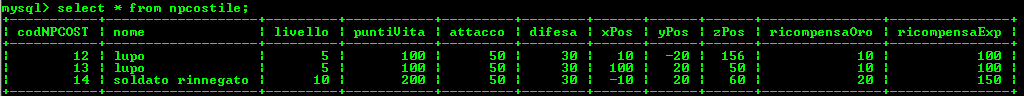
\includegraphics[width=0.7\linewidth]{immagini/15}
\caption{}
\label{fig:1}
\end{figure}

\begin{verbatim}

create table carrello(
nomeUt varchar(50) 
			references utente(username), 
codPro int 
			references prodotto(codPro), 
primary key ( nomeUt, codPro)
);
\end{verbatim}

\begin{figure}[H]
\centering
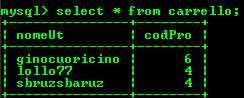
\includegraphics[width=0.7\linewidth]{immagini/16}
\caption{}
\label{fig:1}
\end{figure}

\begin{verbatim}

create table proprietà ( 
nomeUt varchar(50) 
			references utente(username), 
codPro int 
			references prodotto(codPro), 
primary key ( nomeUt, codPro)
);
\end{verbatim}

\begin{figure}[H]
\centering
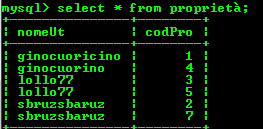
\includegraphics[width=0.7\linewidth]{immagini/17}
\caption{}
\label{fig:1}
\end{figure}

\begin{verbatim}

create table elencazionePacchettoOggetti( 
codPacchOgg int auto_increment 
			references pacchettoOggetti(codPacchOgg), 
oggetto varchar(20)
			references oggetto(nome), 
primary key (codPacchOgg,oggetto)
);
\end{verbatim}

\begin{figure}[H]
\centering
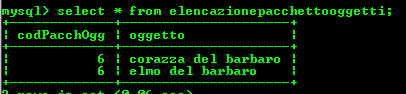
\includegraphics[width=0.7\linewidth]{immagini/18}
\caption{}
\label{fig:1}
\end{figure}

\begin{verbatim}

create table intraprendenza(
personaggio varchar(30) 
			references personaggio(nome), 
missione int  
			references missione(codMiss), 
primary key (personaggio, missione)
);
\end{verbatim}

\begin{figure}[H]
\centering
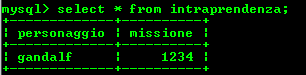
\includegraphics[width=0.7\linewidth]{immagini/19}
\caption{}
\label{fig:1}
\end{figure}

\begin{verbatim}

create table completamento(  
personaggio varchar(30)
			references personaggio(nome), 
missione int  
			references missione(codMiss), 
primary key (personaggio, missione)
);
\end{verbatim}

\begin{figure}[H]
\centering
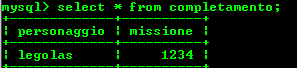
\includegraphics[width=0.7\linewidth]{immagini/20}
\caption{}
\label{fig:1}
\end{figure}

\begin{verbatim}

create table obiettivoAnimato( 
missione int 
			references missione(codMiss), 
nemico int 
			references NPCOstile (codNPCOst), 
primary key (missione,nemico), 
obiettivo int, 
contatore int
);Senza Foto

create table obiettivoInanimato( 
missione int 
			references missione(codMiss), 
oggMiss varchar(20) 
			references oggettiMissione(nome), 
primary key (missione,oggMiss), 
obiettivo int, 
contatore int
);
\end{verbatim}

\begin{figure}[H]
\centering
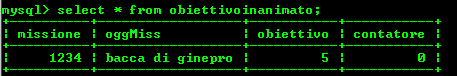
\includegraphics[width=0.7\linewidth]{immagini/21}
\caption{}
\label{fig:1}
\end{figure}

\begin{verbatim}

create table apprendimento(
personaggio varchar(20) 
		references personaggio(nome), 
abilità varchar(20) 
		references abilità(nome), 
primary key(personaggio,abilità)
);

\end{verbatim}

\begin{figure}[H]
\centering
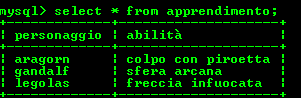
\includegraphics[width=0.7\linewidth]{immagini/22}
\caption{}
\label{fig:1}
\end{figure}

\begin{verbatim}

create table insegnamento(
maestro varchar(20) 
			references NPCAmichevole(nome), 
abilità varchar(20) 
			references abilità(nome), 
primary key(maestro,abilità)
);
\end{verbatim}

\begin{figure}[H]
\centering
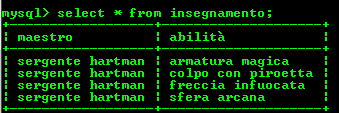
\includegraphics[width=0.7\linewidth]{immagini/23}
\caption{}
\label{fig:1}
\end{figure}

\begin{verbatim}

create table proprietàNPCAmichevole( 
venditore varchar(20) 
			references NPCAmichevole (nome), 
oggetto varchar(20) 
			references oggetto(nome), 
primary key (venditore,oggetto)
);
\end{verbatim}

\begin{figure}[H]
\centering
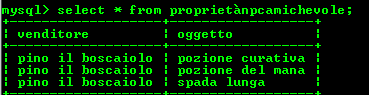
\includegraphics[width=0.7\linewidth]{immagini/24}
\caption{}
\label{fig:1}
\end{figure}

\begin{verbatim}

create table proprietàNPCOstile( 
nemico int 
			references NPCOstile (codNPCOst), 
oggetto varchar(20) 
			references oggetto(nome), 
primary key (nemico,oggetto)
);
\end{verbatim}

\begin{figure}[H]
\centering
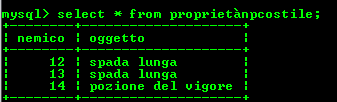
\includegraphics[width=0.7\linewidth]{immagini/25}
\caption{}
\label{fig:1}
\end{figure}

\begin{verbatim}

create table stock( 
personaggio varchar(20) 
			references personaggio(nome), 
oggetto varchar(20)
			references oggetto(nome),
primary key (personaggio,oggetto)
);
\end{verbatim}

\begin{figure}[H]
\centering
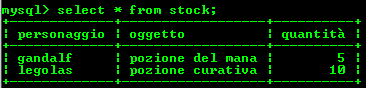
\includegraphics[width=0.7\linewidth]{immagini/26}
\caption{}
\label{fig:1}
\end{figure}

\begin{verbatim}

create table indossamento( 
personaggio varchar(20) 
			references personaggio(nome), 
oggEquip varchar(20) 
			references equipaggiamento(nome),
primary key (personaggio,oggEquip)
);FOTO29
\end{verbatim}

\begin{figure}[H]
\centering
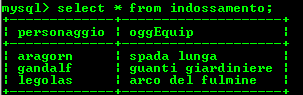
\includegraphics[width=0.7\linewidth]{immagini/27}
\caption{}
\label{fig:1}
\end{figure}

\begin{verbatim}

create table transazione(
codTrans int auto_increment primary key,
dataOra time, 
importo decimal(5,2), 
compratoreReale varchar(20) 
			references personaggio(nome), 

venditoreReale varchar(20) 
			references personaggio(nome), 
compratorePC varchar(20) 
			references NPCAmichevole(nome), 
venditorePC varchar(20) 
			references NPCAmichevole(nome)
);

\end{verbatim}

\begin{figure}[H]
\centering
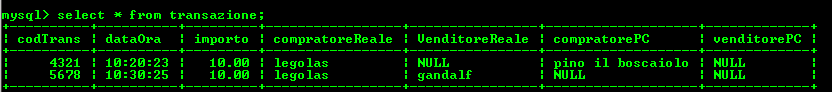
\includegraphics[width=0.7\linewidth]{immagini/28}
\caption{}
\label{fig:1}
\end{figure}

\begin{verbatim}
create table ElencazioneTransazione( 
transazione int 
			references transazione(codTrans), 
oggetto varchar(20)
			references oggetto(nome), 
primary key(transazione,oggetto)
);
\end{verbatim}

\begin{figure}[H]
\centering
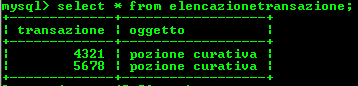
\includegraphics[width=0.7\linewidth]{immagini/29}
\caption{}
\label{fig:1}
\end{figure}

\begin{verbatim}

create table cartaCredito( 
numero int primary key, 
cvv int, 
scadenza date, 
nomeUt varchar(20) 
		references utente(username)
);
\end{verbatim}

\begin{figure}[H]
\centering
\includegraphics[width=0.7\linewidth]{immagini/30}
\caption{}
\label{fig:1}
\end{figure}

\begin{verbatim}

\end{verbatim}

%
% 		%------------------------------------------------
%
% 		\subsection{Codifica delle Operazioni}
%
% 		\vspace{1cm}

\noindent\textit{Inserimento nuovo cliente (in media 10 volte al mese)}
\begin{verbatim}
insert into Cliente(Codice, Tipo, IndirizzoPEC, Nome, Email, Via,
  NumCivico, Citta, CAP)
  values(...);
insert into TelefonoCliente(Numero, Cliente)
  values(...);
\end{verbatim}
\vspace{1cm}

\noindent\textit{Inserimento nuova gara pubblica (in media una volta al giorno)}
\begin{verbatim}
insert into Cliente(Codice, Tipo, IndirizzoPEC, Nome, Email, Via,
  NumCivico, Citta, CAP)
  values(...);
insert into TelefonoCliente(Numero, Cliente)
  values(...);
insert into RichiestaMEPA(Numero, CodicePA, OffertaProposta, LimiteSpesa,
  InizioOfferte, TermineOfferte)
  values(...);
insert into Gara(RichiestaMEPA, Aggiudicatario, OffertaVincitore)
  values(...);
\end{verbatim}
\vspace{1cm}

\noindent\textit{Inserimento nuova trattativa diretta (in media una volta a settimana)}
\begin{verbatim}
insert into Cliente(Codice, Tipo, IndirizzoPEC, Nome, Email, Via,
  NumCivico, Citta, CAP)
  values(...);
insert into TelefonoCliente(Numero, Cliente)
  values(...);
insert into RichiestaMEPA(Numero, CodicePA, OffertaProposta, LimiteSpesa,
  InizioOfferte, TermineOfferte)
  values(...);
insert into Trattativa(RichiestaMEPA, Stipulata)
  values(...);
\end{verbatim}
\vspace{1cm}

\noindent\textit{Inserimento nuovo prodotto (due volte al mese)}
\begin{verbatim}
/* notebook */
insert into ProdottoServizio(Codice) values (...);
insert into Prodotto(Codice, Produttore, Modello)
  values(...);
insert into Notebook(Codice, Processore, RAM, Storage, Schermo,
  SistemaOperativo)
  values(...);
\end{verbatim}
\vspace{1cm}

\noindent\textit{Inserimento nuova fattura (in media tre volte al giorno)}
\begin{verbatim}
insert into Fattura(Codice, Emittente, Destinatario, Importo, Emissione,
  Scadenza, DataPagamento, Spedizione)
  values(null, ...);

/* acquisto prodotto */
insert into Fattura(Codice, Emittente, Destinatario, Importo, Emissione,
  Scadenza, DataPagamento, Spedizione)
  values(null, <codice_fornitore>, 'Rimini Service', ...);
insert into Acquisto(Fattura, Prodotto, Quantita)
  values((select max(Codice) from Fattura), ...);
update Fattura
  set Importo = (
    select sum(Quantita*Prezzo)
      from (select min(Prezzo) as Prezzo, Fornitore
        from Catalogo
        where Prodotto = <codice_prodotto> and InizioValidita < NOW()
        and FineValidita > NOW()
        group by Fornitore
      ) as PrezzoVendita, Acquisto
      where Acquisto.Fattura = (select max(Fattura) from Acquisto)
      and Acquisto.Prodotto = <codice_prodotto>
  ),
  Spedizione = (
    select Codice
      from CostoSpedizione, ElencazioneCostiSpedizione
      where (select Peso
          from Prodotto
          where Codice = <codice_prodotto>) <= PesoMax
      and (select
        (select SUBSTRING_INDEX(Dimensioni, 'x', 1) from Prodotto
        where Codice = <codice_prodotto>) +
        (select SUBSTRING_INDEX(SUBSTRING_INDEX(Dimensioni, 'x', 2), 'x', 1)
        from Prodotto where Codice = <codice_prodotto>) +
        (select SUBSTRING_INDEX(Dimensioni, 'x', -1) from Prodotto
        where Codice = <codice_prodotto>)
        ) <= SommaMisureMax
      and ElencazioneCostiSpedizione.Fornitore = Fattura.Emittente
      order by CostoSpedizione.Costo limit 1
  )
  order by Codice DESC limit 1;

/* vendita prodotto */
insert into Fattura(Codice, Emittente, Destinatario, Importo, Emissione,
  Scadenza, DataPagamento, Spedizione)
  values(null, ...);
insert into Vendita(Fattura, ProdottoServizio, Quantita)
  values((select max(Codice) from Fattura), ...)
update Fattura
  set Importo = (
    select sum(Quantita*Prezzo*1.1) + (select Costo
        from CostoSpedizione
        where (select Peso
            from Prodotto
            where Codice = <codice_prodotto>) <= PesoMax
        and (select
          (select SUBSTRING_INDEX(Dimensioni, 'x', 1) from Prodotto
          where Codice = <codice_prodotto>) +
          (select SUBSTRING_INDEX(SUBSTRING_INDEX(Dimensioni, 'x', 2), 'x', 1)
          from Prodotto where Codice = <codice_prodotto>) +
          (select SUBSTRING_INDEX(Dimensioni, 'x', -1) from Prodotto
          where Codice = <codice_prodotto>)
          ) <= SommaMisureMax
        order by Costo limit 1)
      from (select min(Prezzo) as Prezzo, Fornitore
        from Catalogo
        where Prodotto = <codice_prodotto> and InizioValidita < NOW()
        and FineValidita > NOW()
        group by Fornitore
      ) as PrezzoVendita, Vendita
      where Vendita.Fattura = (select max(Fattura) from Vendita)
      and Vendita.ProdottoServizio = <codice_prodotto>
  )
  order by Codice DESC limit 1;
\end{verbatim}
\vspace{1cm}

\noindent\textit{Stipulazione nuovo contratto di assistenza on center (una volta al mese)}
\begin{verbatim}
insert into Fattura(Codice, Emittente, Destinatario, Importo, Emissione,
  Scadenza, DataPagamento, Spedizione)
  values(null, 'Rimini Service', <codice_cliente>, <importo_contratto>,
  NOW(), adddate(NOW(), 30), null, null);
insert into ContrattoAssistenza(Codice, Importo, Cliente, Inizio, Termine,
  Fattura)
  values(null, ..., (select max(Codice) from Fattura));
insert into ElencazioneAssistenza(Contratto, Servizio)
  values ((select max(Codice) from ContrattoAssistenza), <codice_servizio>);
\end{verbatim}
\vspace{1cm}

\noindent\textit{Aggiornamento di una gara pubblica in seguito alla sua chiusura (in media una volta al giorno)}
\begin{verbatim}
update Gara set Aggiudicatario = <vincitore>, OffertaVincitore = <offerta>
  where RichiestaMEPA = <codice_gara>;
\end{verbatim}
\vspace{1cm}

\noindent\textit{Aggiornamento di un catalogo (dieci volte al mese)}
\begin{verbatim}
update Catalogo
  set Prezzo = <nuovo_prezzo>, InizioValidita = <nuovo_inizio>,
  FineValidita = <nuovo_termine>
  where Fornitore = <fornitore> and Prodotto = <prodotto>;
\end{verbatim}
\vspace{1cm}

\noindent\textit{Cancellazione di un prodotto (quattro volte all'anno)}
\begin{verbatim}
delete from ProdottoServizio
  where Codice = <codice_prodotto_servizio>;
\end{verbatim}
\vspace{1cm}

\noindent\textit{Cancellazione di un fornitore (una volta all'anno)}
\begin{verbatim}
delete from Fornitore
  where Codice = <codice_fornitore>;
\end{verbatim}
\vspace{1cm}

\noindent
Qui dobbiamo sottolineare come le operazioni di cancellazione riportate, come quelle non riportate in quanto simili, non siano del tutto corrette. Infatti in tal caso la cancellazione di un Fornitore ad esempio può suscitare problematiche se il Fornitore cancellato faceva parte di altri record, come foreign key, o semplicemente come dato di rilevanza per caratterizzare la riga. In questo caso si è preferito trascurare il problema, in quanto la sua gestione porta a pensare la gestione delle tabelle in maniera diversa. Infatti il modo più corretto per ovviare a questa problematica, come è usato in ambito aziendale, è quello di inserire un campo booleano "deleted" che serve a tenere traccia di quando una riga sarebbe stata cancellata. Nel momento della cancellazione il campo viene messo a true, e in questo modo non si causano ripercussioni a catena sulla base di dati. Per tenere conto di questo campo tutte le consultazioni effettuate sul database devono avere la condizione che il campo deleted sia false, quindi il record è valido e dev'essere considerato. Per semplicità in questo progetto si è trascurato tutto questo meccanismo, che andrebbe risolto come descritto.
\vspace{1cm}

\noindent\textit{Aggiornamento di un catalogo (dieci volte al mese)}
\begin{verbatim}
update Catalogo
  set Prezzo = <nuovo_prezzo>, InizioValidita = <nuovo_inizio>,
  FineValidita = <nuovo_termine>
  where Fornitore = <fornitore> and Prodotto = <prodotto>;
\end{verbatim}
\vspace{1cm}

\noindent\textit{Consultazione dati dei clienti (in media 10 volte al giorno)}
\begin{verbatim}
select * from Cliente where Codice = <codice_cliente>;
\end{verbatim}
\vspace{1cm}

\noindent\textit{Consultazione contratti di assistenza on center (in media due volte a settimana)}
\begin{verbatim}
select (select Nome from Cliente where Codice=Cliente) as Cliente,
  ContrattoAssistenza.Importo, Inizio, Termine, DataPagamento
  from ContrattoAssistenza, Fattura
  where ContrattoAssistenza.Codice = <codice_contratto>
  and Fattura.Codice = ContrattoAssistenza.Fattura;
\end{verbatim}
\vspace{1cm}

\noindent\textit{Consultazione contratti di assistenza on center in un determinato periodo (due volte al mese)}
\begin{verbatim}
select ContrattoAssistenza.Codice as Contratto, (select Nome from Cliente
  where Codice=Cliente) as Cliente, ContrattoAssistenza.Importo, Inizio,
  Termine, DataPagamento
  from ContrattoAssistenza, Fattura
  where Inizio >= <data_inizio> and Termine <= <data_termine>
  and Fattura.Codice = ContrattoAssistenza.Fattura;

\end{verbatim}
\vspace{0.5cm}

\noindent\makebox[\textwidth]{\includegraphics[width=\linewidth]{./immagini/op1}}
\newline\newline

\noindent\textit{Consultazione dati di una gara pubblica (in media cinque volte al giorno)}
\begin{verbatim}
select * from Gara where RichiestaMEPA = <numero_richiestamepa>;
\end{verbatim}
\vspace{1cm}

\noindent\textit{Consultazione dati di una trattativa diretta (in media due volte al giorno)}
\begin{verbatim}
select * from Trattativa where RichiestaMEPA = <numero_richiestamepa>;
\end{verbatim}
\vspace{1cm}

\noindent\textit{Consultazione caratteristiche di un prodotto (cinque volte al giorno)}
\begin{verbatim}
/* monitor per codice */
select Prodotto.Codice, Produttore, Modello, Dimensione, Risoluzione
  from Prodotto, Monitor
  where Prodotto.Codice = Monitor.Codice
  and Monitor.Codice = <codice_monitor>;

/* notebook per codice */
select Prodotto.Codice, Produttore, Modello, Processore, RAM, Storage,
  Schermo, SistemaOperativo
  from Prodotto, Notebook
  where Prodotto.Codice = Notebook.Codice
  and Notebook.Codice = <codice_notebook>;

/* pcdesktop per codice */
select Prodotto.Codice, Produttore, Modello, Processore, RAM, Storage,
  SistemaOperativo
  from Prodotto, PCDesktop
  where Prodotto.Codice = PCDesktop.Codice
  and PCDesktop.Codice = <codice_pcdesktop>;
\end{verbatim}
\vspace{0.5cm}

\noindent\makebox[\textwidth]{\includegraphics[width=\linewidth]{./immagini/op2}}
\newline\newline

\noindent\textit{Consultazione prezzo di un prodotto (dieci volte al giorno)}
\begin{verbatim}
select min(Prezzo) as Prezzo, Fornitore
  from Catalogo
  where Prodotto = <codice_prodotto> and InizioValidita < NOW()
  and FineValidita > NOW()
  group by Fornitore;
\end{verbatim}
\vspace{0.5cm}

\noindent\makebox[\textwidth]{\includegraphics[width=\linewidth]{./immagini/op3}}
\newline\newline

\noindent\textit{Consultazione di una fattura (una volta al giorno)}
\begin{verbatim}
select * from Fattura where Codice = <codice_fattura>;
\end{verbatim}
\vspace{1cm}

\noindent\textit{Statistica delle gare pubbliche vinte e perse in un determinato periodo (una volta al mese)}
\begin{verbatim}
select Gara.RichiestaMEPA, Aggiudicatario, OffertaVincitore, LimiteSpesa
  from Gara, RichiestaMEPA
  where TermineOfferte >= <inizio_periodo>
  and TermineOfferte <= <fine_periodo>
  and Gara.RichiestaMEPA = RichiestaMEPA.Numero
  order by Aggiudicatario = 'Rimini Service' desc;
\end{verbatim}
\vspace{0.5cm}

\noindent\makebox[\textwidth]{\includegraphics[width=\linewidth]{./immagini/op4}}
\newline\newline

\noindent\textit{Statistica delle trattative dirette stipulate (una volta al mese)}
\begin{verbatim}
select * from Trattativa order by Stipulata = true desc;
\end{verbatim}
\vspace{0.5cm}

\noindent\makebox[\textwidth]{\includegraphics[width=\linewidth]{./immagini/op5}}
\newline\newline

\noindent\textit{Statistica dei prodotti più venduti (una volta al mese)}
\begin{verbatim}
select Codice, Quantita, Produttore, Modello
  from Vendita, Prodotto
  where Vendita.ProdottoServizio = Codice
  order by Quantita desc;
\end{verbatim}
\vspace{0.5cm}

\noindent\makebox[\textwidth]{\includegraphics[width=0.7\linewidth]{./immagini/op6}}
\newline\newline

\noindent\textit{Statistica dei servizi più erogati (una volta al mese)}
\begin{verbatim}
select Servizio, count(*) as Frequenza
  from ElencazioneAssistenza
  group by Servizio
  order by Frequenza desc;
\end{verbatim}
\vspace{0.5cm}

\noindent\makebox[\textwidth]{\includegraphics[width=0.6\linewidth]{./immagini/op7}}
\newline\newline

\noindent\textit{Verifica del pagamento delle fatture da parte dei clienti (due volte a settimana)}
\begin{verbatim}
select Codice, (select Nome from Cliente where Codice=Destinatario)
  as Nome, Emissione, Scadenza
  from Fattura
  where Emittente='Rimini Service' and NOW() >= Emissione
  and DataPagamento IS NULL
  order by Emissione;
\end{verbatim}
\vspace{0.5cm}

\noindent\makebox[\textwidth]{\includegraphics[width=\linewidth]{./immagini/op8}}
\newline\newline

\noindent\textit{Verifica di scadenza imminente del pagamento delle fatture da parte dei clienti (tre volte al mese)}
\begin{verbatim}
select Codice, (select Nome from Cliente where Codice=Destinatario)
  as Nome, Emissione, Scadenza
  from Fattura
  where Emittente='Rimini Service' and NOW() >= Emissione
  and DataPagamento IS NULL and DATEDIFF(Scadenza, NOW()) < 3
  order by Emissione;
\end{verbatim}
\vspace{0.5cm}

\noindent\makebox[\textwidth]{\includegraphics[width=\linewidth]{./immagini/op9}}
\newline\newline

\noindent\textit{Verifica del pagamento delle fatture da parte dell'azienda (due volte a settimana)}
\begin{verbatim}
select Codice, (select Nome from Fornitore where Codice=Emittente)
  as Fornitore, Emissione, Scadenza
  from Fattura
  where Destinatario='Rimini Service'
  and NOW() >= Emissione and DataPagamento IS NULL
  order by Emissione;
\end{verbatim}
\vspace{0.5cm}

\noindent\makebox[\textwidth]{\includegraphics[width=\linewidth]{./immagini/op10}}
\newline\newline

\noindent\textit{Verifica di scadenza imminente del pagamento delle fatture da parte dell'azienda (tre volte al mese)}
\begin{verbatim}
select Codice, (select Nome from Fornitore where Codice=Emittente)
  as Fornitore, Emissione, Scadenza
  from Fattura
  where Destinatario='Rimini Service'
  and NOW() >= Emissione and DataPagamento IS NULL
  and DATEDIFF(Scadenza, NOW()) < 3
  order by Emissione;
\end{verbatim}
\vspace{0.5cm}

\noindent\makebox[\textwidth]{\includegraphics[width=\linewidth]{./immagini/op11}}
\newline\newline

\noindent\textit{Calcolo del guadagno netto ad una certa data (una volta al mese)}
\begin{verbatim}
select ((select sum(Importo) from Fattura where Emittente = 'Rimini Service')
  - (select sum(Importo) from Fattura where Emittente != 'Rimini Service'))
  as Guadagno;
\end{verbatim}
\vspace{0.5cm}

\noindent\makebox[\textwidth]{\includegraphics[width=\linewidth]{./immagini/op12}}
\newline\newline

\noindent\textit{Calcolo del volume di vendite in un determinato periodo (una volta al mese)}
\begin{verbatim}
select sum(Importo) as Volume_vendite
  from Fattura
  where Emittente = 'Rimini Service' and Emissione >= <inizio_periodo>
  and Emissione <= <fine_periodo>;
\end{verbatim}
\vspace{0.5cm}

\noindent\makebox[\textwidth]{\includegraphics[width=\linewidth]{./immagini/op13}}
\newline\newline

\noindent\textit{Calcolo dei costi di spedizione di un'acquisto (tre volte al giorno)}
\begin{verbatim}
set @rank1:=0;
set @rank2:=0;
set @rank3:=0;
select Costo
  from CostoSpedizione
  where (select sum(Peso)
      from Prodotto
      where Codice IN (<lista_codici_prodotto>)) <= PesoMax
  and (select sum(Dim) from
    (select sum(Dim) as Dim from
    (
      (select @rank1:=@rank1+1 AS rank,
      SUBSTRING_INDEX(Dimensioni, 'x', 1) as Dim
      from Prodotto where Codice IN (<lista_codici_prodotto>))
    union all
      (select @rank2:=@rank2+1 AS rank,
      SUBSTRING_INDEX(SUBSTRING_INDEX(Dimensioni, 'x', 2), 'x', -1) as Dim
      from Prodotto where Codice IN (<lista_codici_prodotto>))
    union all
      (select @rank3:=@rank3+1 AS rank,
      SUBSTRING_INDEX(Dimensioni, 'x', -1) as Dim
      from Prodotto where Codice IN (<lista_codici_prodotto>))
    ) t
    group by rank) t) <= SommaMisureMax
  order by Costo limit 1;
\end{verbatim}
\vspace{0.5cm}

\noindent\makebox[\textwidth]{\includegraphics[width=0.85\linewidth]{./immagini/op14}}
\newline\newline

\noindent\textit{Selezione della migliore combinazione di prodotti (tre volte al giorno)}
\begin{verbatim}
select min(Prezzo) as Prezzo, Prodotto,
  (select Nome from Fornitore where Codice=Fornitore) as Fornitore
  from Catalogo
  where Prodotto IN <lista_codici_prodotto>
  and InizioValidita < NOW() and FineValidita > NOW()
  group by Prodotto;
\end{verbatim}
\vspace{0.5cm}

\noindent\makebox[\textwidth]{\includegraphics[width=\linewidth]{./immagini/op15}}
\newline\newline

\noindent\textit{Calcolo del margine competitivo dei concorrenti rispetto all’azienda stessa (una volta al mese)}
\begin{verbatim}
select round(AVG(OffertaProposta/OffertaVincitore) - 1, 2)
  as MargineCompetitivo
  from RichiestaMEPA, Gara
  where Aggiudicatario != 'Rimini Service' and Numero = RichiestaMEPA;
\end{verbatim}
\vspace{0.5cm}

\noindent\makebox[\textwidth]{\includegraphics[width=\linewidth]{./immagini/op16}}
\newline\newline

\noindent\textit{Calcolo margine tra le offerte vincenti e i limiti di spesa (una volta al mese)}
\begin{verbatim}
select round(AVG(LimiteSpesa/OffertaVincitore) - 1, 2) as Margine
  from RichiestaMEPA, Gara
  where Numero = RichiestaMEPA;
\end{verbatim}
\vspace{0.5cm}

\noindent\makebox[\textwidth]{\includegraphics[width=\linewidth]{./immagini/op17}}
\newline\newline

\noindent\textit{Calcolo margine competitivo dei concorrenti rispetto all’azienda stessa in un dato periodo (una volta al mese)}
\begin{verbatim}
select round(AVG(OffertaProposta/OffertaVincitore) - 1, 2) as Margine
  from RichiestaMEPA, Gara
  where Aggiudicatario != 'Rimini Service'
  and Numero = RichiestaMEPA and InizioOfferte >= <data_inizio>
  and TermineOfferte <= <data_termine>;
\end{verbatim}
\vspace{0.5cm}


\noindent\textit{Calcolo margine tra le offerte vincenti e i limiti di spesa in un dato periodo (una volta al mese)}
\begin{verbatim}
select round(AVG(LimiteSpesa/OffertaVincitore) - 1, 2) as Margine
  from RichiestaMEPA, Gara
  where Numero = RichiestaMEPA and InizioOfferte >= <data_inizio>
  and TermineOfferte <= <data_termine>;
\end{verbatim}
\vspace{0.5cm}


\noindent\textit{Calcolo margine tra il limite di spesa e l'offerta proposta in caso di gara aggiudicata (una volta al mese)}
\begin{verbatim}
select round(AVG(LimiteSpesa/OffertaProposta) - 1, 2) as Margine
  from RichiestaMEPA, Gara
  where Aggiudicatario = 'Rimini Service' and Numero = RichiestaMEPA;
\end{verbatim}
\vspace{0.5cm}

\noindent\makebox[\textwidth]{\includegraphics[width=\linewidth]{./immagini/op18}}
\newline\newline

\noindent\textit{Statistica media delle trattative dirette stipulate sul totale delle ricevute (una volta al mese)}
\begin{verbatim}
select Stipulate/Totali
  from
  (select COUNT(Numero) as Totali
    from RichiestaMEPA, Trattativa
    where Numero = RichiestaMEPA) totali,
  (select COUNT(Numero) as Stipulate
    from RichiestaMEPA, Trattativa
    where Numero = RichiestaMEPA and Stipulata) stipulate;
\end{verbatim}
\vspace{0.5cm}

\noindent\makebox[\textwidth]{\includegraphics[width=\linewidth]{./immagini/op19}}
\newline\newline

\noindent\textit{Statistica media delle trattative dirette stipulate sul totale delle ricevute in un certo periodo (una volta al mese)}
\begin{verbatim}
select Stipulate/Totali
  from
  (select COUNT(Numero) as Totali
    from RichiestaMEPA, Trattativa
    where Numero = RichiestaMEPA and InizioOfferte >= <data_inizio>
    and TermineOfferte <= <data_termine>) totali,
  (select COUNT(Numero) as Stipulate
    from RichiestaMEPA, Trattativa
    where Numero = RichiestaMEPA and Stipulata
    and InizioOfferte >= <data_inizio>
    and TermineOfferte <= <data_termine>) stipulate;
\end{verbatim}
\vspace{0.5cm}

\noindent\textit{Calcolo margine tra l'offerta proposta e il limite di spesa nel caso di trattative stipulate (una volta al mese)}
\begin{verbatim}
select round(AVG(LimiteSpesa/OffertaProposta) - 1, 2) as Margine
  from RichiestaMEPA, Trattativa
  where Numero = RichiestaMEPA and Stipulata;
\end{verbatim}
\vspace{0.5cm}

\noindent\makebox[\textwidth]{\includegraphics[width=\linewidth]{./immagini/op20}}
\newline\newline

\noindent\textit{Calcolo margine tra l'offerta proposta e il limite di spesa nel caso di trattative non stipulate (una volta al mese)}
\begin{verbatim}
select round(AVG(LimiteSpesa/OffertaProposta) - 1, 2) as Margine
  from RichiestaMEPA, Trattativa
  where Numero = RichiestaMEPA and !Stipulata;
\end{verbatim}
\vspace{0.5cm}

\noindent\makebox[\textwidth]{\includegraphics[width=\linewidth]{./immagini/op21}}
\newline\newline

\noindent\textit{Calcolo margine tra l'offerta proposta e il limite di spesa nel caso di trattative stipulate in un dato periodo (una volta al mese)}
\begin{verbatim}
select round(AVG(LimiteSpesa/OffertaProposta) - 1, 2) as Margine
  from RichiestaMEPA, Trattativa
  where Numero = RichiestaMEPA and Stipulata
  and InizioOfferte >= <data_inizio> and TermineOfferte <= <data_termine>;
\end{verbatim}
\vspace{0.5cm}

\noindent\textit{Calcolo margine tra l'offerta proposta e il limite di spesa nel caso di trattative non stipulate in un dato periodo (una volta al mese)}
\begin{verbatim}
select round(AVG(LimiteSpesa/OffertaProposta) - 1, 2) as Margine
  from RichiestaMEPA, Trattativa
  where Numero = RichiestaMEPA and !Stipulata
  and InizioOfferte >= <data_inizio> and TermineOfferte <= <data_termine>;
\end{verbatim}
\vspace{0.5cm}

%
% 		%------------------------------------------------
%

\end{document}

%There is something about yourself that you don't know. Something that you will deny even exists, until it's too late to do anything about it. It's the only reason you get up in the morning.....
